\documentclass[superscriptaddress,onecolumn,floatfix]{revtex4-2}

\usepackage{graphicx}
\usepackage{epsfig}
\usepackage{color}
\usepackage{amssymb}
\usepackage{amsmath}
\usepackage{array}
\usepackage[loose]{units}
\usepackage{hyperref}
\usepackage{cleveref}
\usepackage{braket}
\usepackage[caption=false]{subfig}
\usepackage[english]{babel}
\usepackage{letltxmacro}

\pdfcompresslevel=9

\LetLtxMacro{\ORIGselectlanguage}{\selectlanguage}
\makeatletter
\DeclareRobustCommand{\selectlanguage}[1]{%
    \@ifundefined{alias@\string#1}
      {\ORIGselectlanguage{#1}}
      {\begingroup\edef\x{\endgroup
         \noexpand\ORIGselectlanguage{\@nameuse{alias@#1}}}\x}%
}
\newcommand{\definelanguagealias}[2]{%
  \@namedef{alias@#1}{#2}%
}
\makeatother

\definelanguagealias{en}{english}


\begin{document}
                            
\begin{abstract}
  This guide walks you through the steps needed to install the head unit preconditioning kit in your 2021-2024 Ioniq 5. See also the \href{https://youtube.com/playlist?list=PLYCTmVJH4UYqnw87UZAaqMo1GrOv0cJaL}{video guides}:
  \begin{description}
    \item[Step 1: Disconnect 12V] \href{https://youtu.be/ePBdyeBYKk4}{video guide}
    \item[Step 2: Trim: Option A] \href{https://youtu.be/nE4CqGsin7Q}{long and careful trim guide}
    \item[Step 2: Trim: Option B] \href{https://youtu.be/291boryx-Vc}{quick and dirty trim guide} 
    \item[Step 3: Harness Connection] \href{https://youtu.be/JgrhReAnDGc}{video guide}
    \item[Step 4: OBD Mount] \href{https://youtu.be/UDeqbYXpMZo}{video guide}
    \item[Step 4.5: WiCAN Plug-In] \href{https://youtu.be/d--er3wadJ4}{video guide}
  \end{description}
\end{abstract}
\title{Preconditioning kit install guide}
\author{Electroniq Buttons Boutique}
\email{support@electroniqbuttons.com}
% \affiliation{\GOE}
% \author{Benjamin J. McMorran}
% \email{mcmorran@uoregon.edu}
% \affiliation{\UO}
\date{\today}

\maketitle

\begin{figure}[h]
  \subfloat[]{\label{subfig:overview:harness}
  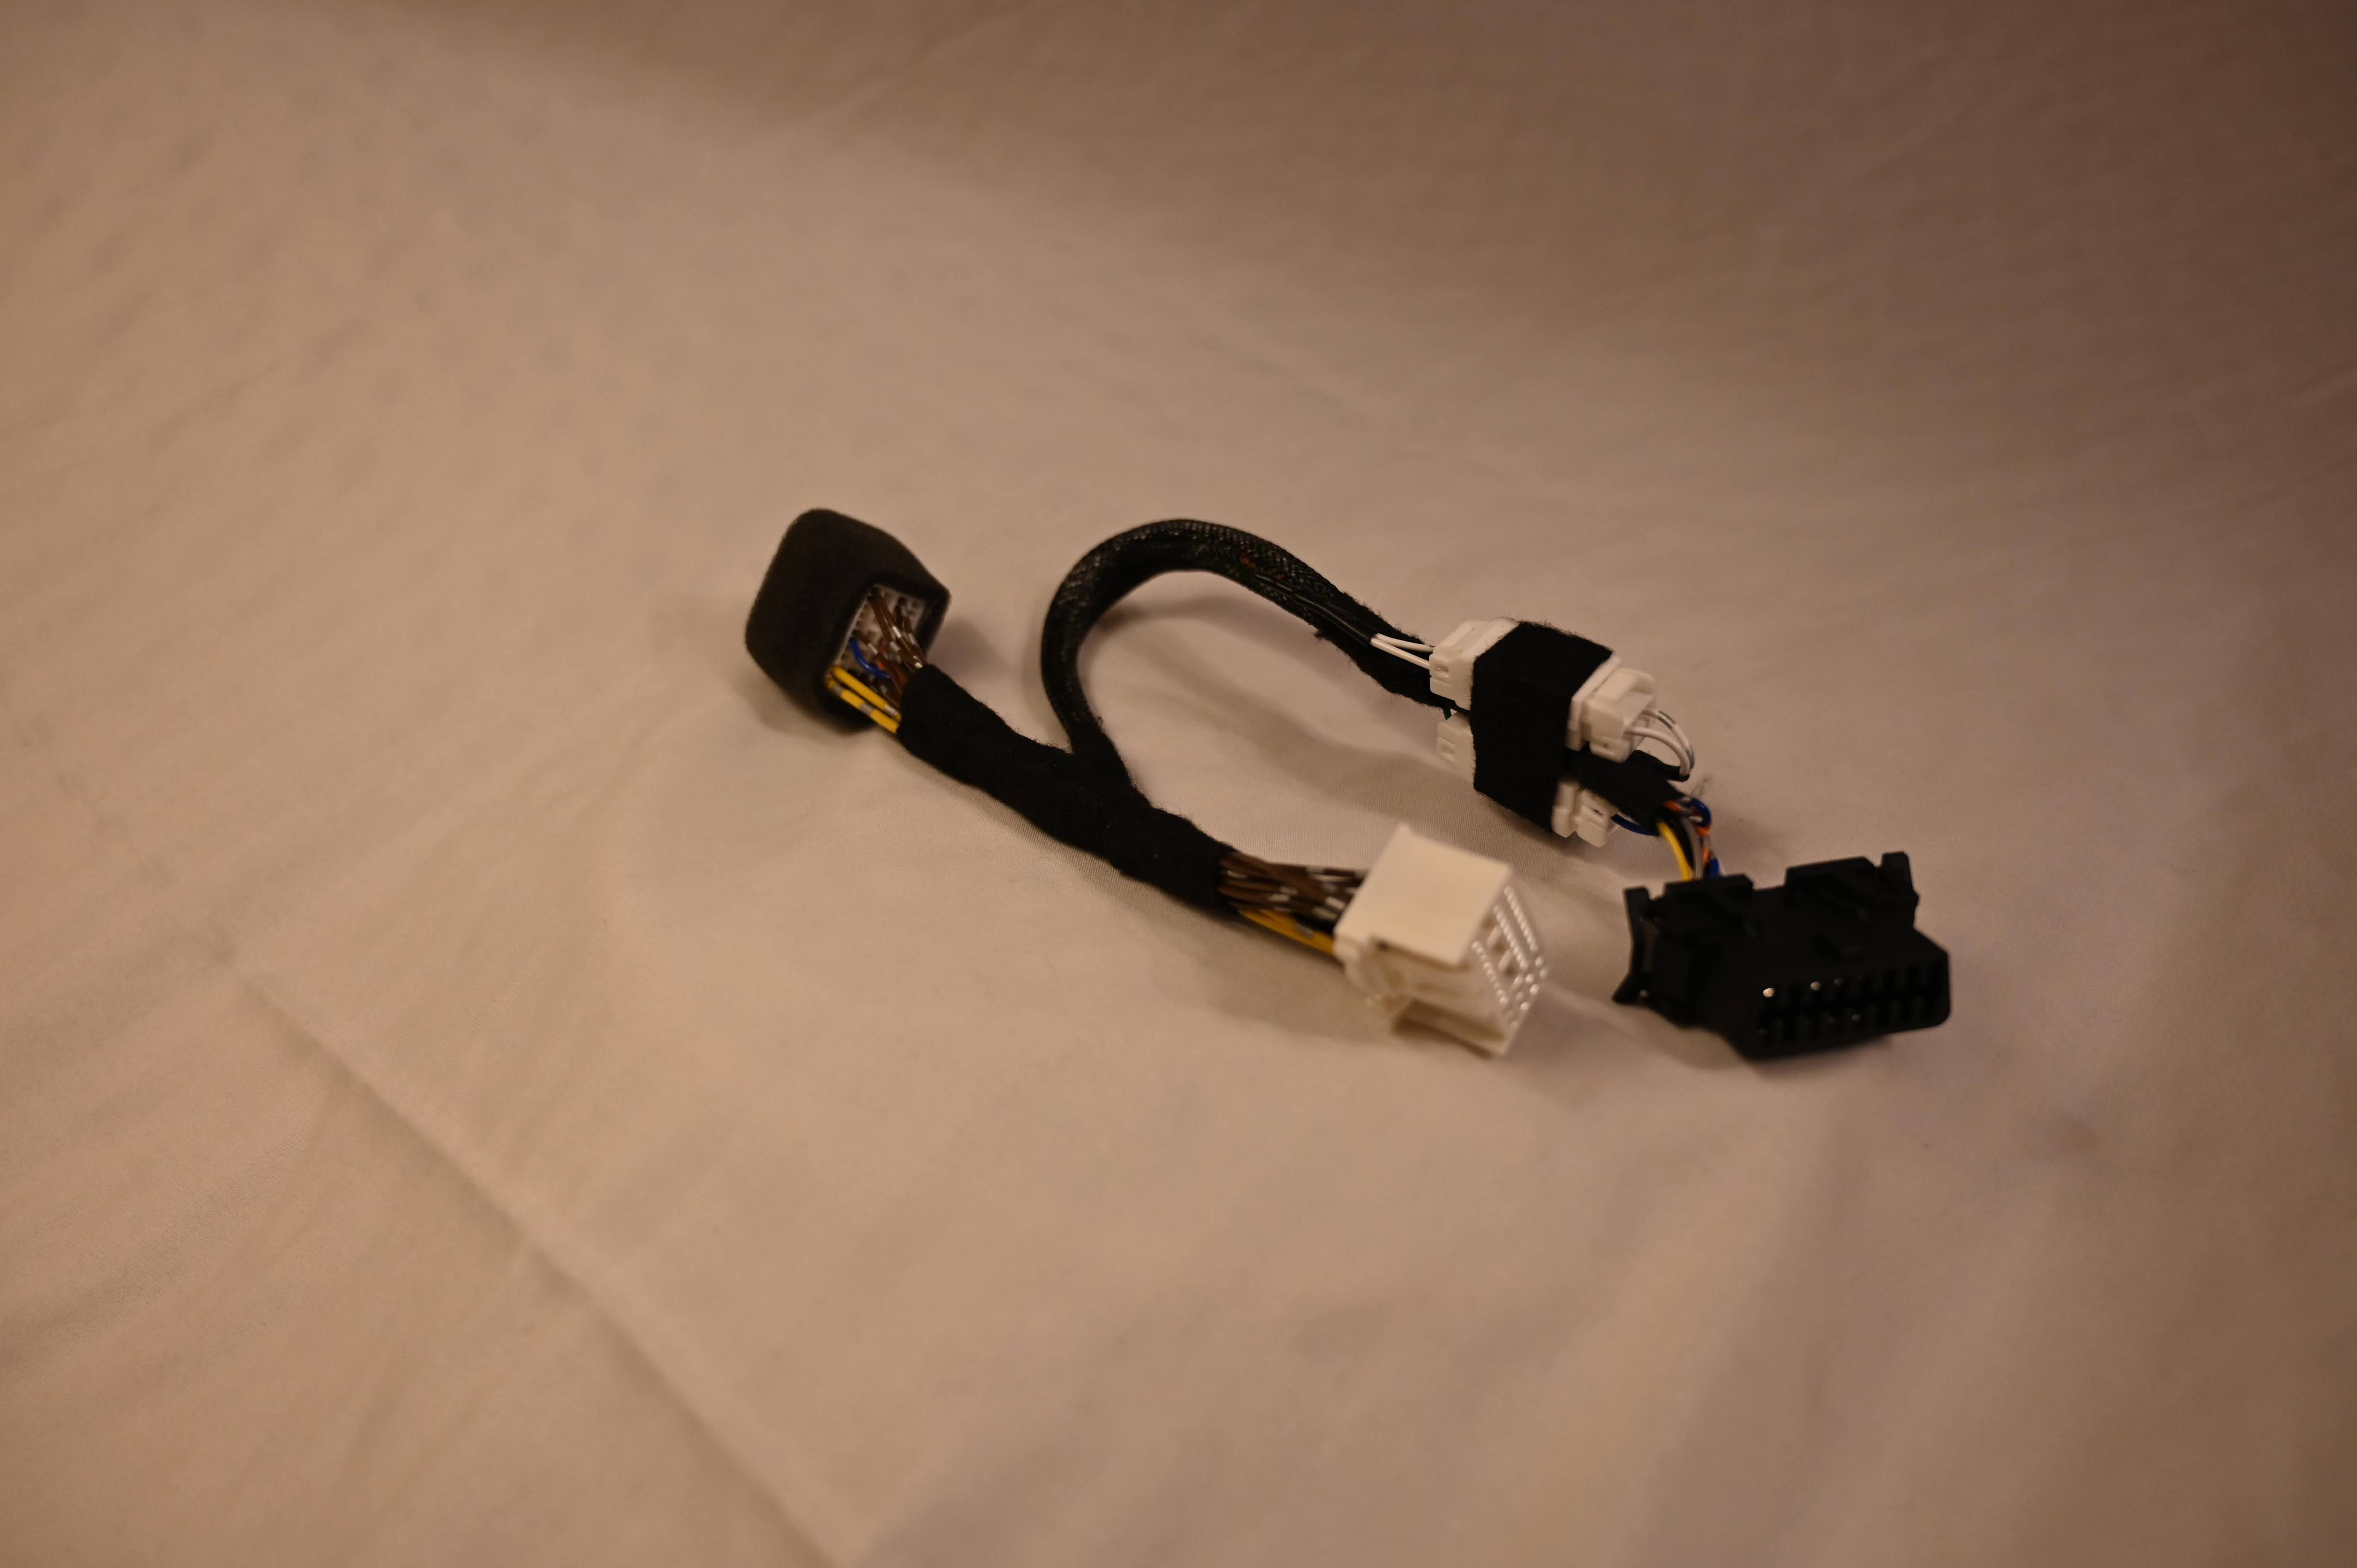
\includegraphics[height=1.95in]{../../../harnesses/head_unit_MITM/photos/whole_harness.jpg} } \\
  \subfloat[]{\label{subfig:overview:trim}
  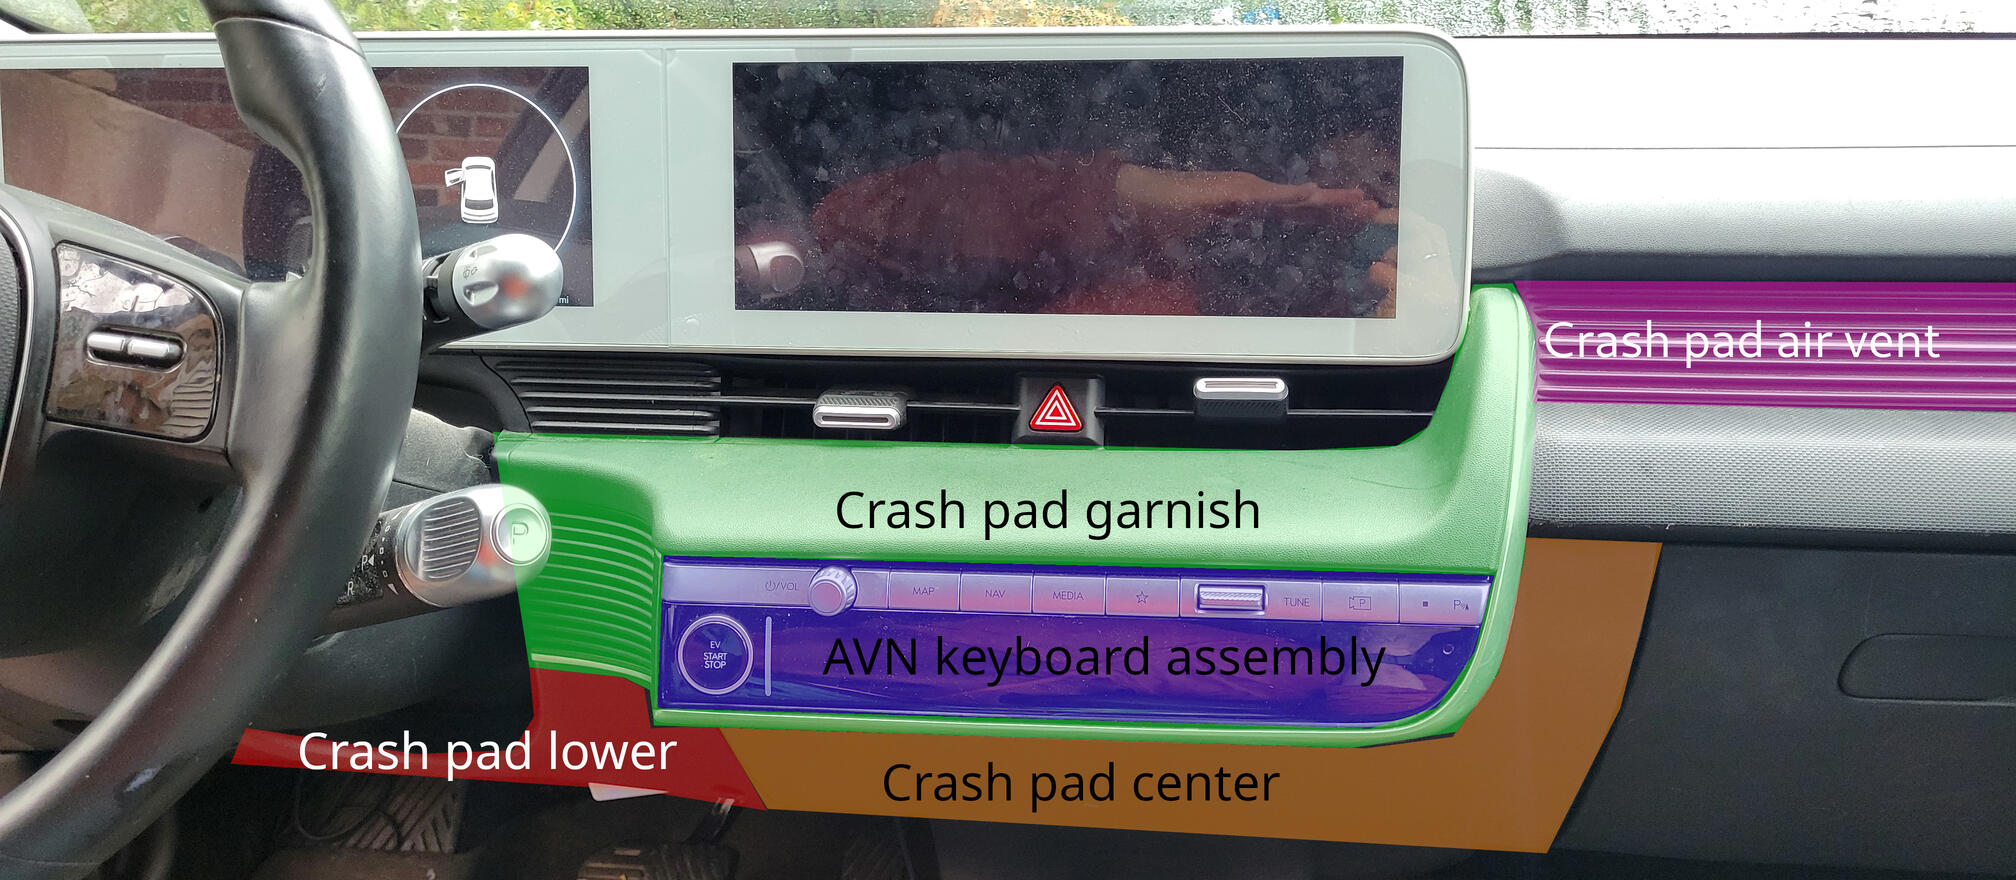
\includegraphics[width=6in]{photos/overview_labeled.jpg} }
   \caption{(a) Man-in-the-middle harness. (b) Overview of trim panels involved. \label{fig:overview}}
\end{figure}

\section{Introduction}
  The purpose of this guide is to illustrate step-by-step instructions for installing the head unit preconditioning kit, or just the head unit man-in-the-middle (MITM) harness, shown in Figure \ref{subfig:overview:harness}. In section \ref{sect:1}, we present two options for trim removal to access the head unit. In section \ref{sect:2}, we describe the process of plugging in the harness. In section \ref{sect:3}, we show attachment of the OBD port and how to plug in the microcontroller. 

\section{Step 1: Remove 12V Negative Terminal} \label{sect:0}
First, always disconnect the 12V battery before removing any electrical connectors! Removing a live electrical connector could cause a discharge and destroy a connector or ECU in your car.

Step-by-step instructions:
\begin{enumerate}
  \item Open hood (Figure \ref{subfig:12V:hood})
  \item Open frunk 
  \item Remove panel covering 12V (Figure \ref{subfig:12V:panel})
  \item Loosen nut on negative side with a 10mm socket (Figure \ref{subfig:12V:nut})
  \item Remove negative terminal (Figure \ref{subfig:12V:terminal})
\end{enumerate}

\begin{figure}[h]
  \subfloat[]{\label{subfig:12V:hood}
  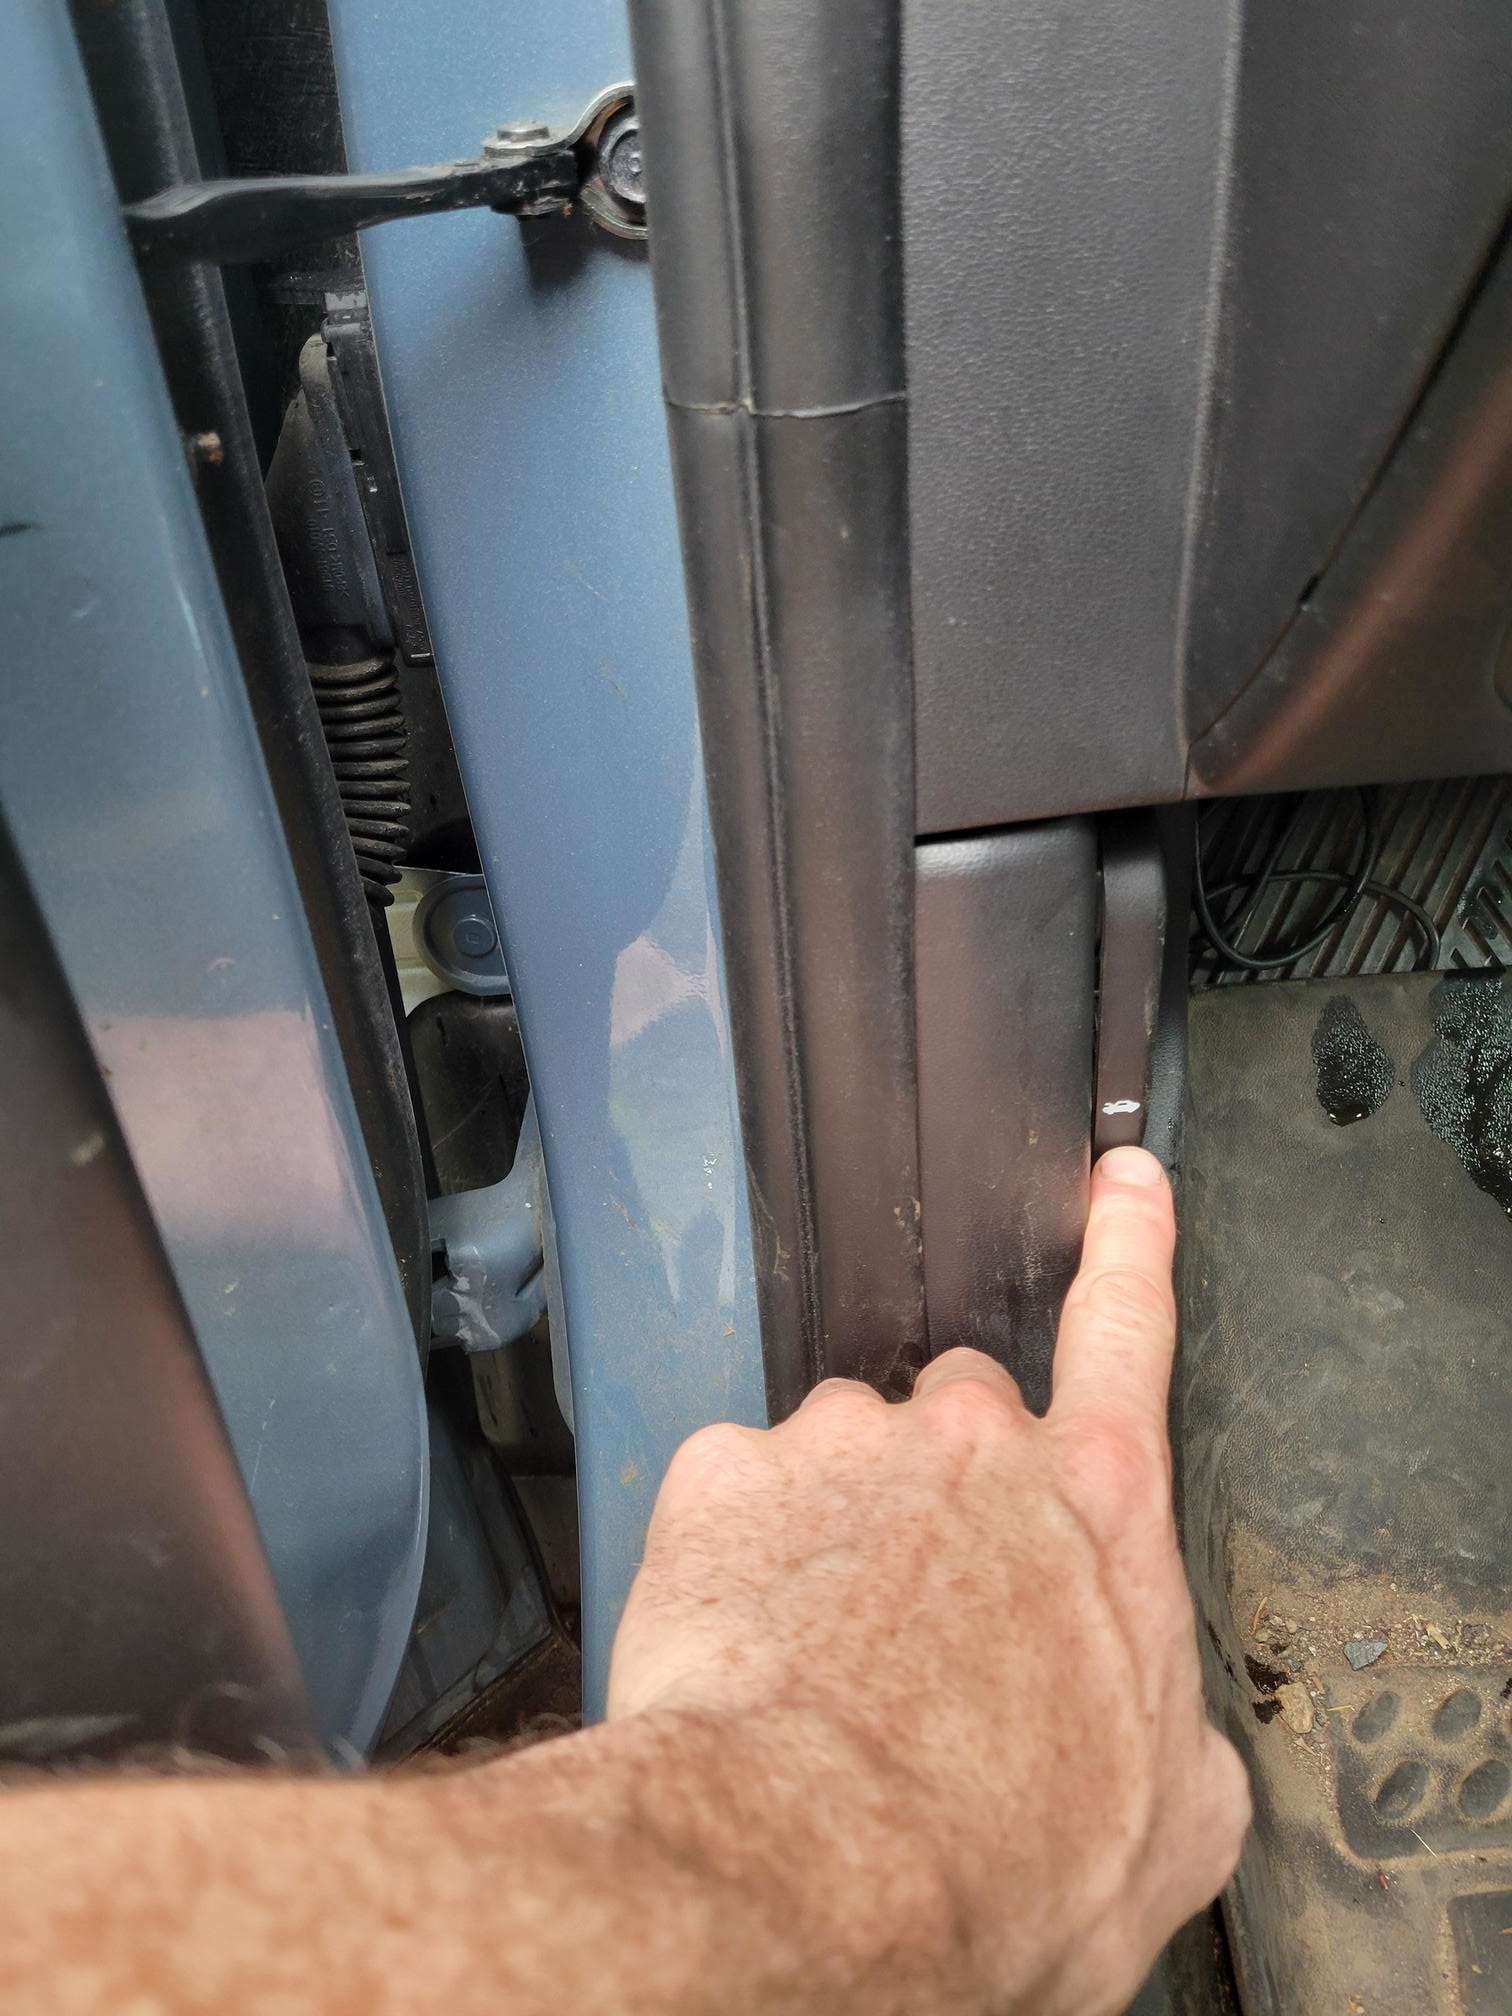
\includegraphics[height=1.5in]{photos/open_hood.jpg} } 
  \subfloat[]{\label{subfig:12V:panel}
  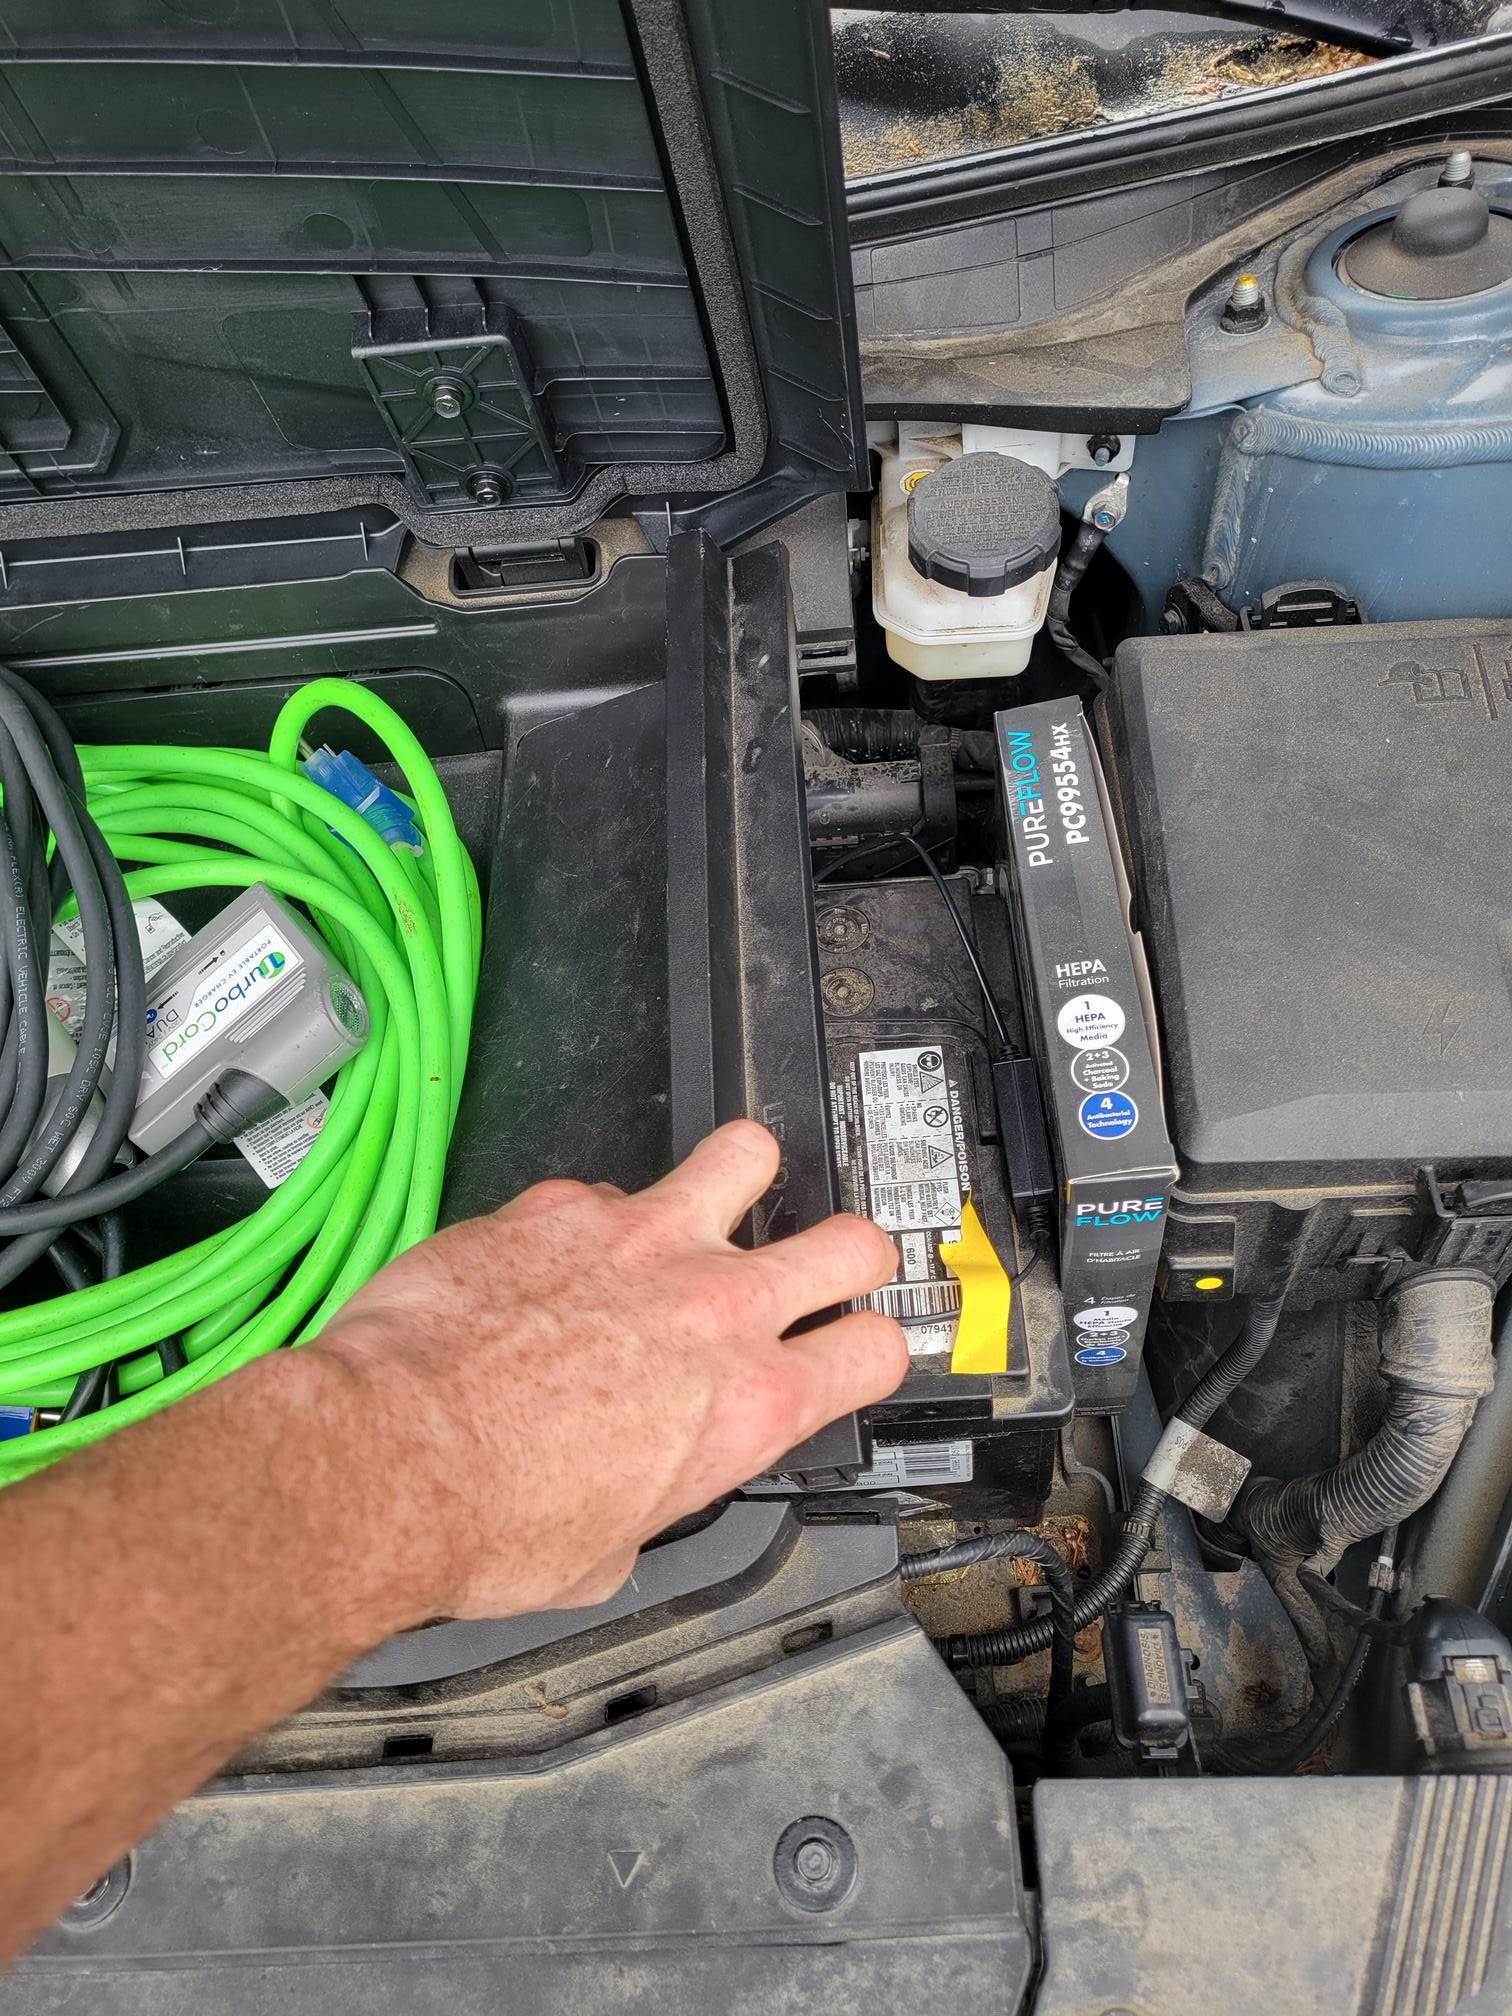
\includegraphics[height=1.5in]{photos/remove_panel.jpg} }  \\
  \subfloat[]{\label{subfig:12V:nut}
  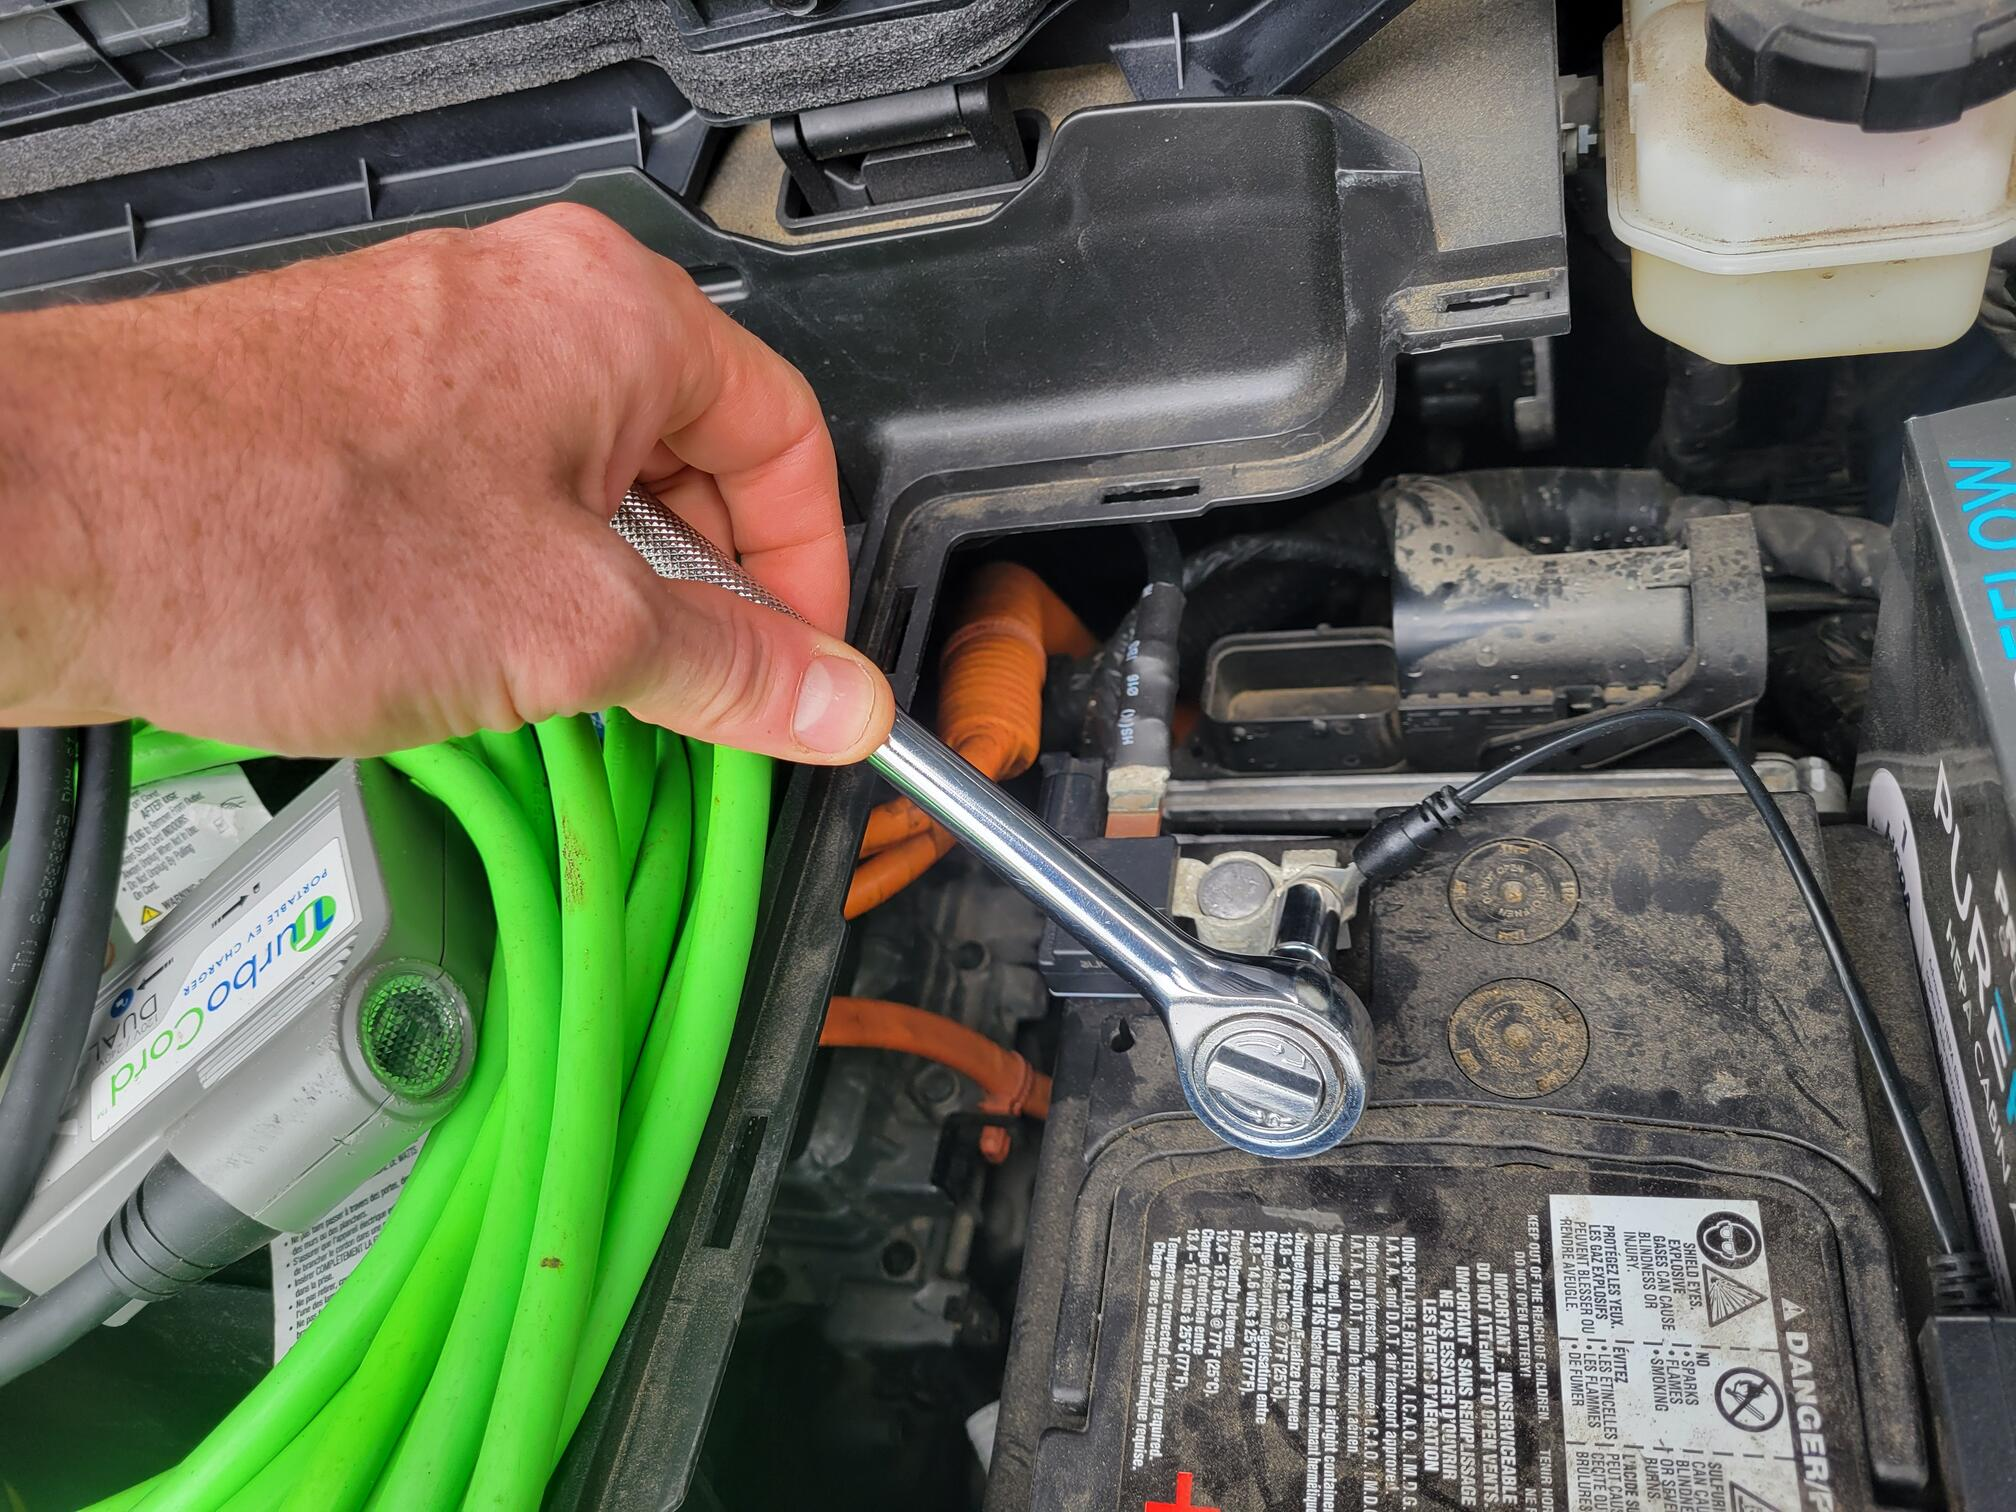
\includegraphics[height=1.5in]{photos/loosen_nut.jpg} } 
  \subfloat[]{\label{subfig:12V:terminal}
  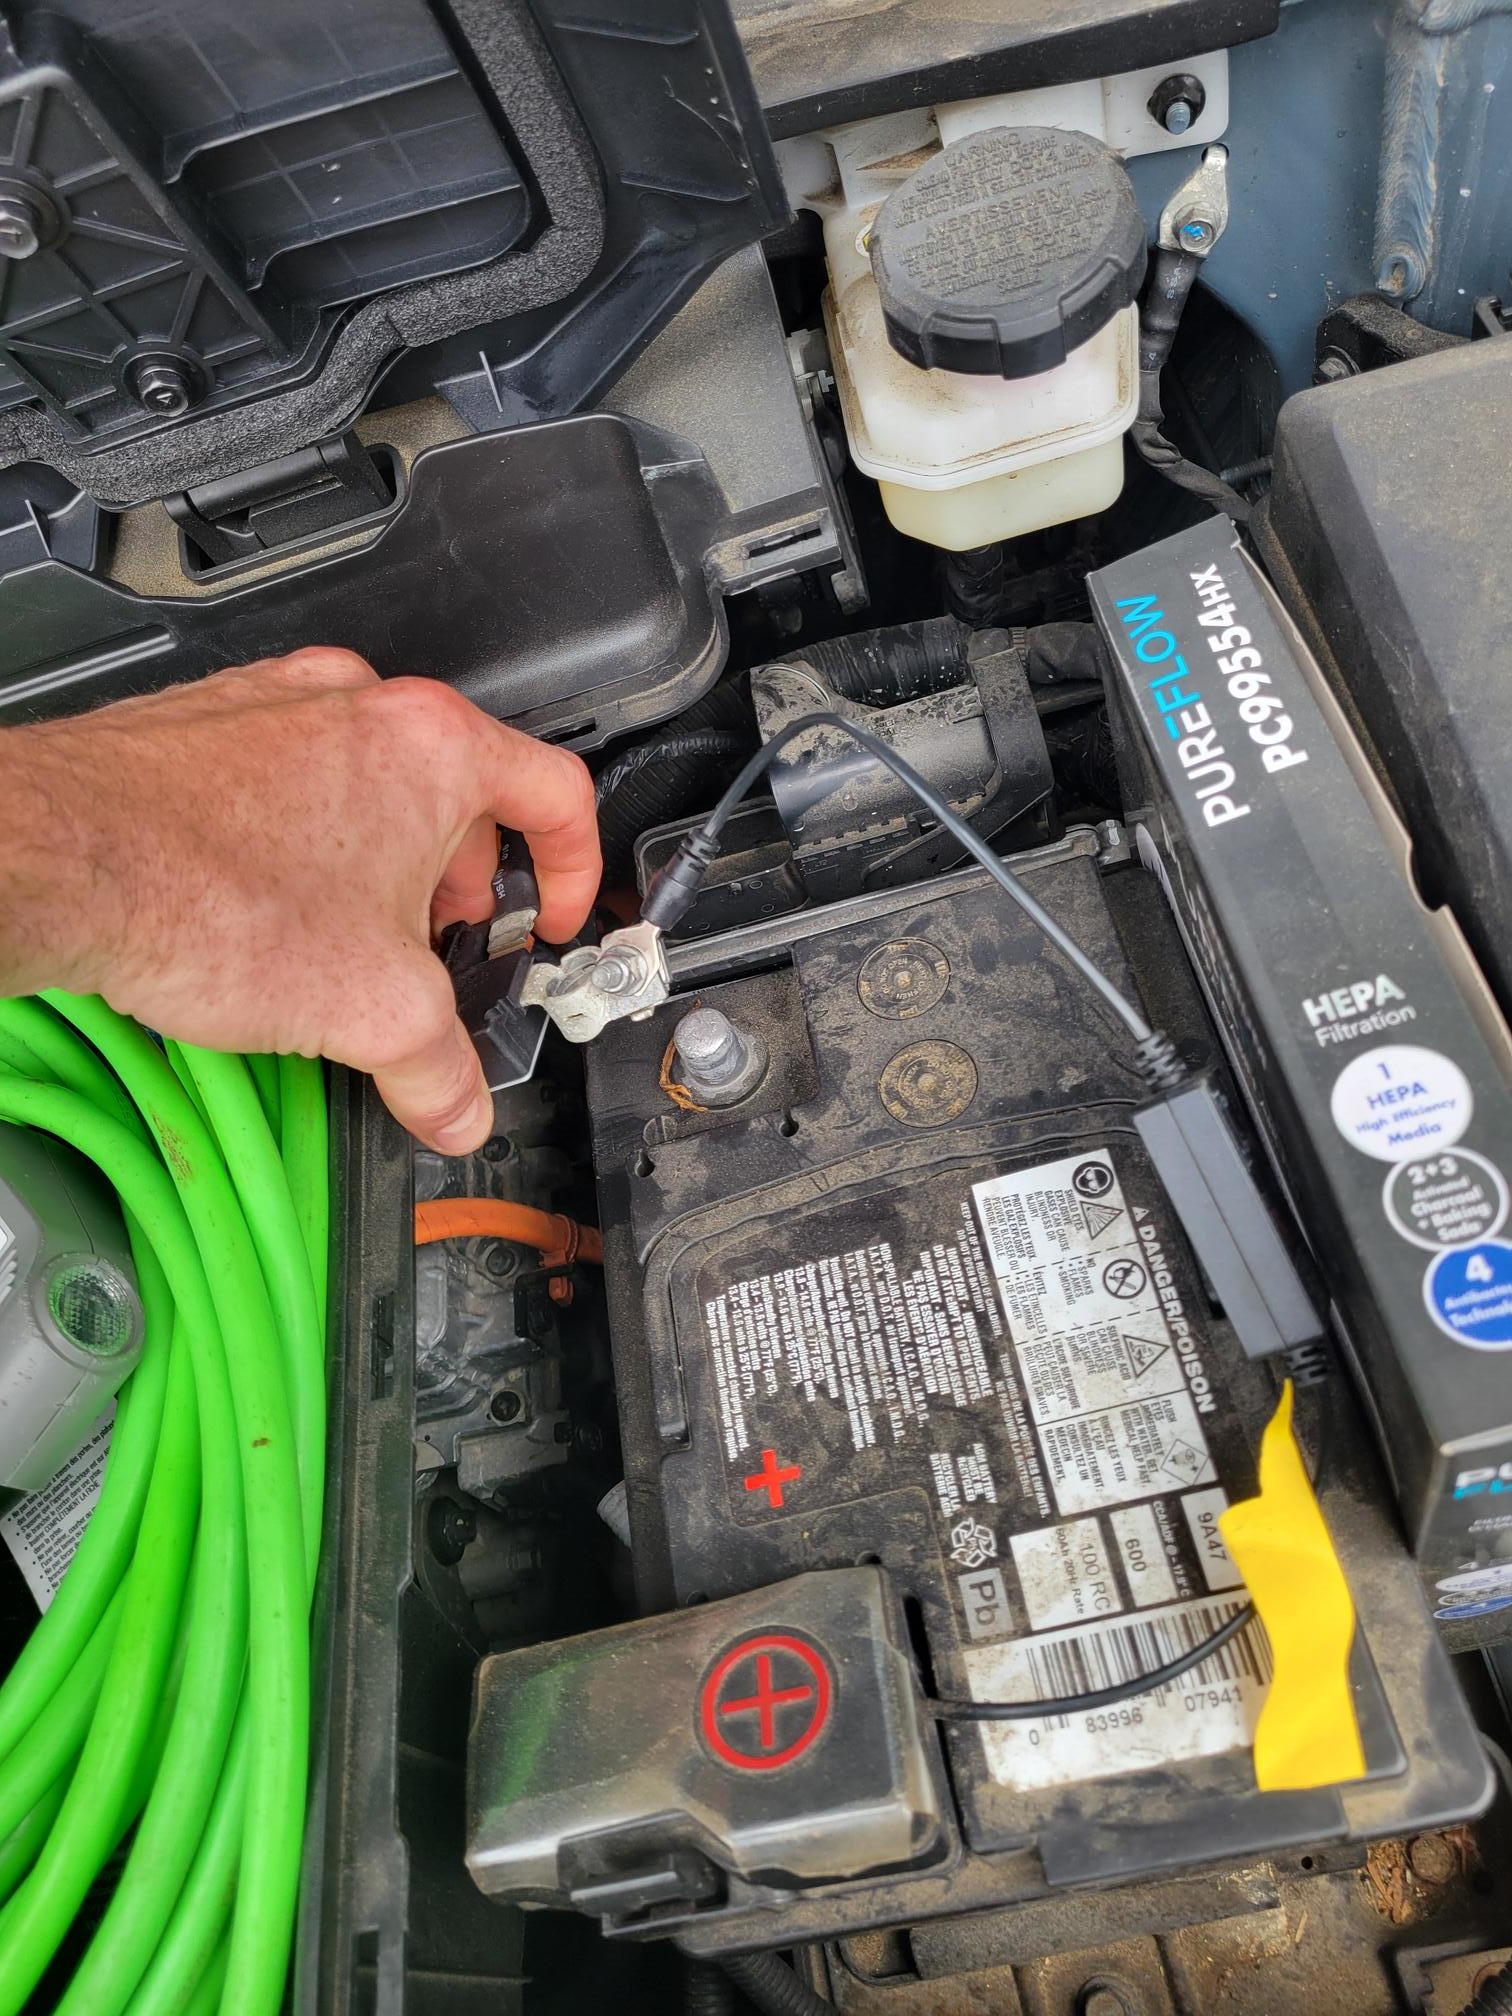
\includegraphics[height=1.5in]{photos/disconnect_terminal.jpg} } 
   \caption{(a) Open the hood. (b) Remove panel covering 12V. (c) Loosen nut on negative terminal. (d) Remove negative terminal. \label{fig:12V}}
\end{figure}

\section{Step 2: Trim} \label{sect:1}
The goal here is to get to the treasure chest: the head unit. The proper way involves removal 4 trim pieces and the AVN keyboard (climate button bar). It's also possible to take a shortcut. The shortcut is much faster but more awkward, with a higher risk of catching a hand on a sharp trim edge. Choose the method that works best for you.
\begin{figure}[h]
  \subfloat[]{\label{subfig:step1:X}
  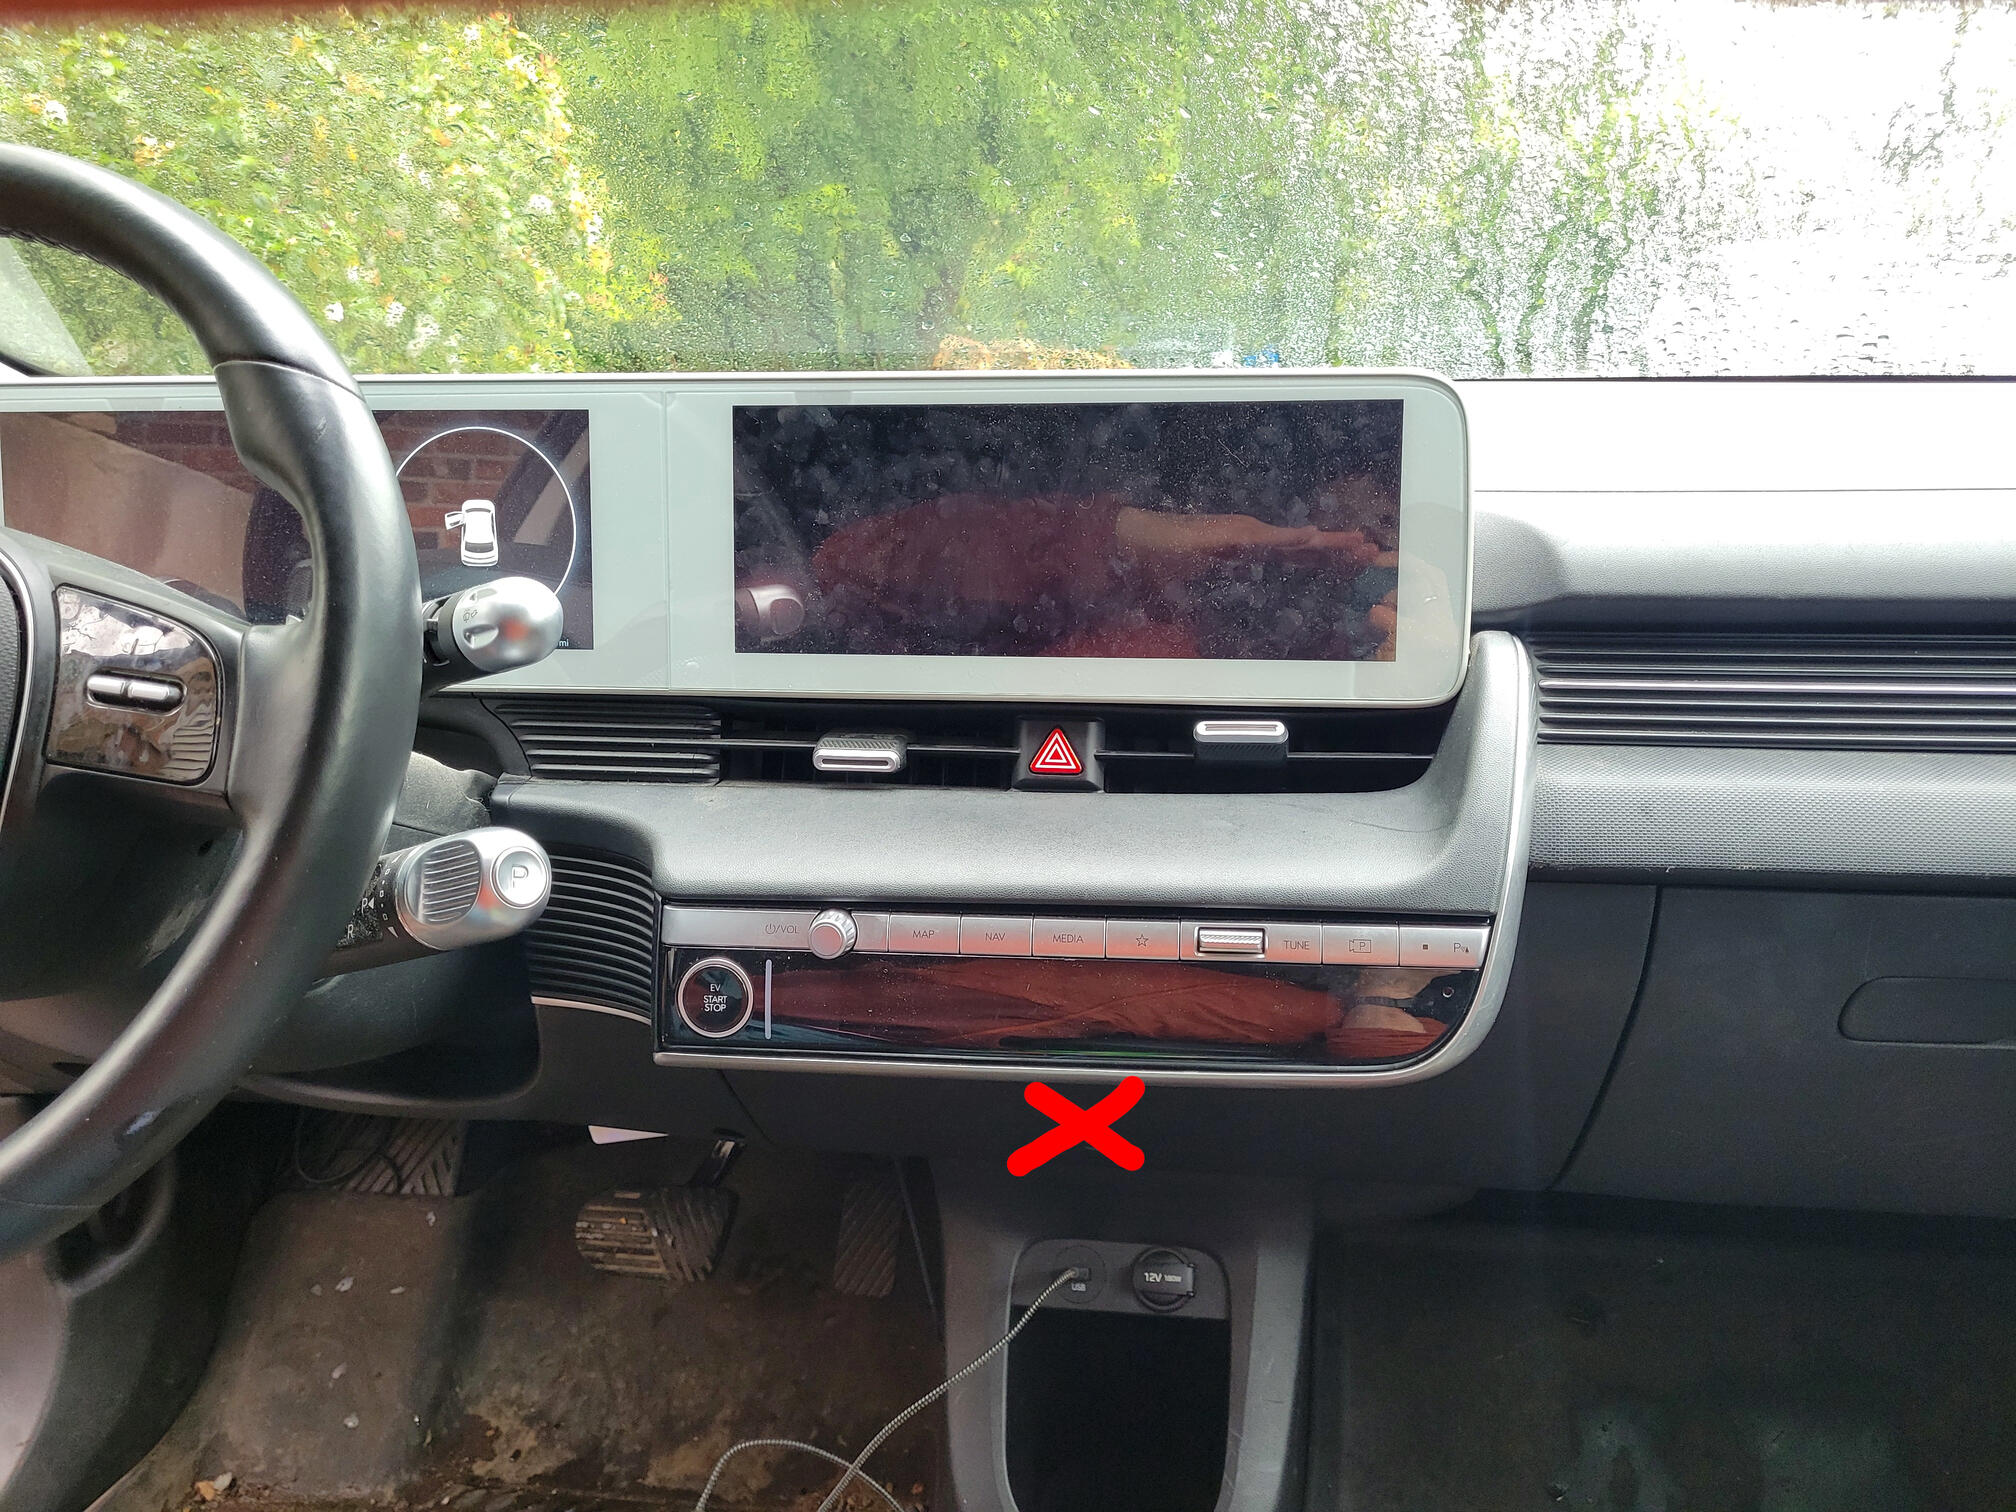
\includegraphics[height=2.95in]{photos/overview_X.jpg} } 
   \caption{X marks the head unit. \label{fig:step1}}
\end{figure}

\begin{figure}[h]
  \subfloat[]{\label{subfig:trim:lower}
  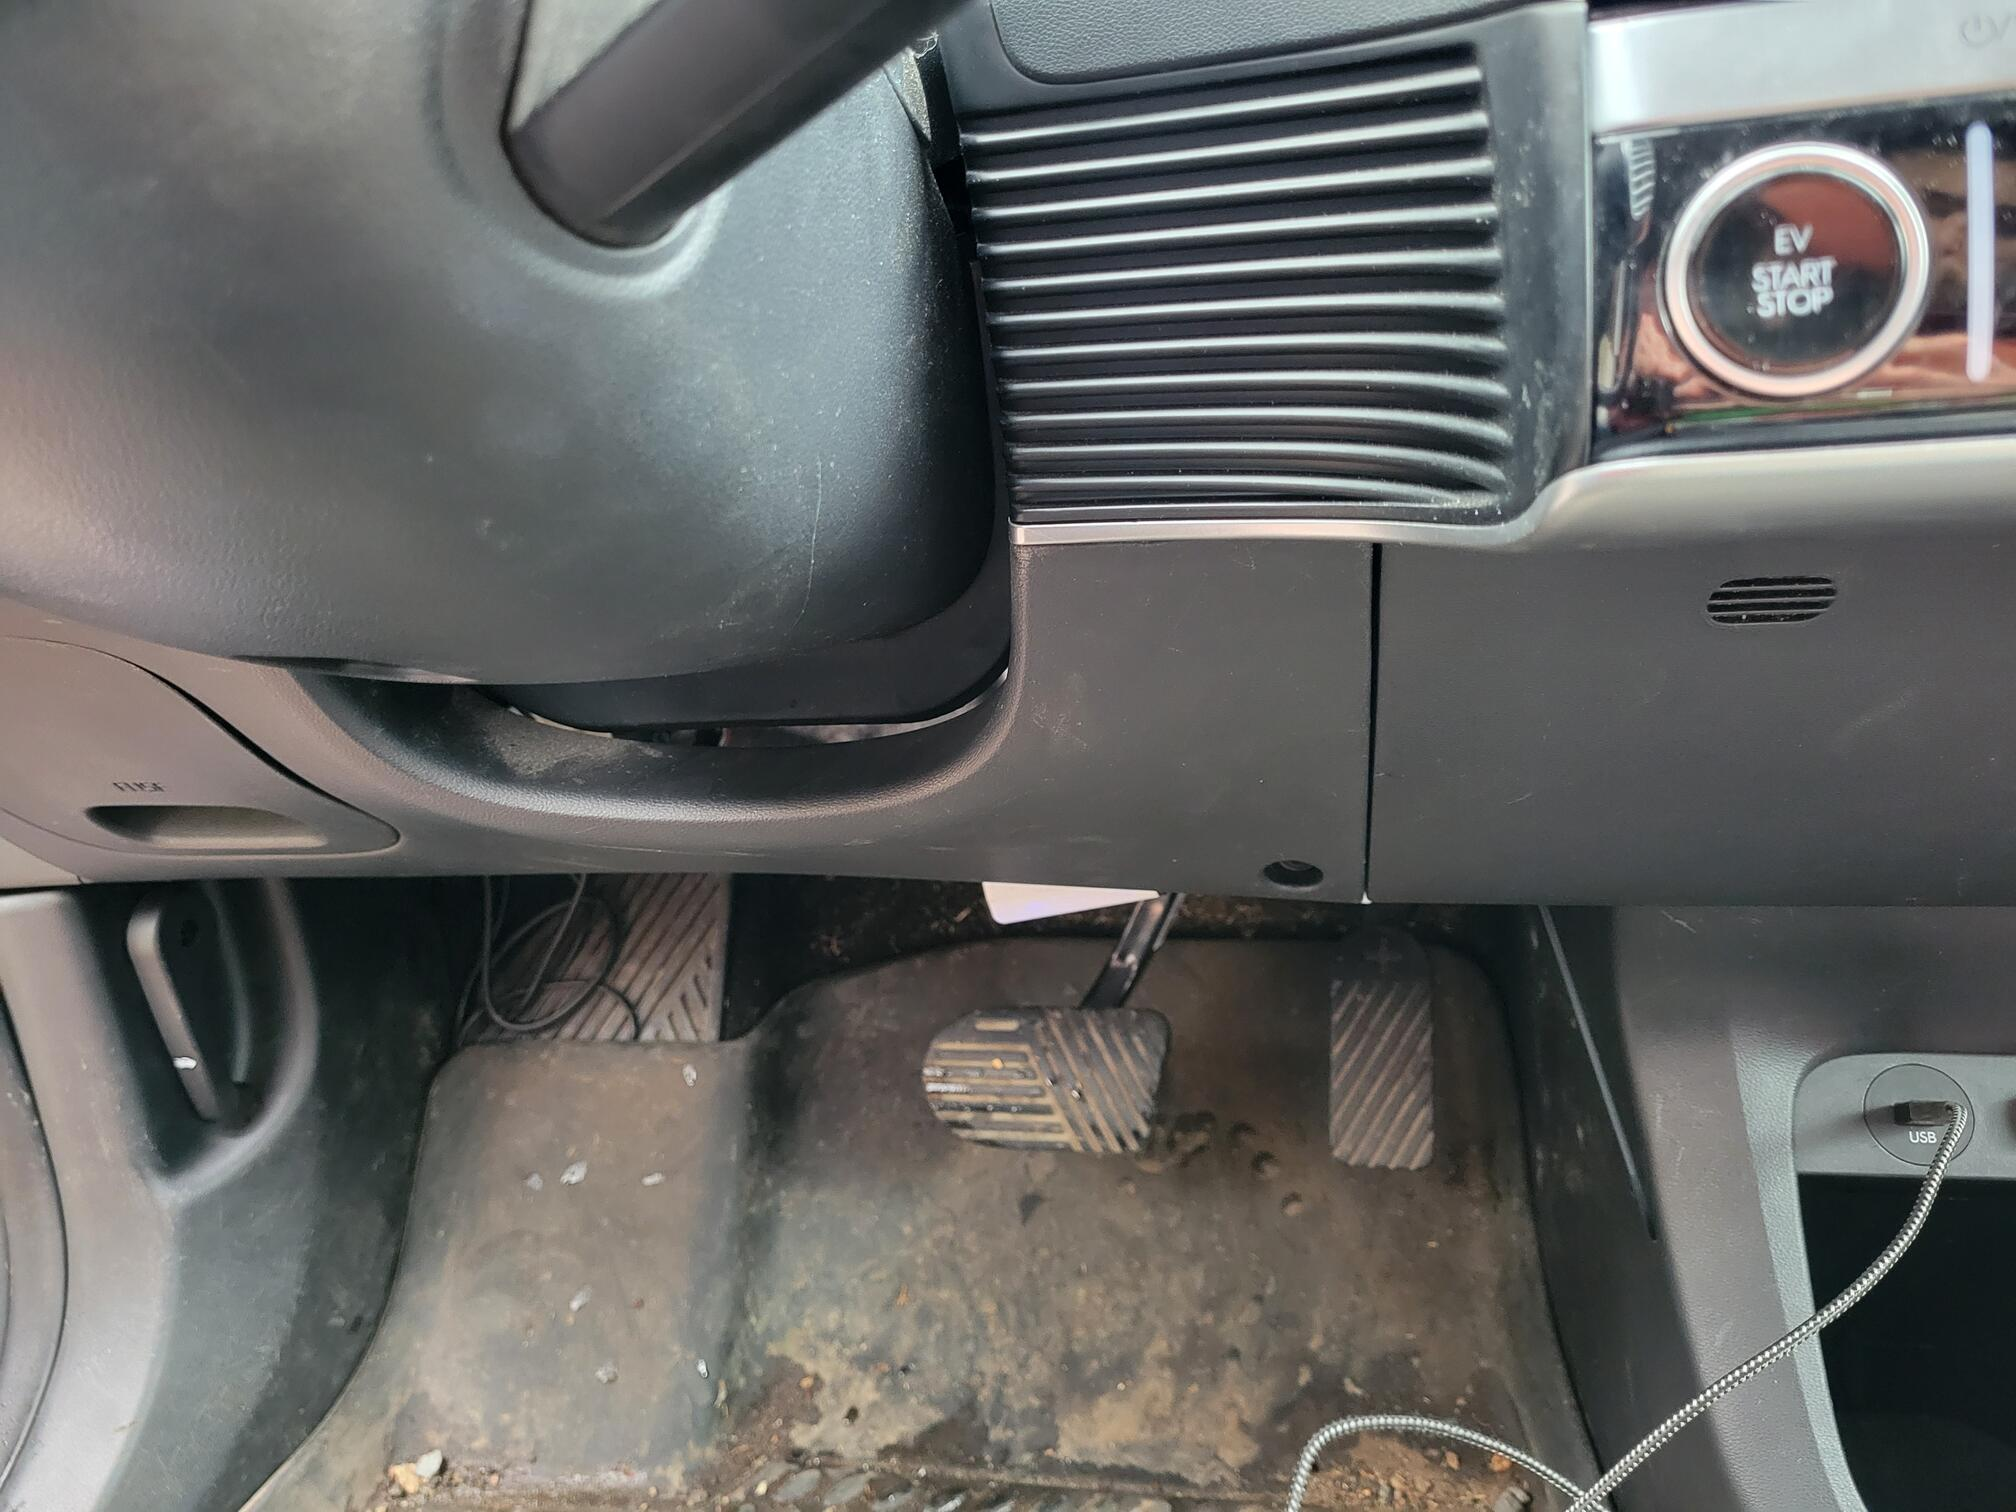
\includegraphics[height=1.5in]{photos/crash_pad_lower.jpg} } 
  \subfloat[]{\label{subfig:trim:airvent}
  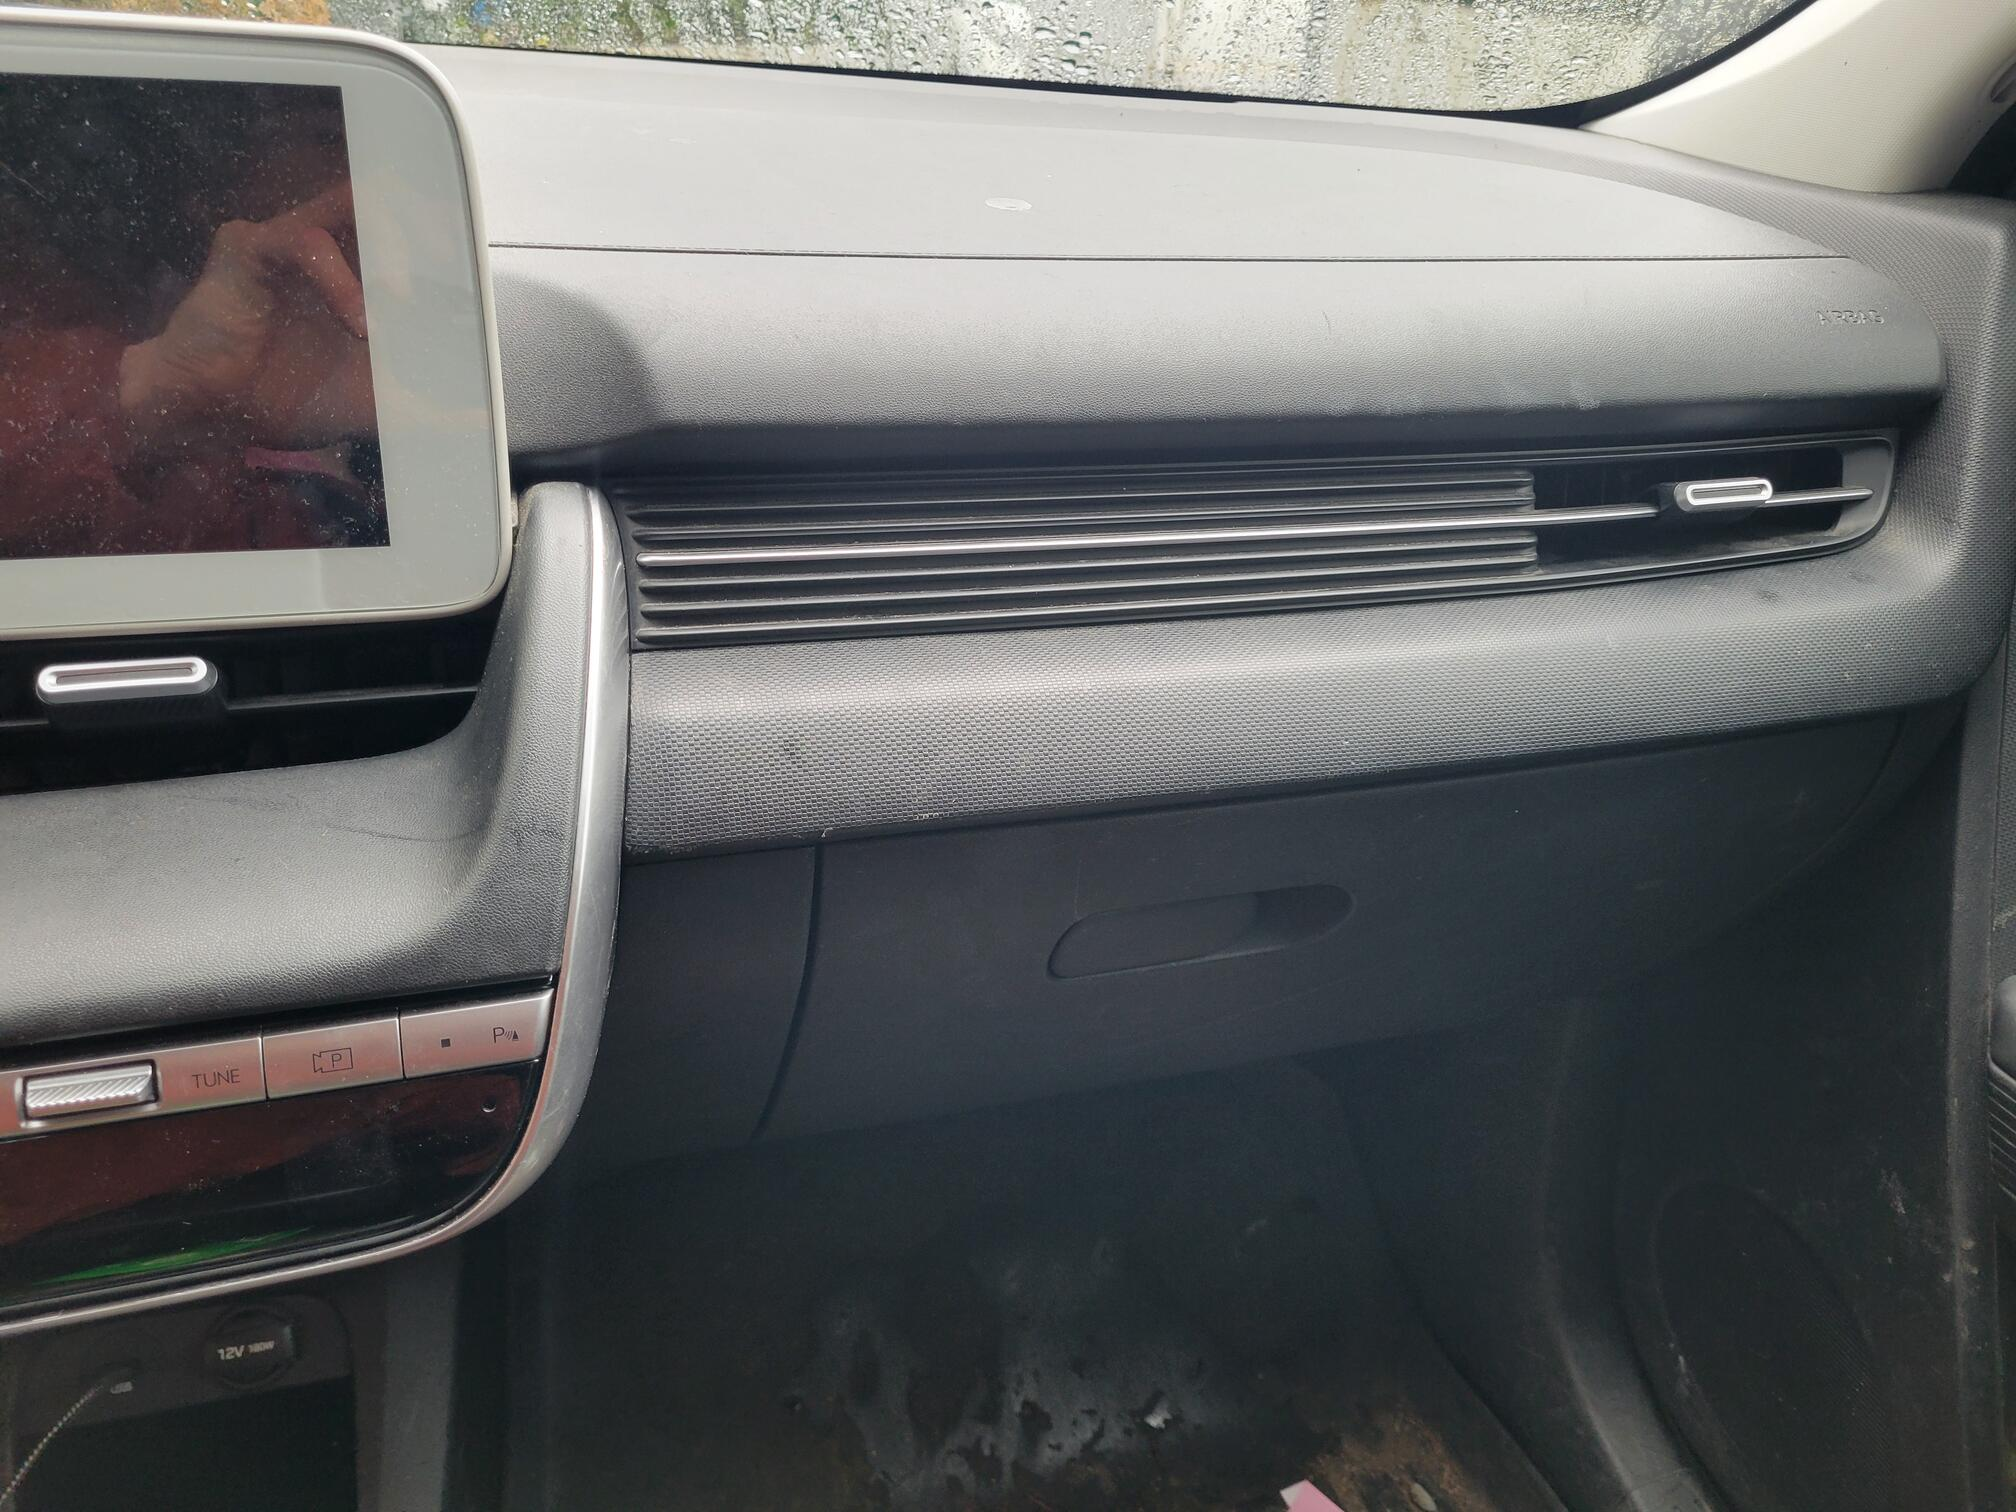
\includegraphics[height=1.5in]{photos/crash_pad_air_vent.jpg} } 
  \subfloat[]{\label{subfig:trim:center}
  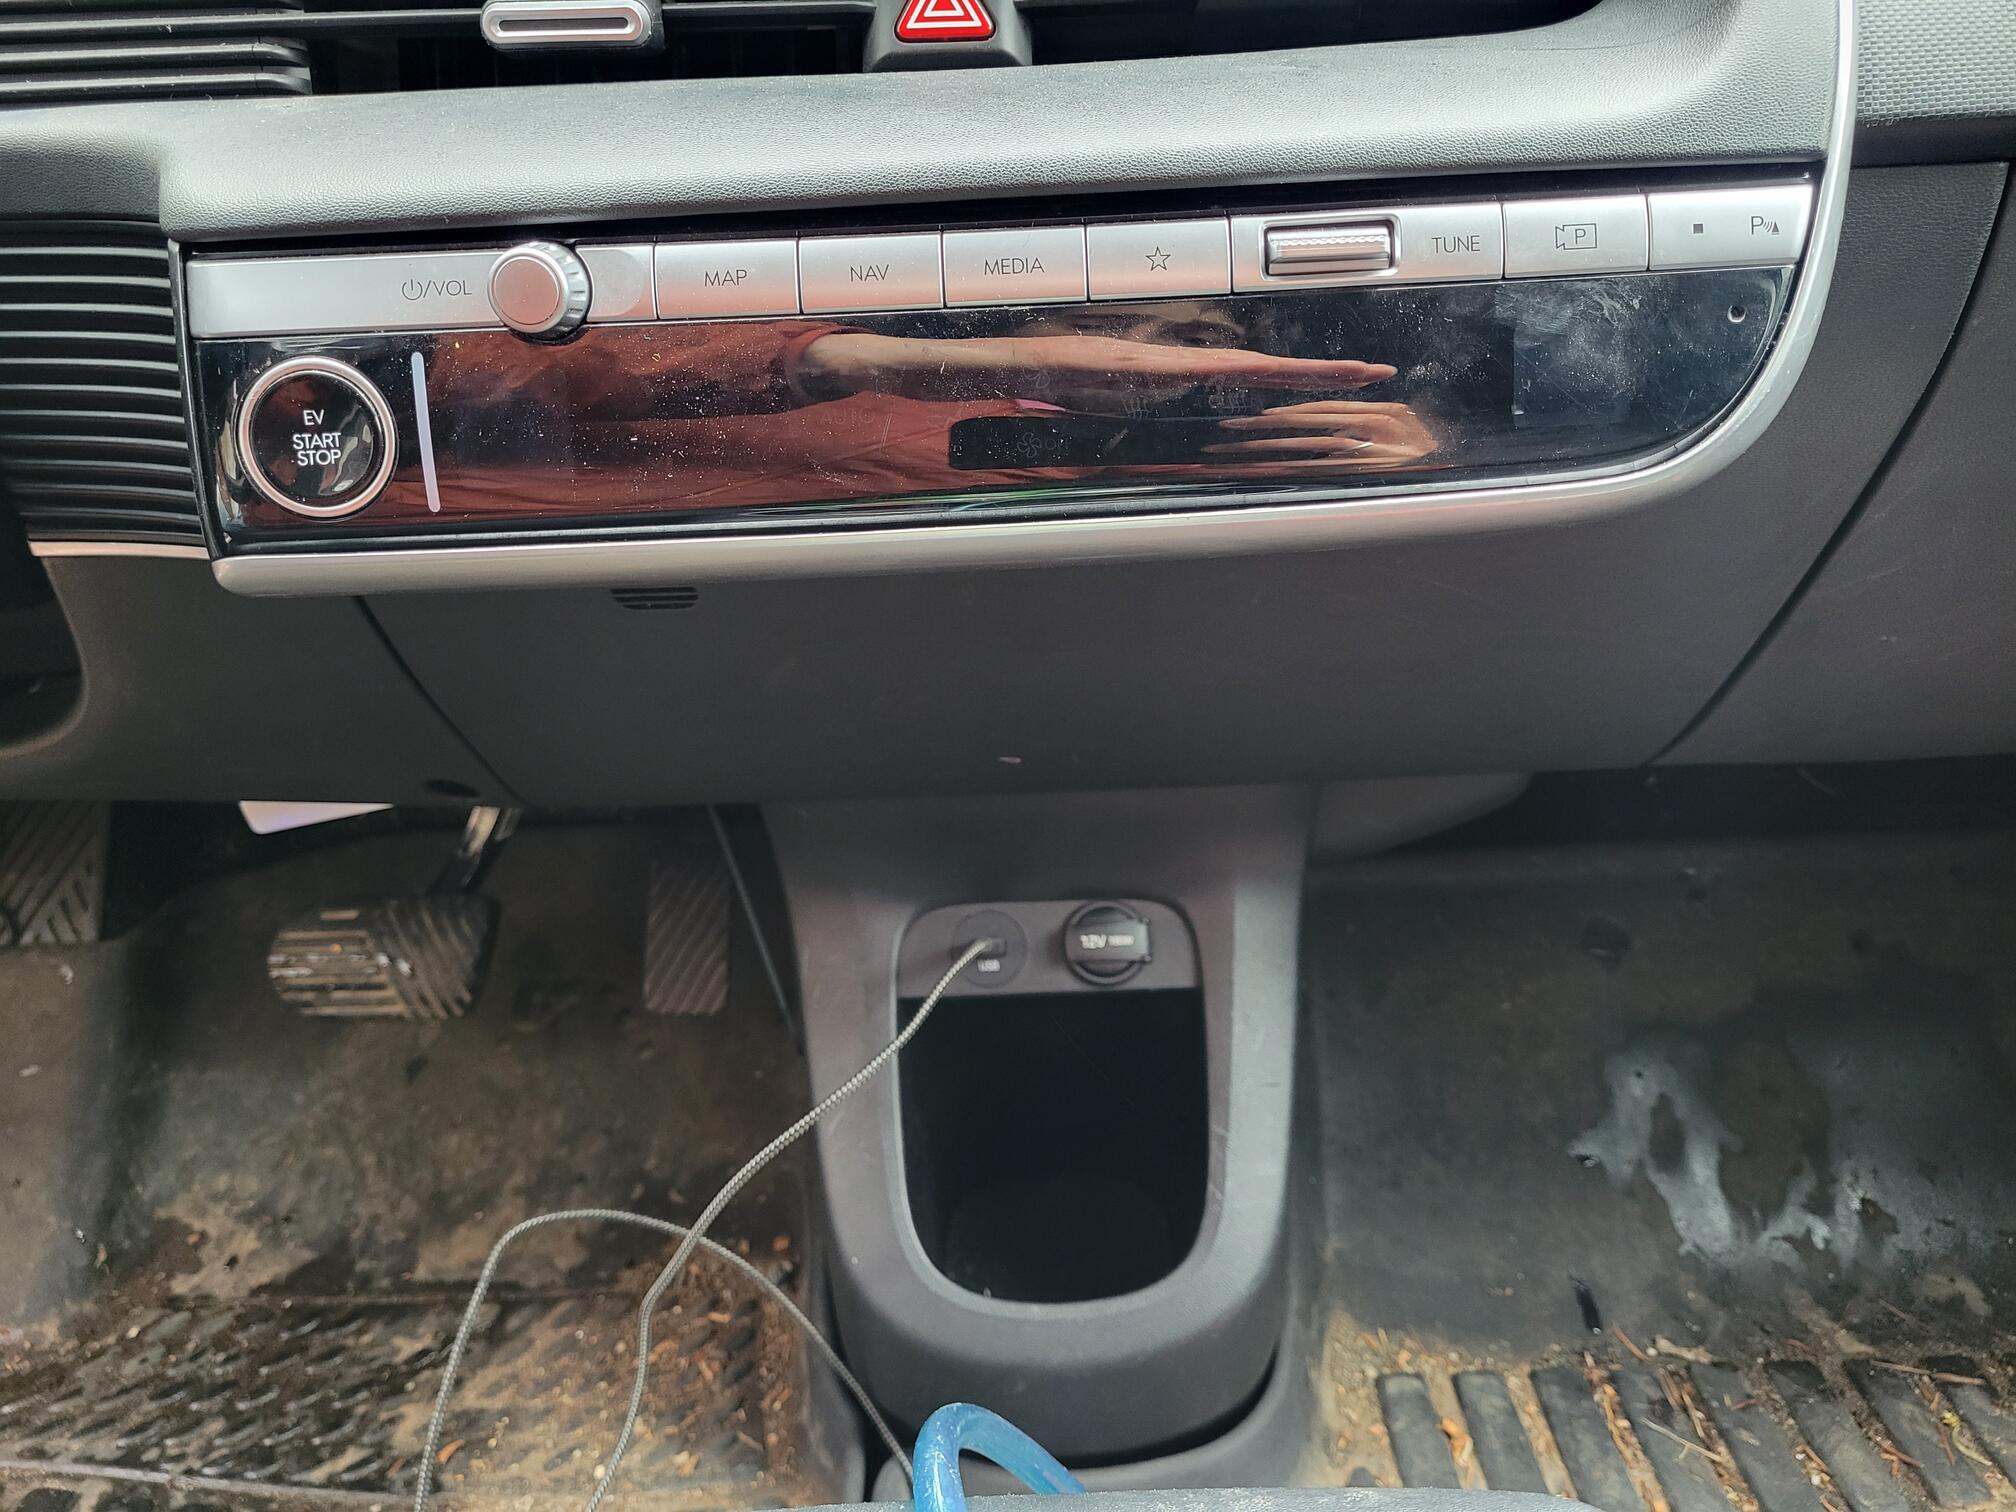
\includegraphics[height=1.5in]{photos/crash_pad_center_and_keyboard.jpg} } 
   \caption{(a) Crash pad lower. (b) Crash pad air vent. (c) Crash pad garnish, AVN keyboard, and crash pad center. \label{fig:trim}}
\end{figure}

\subsection{Option A: long and careful}
Trim panel order of operations: 
\begin{enumerate}
  \item Crash pad lower (Figure \ref{subfig:trim:lower}) \label{step:cpl}
  \item Crash pad air vent (Figure \ref{subfig:trim:airvent}) \label{step:cpav}
  \item Crash pad garnish (Figure \ref{subfig:trim:center})
  \item AVN keyboard (Figure \ref{subfig:trim:center})
  \item Crash pad center (Figure \ref{subfig:trim:center})
\end{enumerate}

Steps \ref{step:cpl} and \ref{step:cpav} can be done in either order; both must be done to free the crash pad garnish.

Step-by-step instructions:
\begin{enumerate}
  \item Remove screw in crash pad lower (Figure \ref{subfig:trimsteps:lowerscrew})
  \item Pull off right half of crash pad lower using trim removal tools
  \item While here, remove screw behind crash pad lower; this screw tends to remain captive, so you have to pull to confirm it's out (Figure \ref{subfig:trimsteps:cpc_llscrew})
  \item Remove crash pad air vent
  \item Remove screw that was hidden behind crash pad air vent (Figure \ref{subfig:trimsteps:cpg_r_screw})
  \item Remove crash pad garnish
  \item Detach AVN keyboard 
    \begin{enumerate}
      \item Remove left screw (Figure \ref{subfig:trimsteps:keyboard_l_screw})
      \item Remove right screw (Figure \ref{subfig:trimsteps:keyboard_ur_screw})
      \item Remove lower left screw (Figure \ref{subfig:trimsteps:keyboard_ll_screw})
      \item Remove lower right screw (Figure \ref{subfig:trimsteps:keyboard_lr_screw})
      \item (optional, check for no 12V power) Remove all electrical connectors from rear of AVN keyboard
      \item Disconnect trim clips by pulling outwards on the keyboard (Figure \ref{subfig:trimsteps:remove_keyboard})
      \item If electrical connectors are still connected, avoid putting too much tension on them
    \end{enumerate}
  \item Remove crash pad center upper right screw that was blocked by AVN keyboard (Figure \ref{subfig:trimsteps:cpc_urscrew})
  \item (optional) Re-insert AVN keyboard for safekeeping if electrical connectors are still attached
  \item Remove crash pad center upper left screw (Figure \ref{subfig:trimsteps:cpc_ulscrew})
  \item Remove crash pad center trim panel using trim removal tools
  \item (check for no 12V power first) Disconnect electrical connector from back of panel and move it away from work area
\end{enumerate}

\begin{figure}[h]
  \subfloat[]{\label{subfig:trimsteps:lowerscrew}
  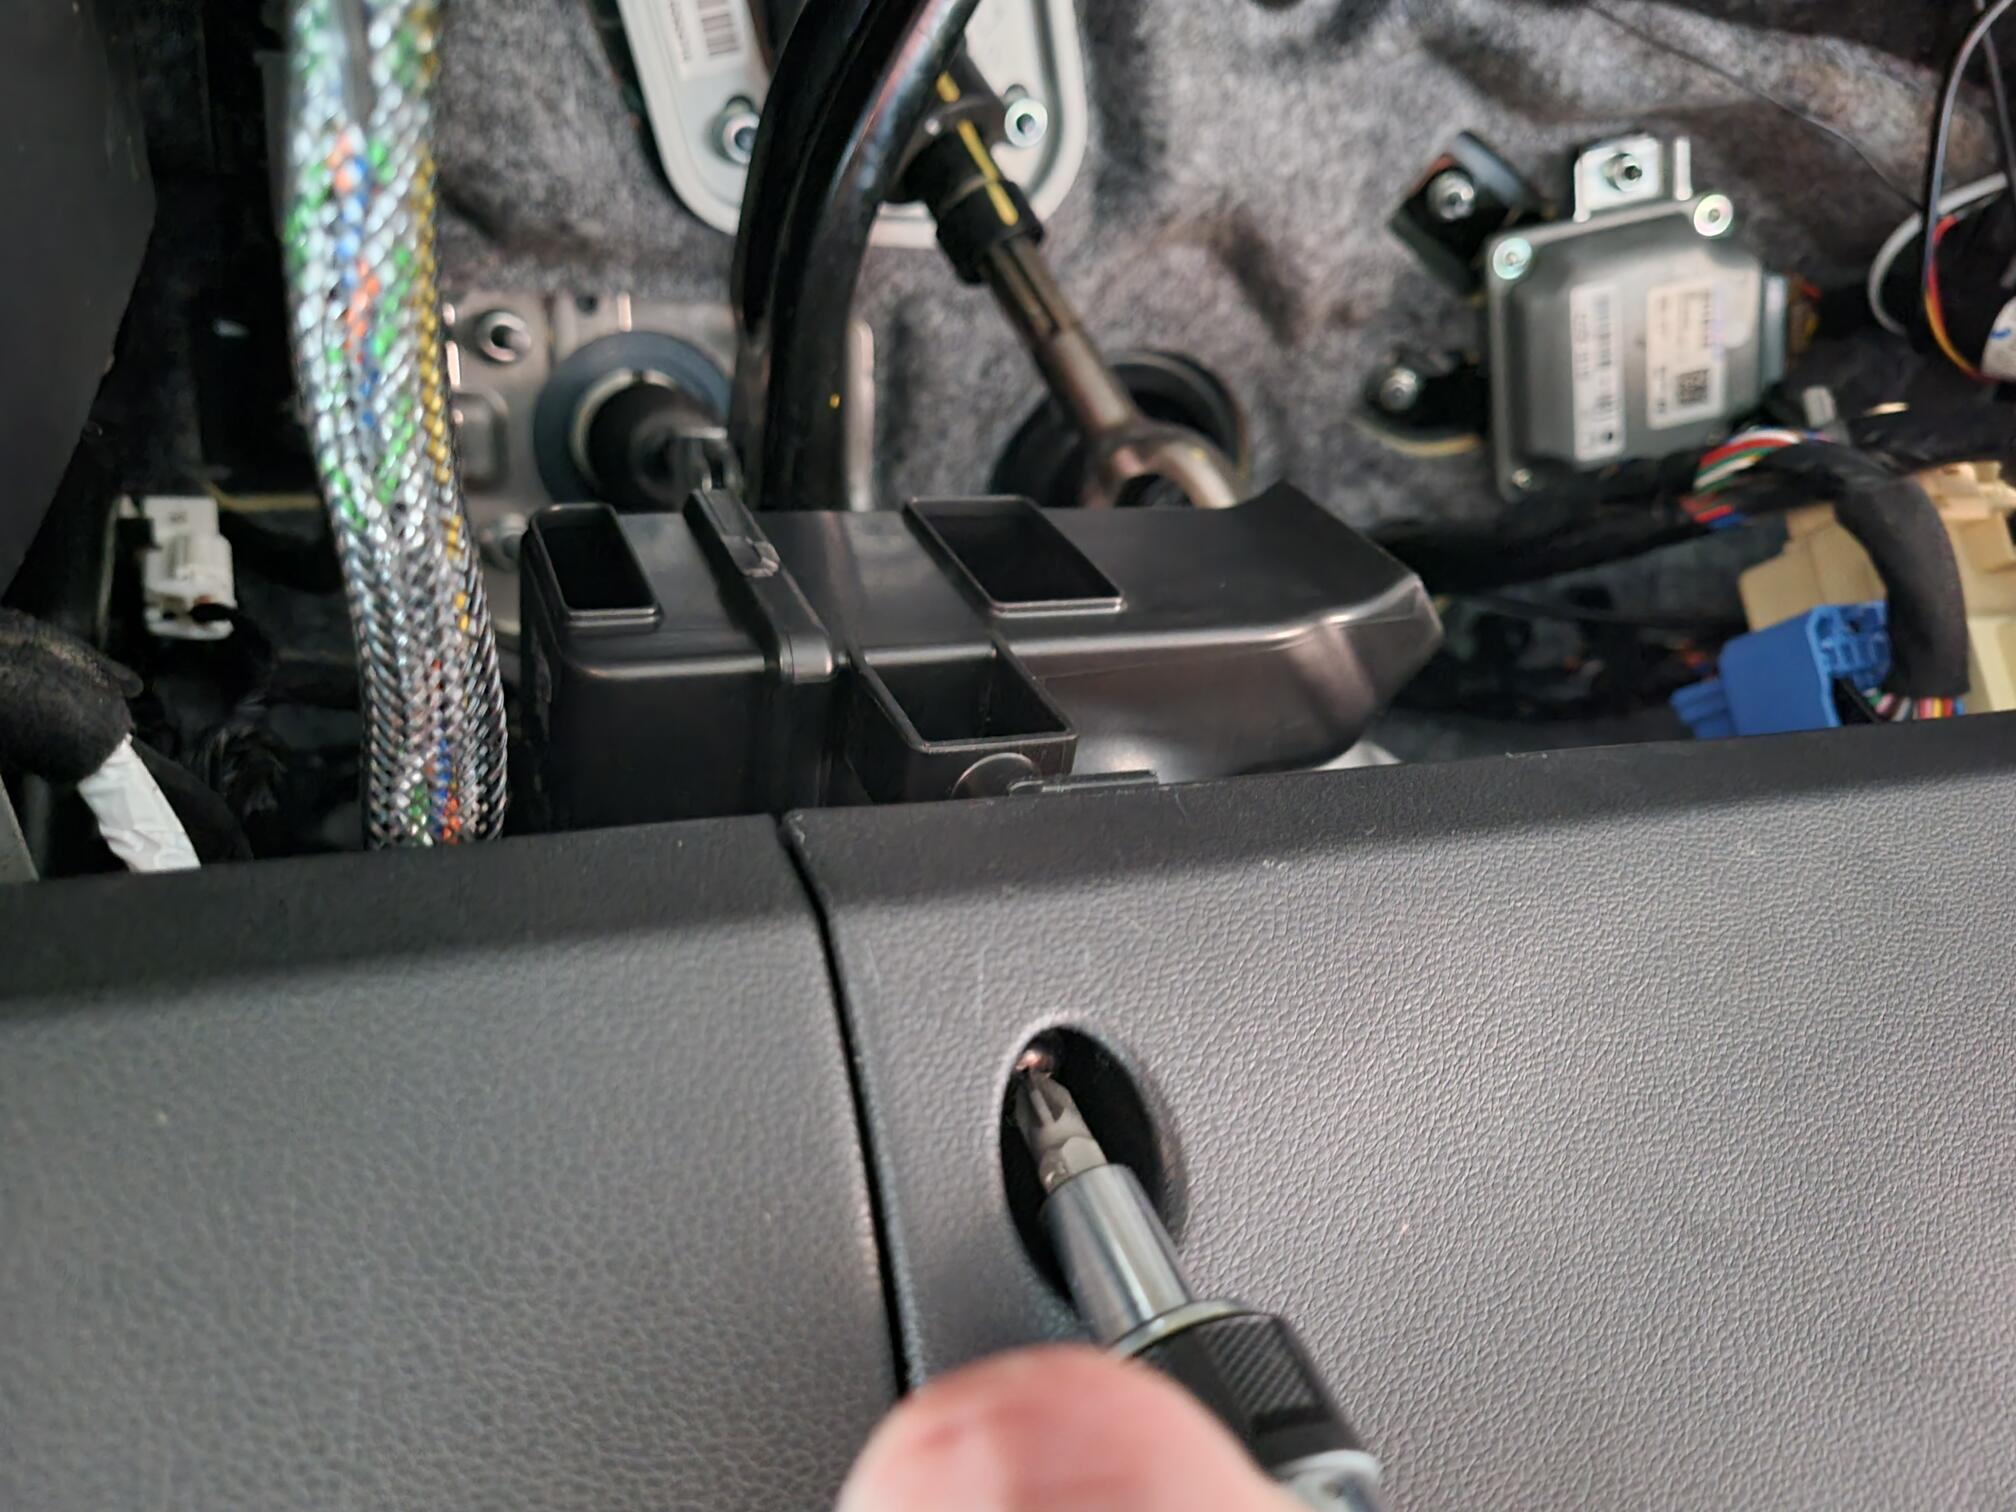
\includegraphics[height=1.5in,angle=180]{photos/crash_pad_lower_screw.jpg} } 
  \subfloat[]{\label{subfig:trimsteps:cpc_llscrew}
  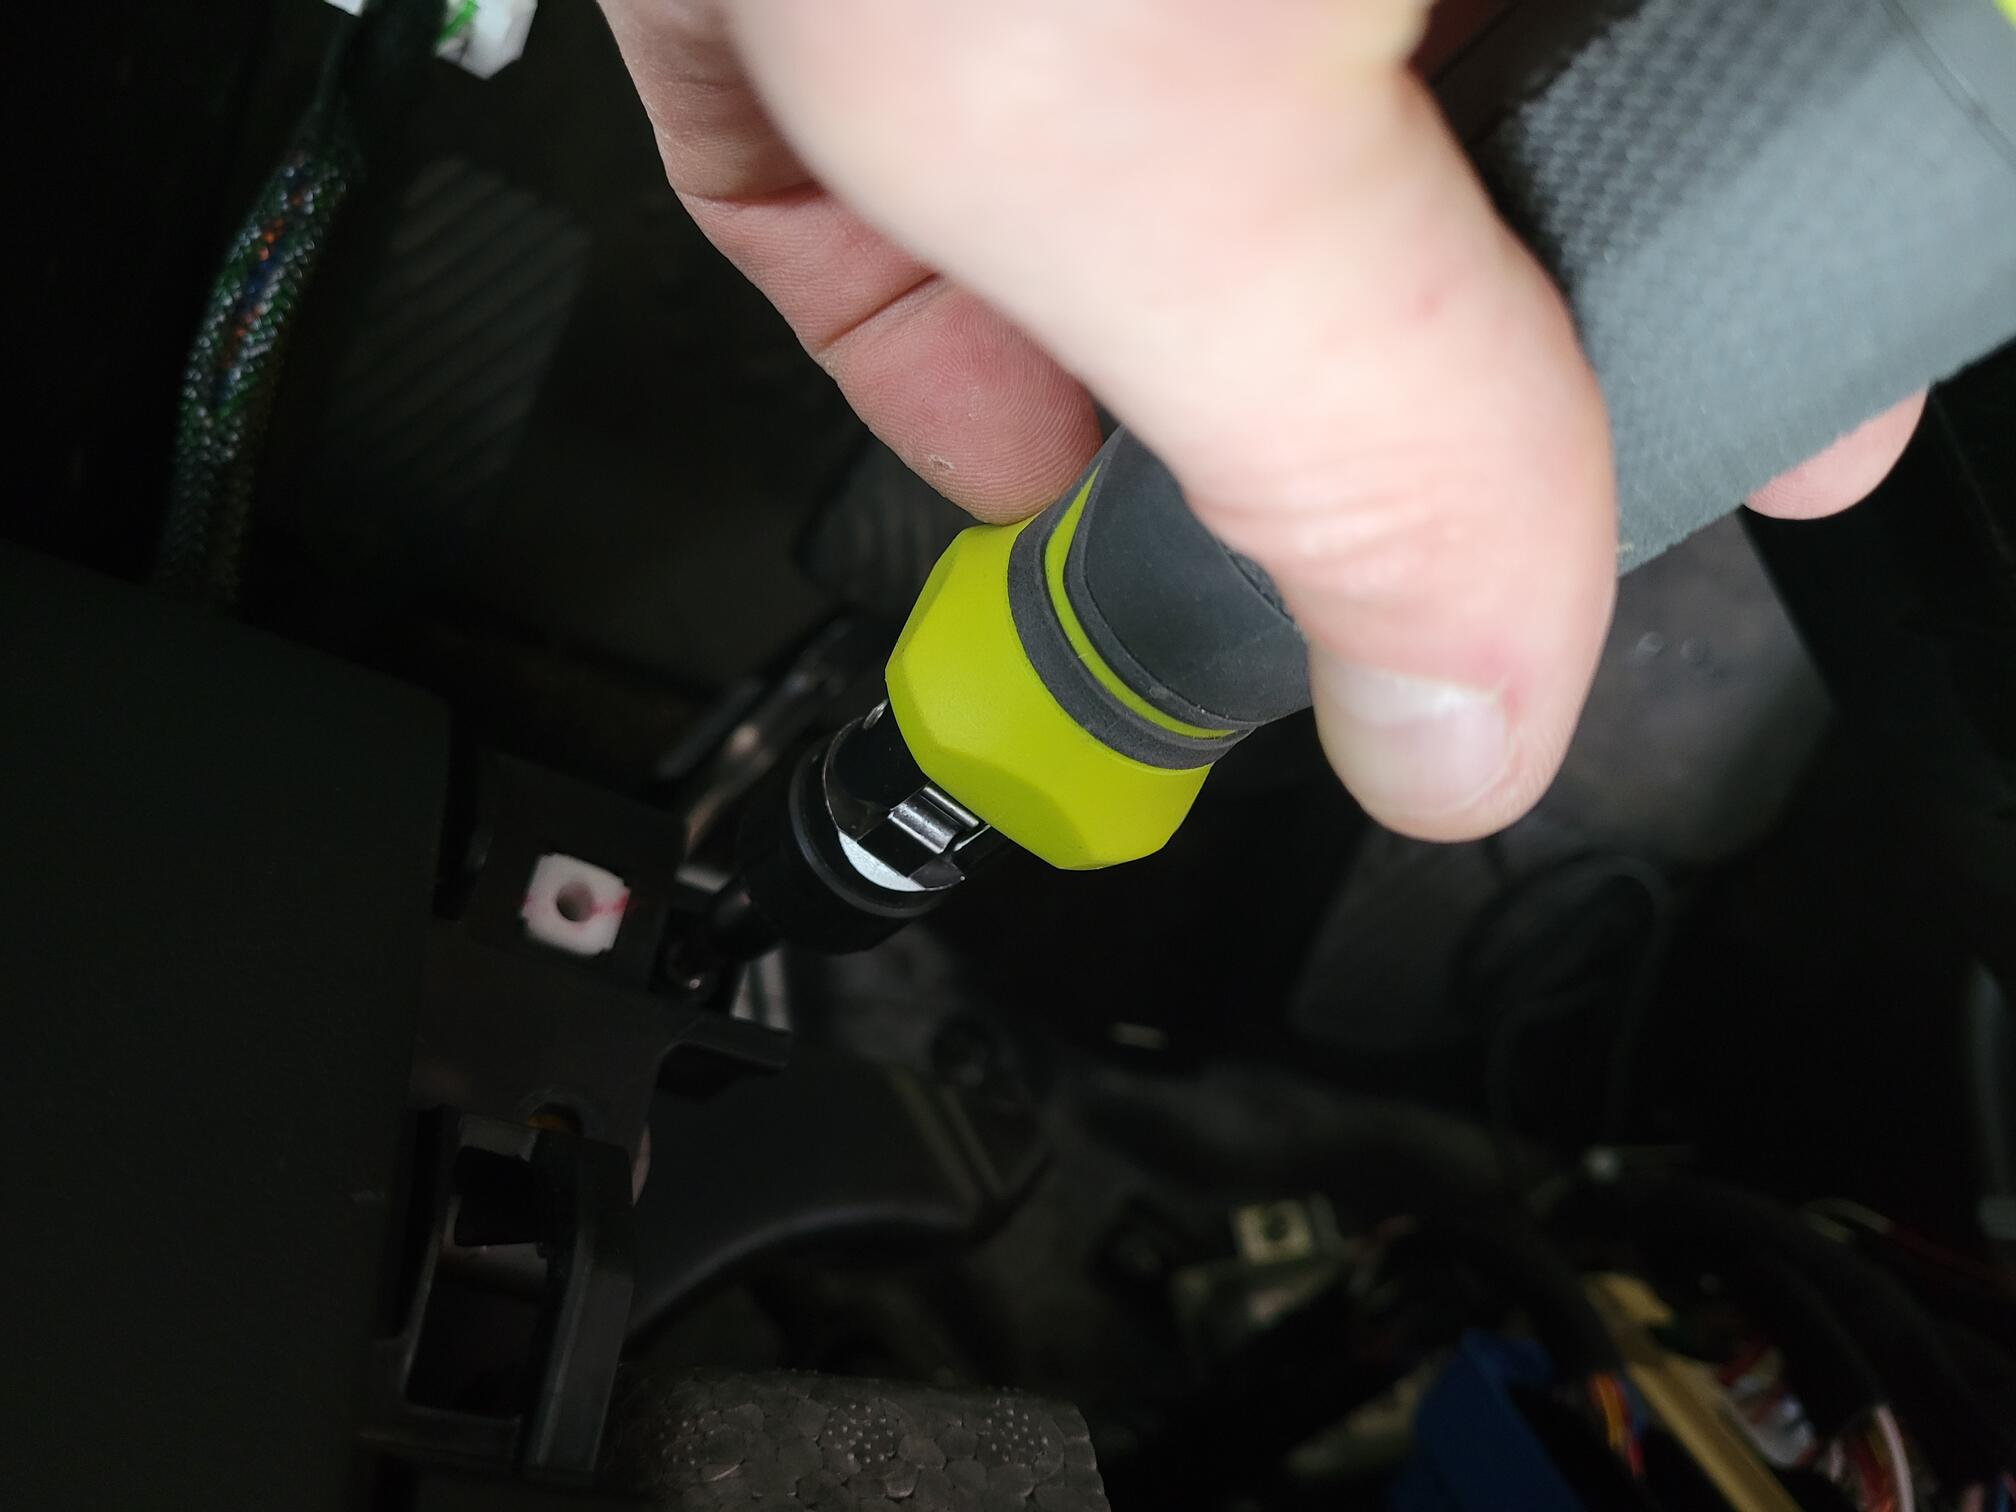
\includegraphics[height=1.5in,angle=180]{photos/crash_pad_center_ll_screw.jpg} } 
  \subfloat[]{\label{subfig:trimsteps:cpg_r_screw}
  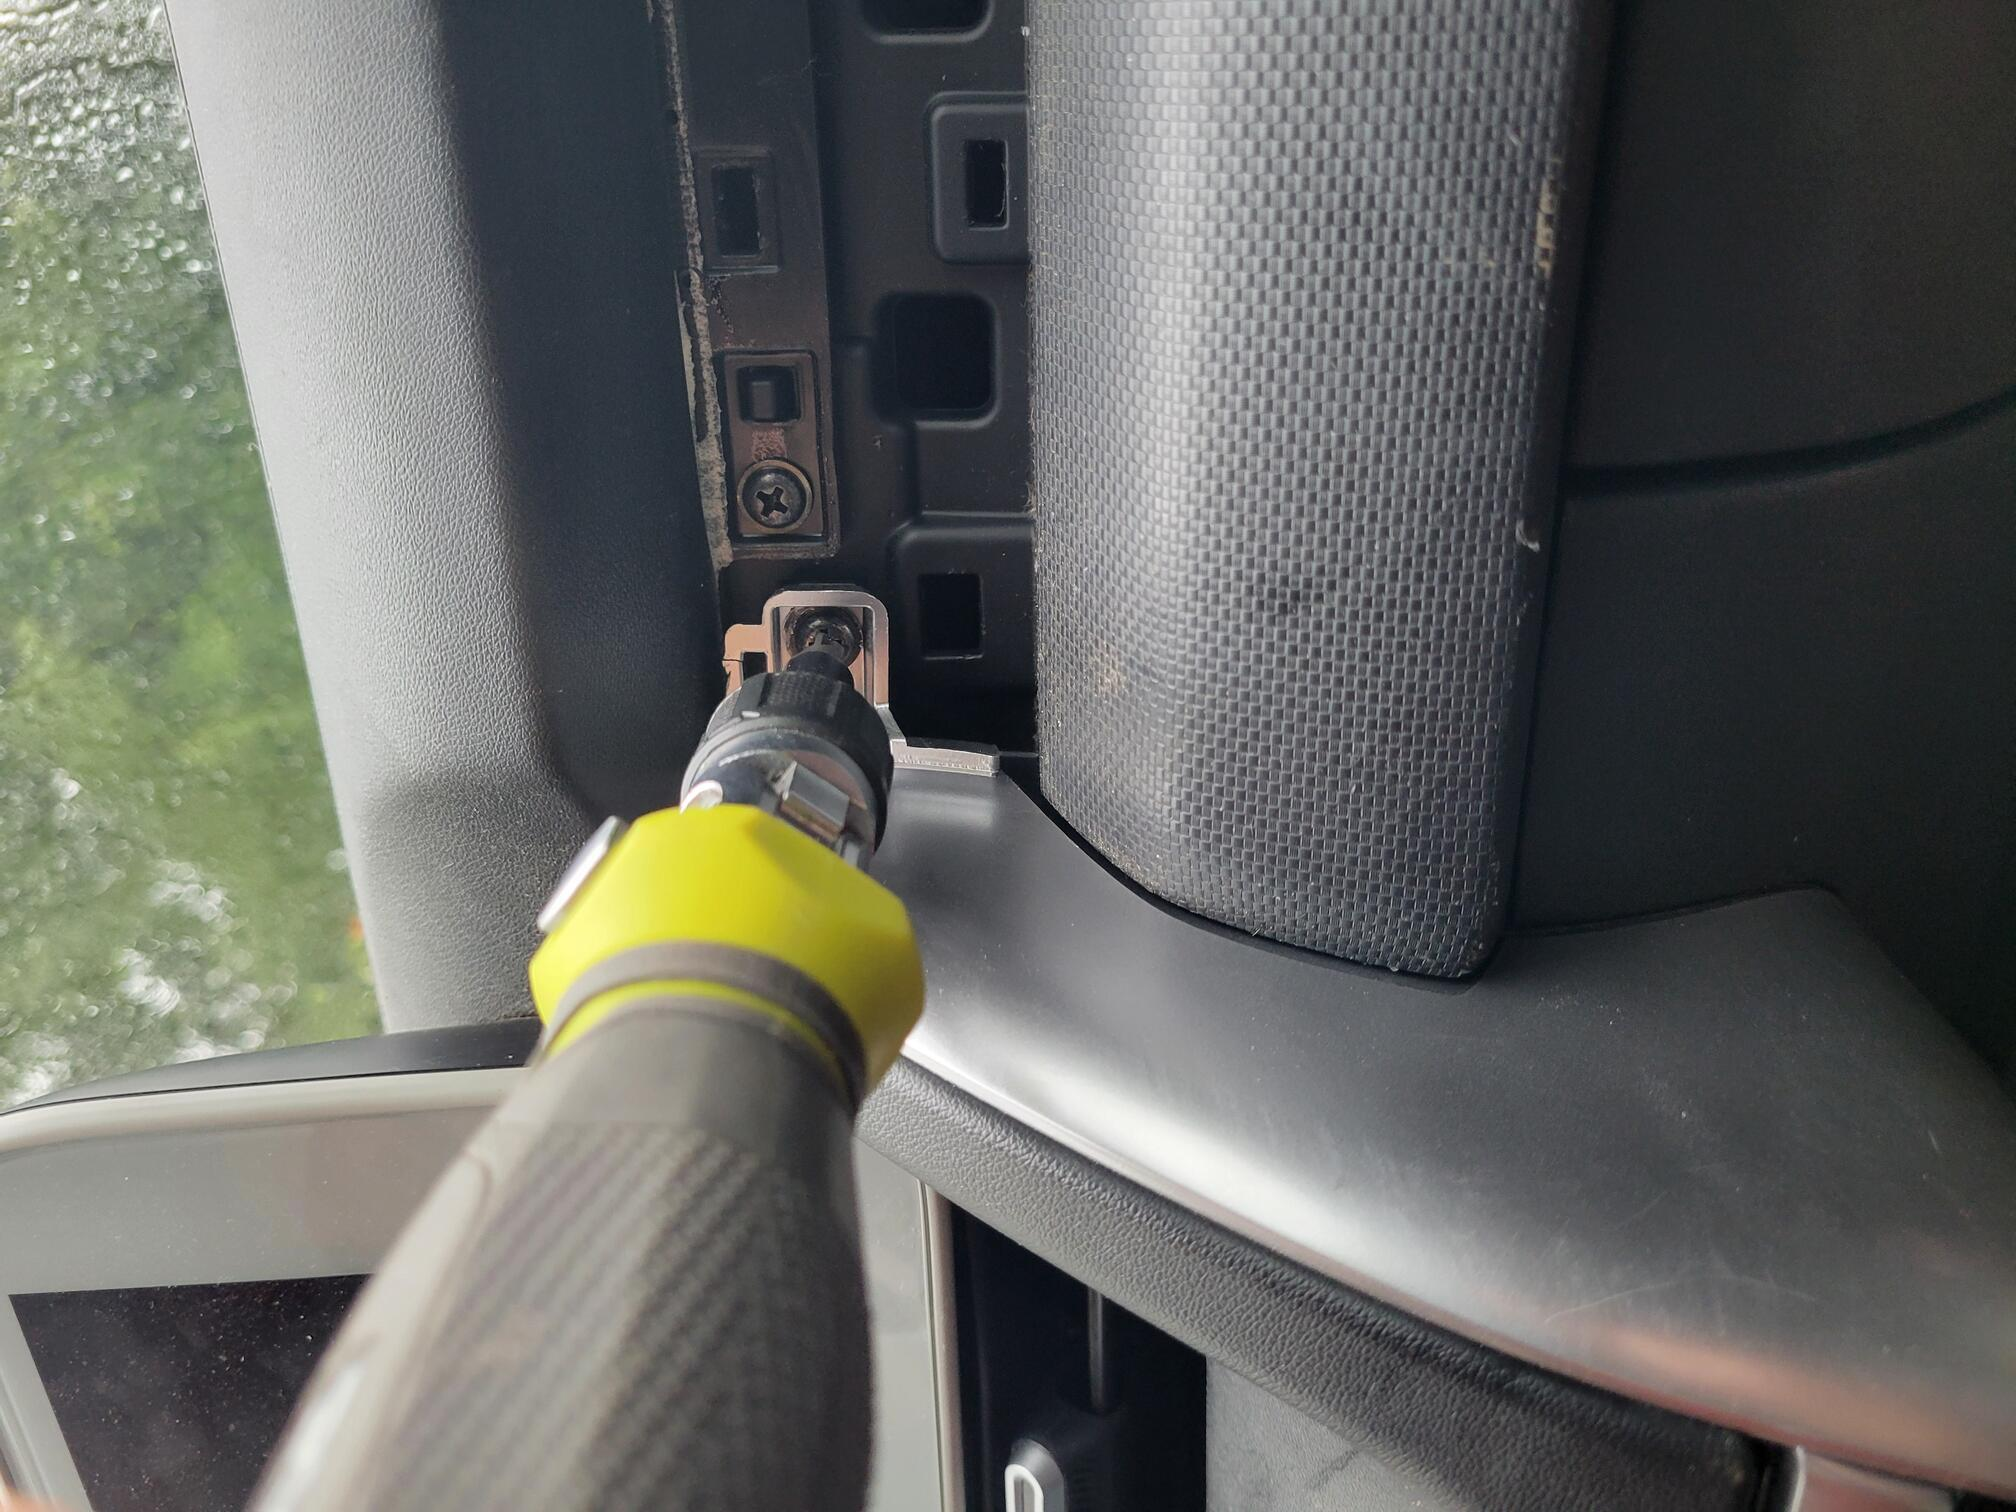
\includegraphics[width=1.5in,angle=-90]{photos/crash_pad_garnish_r_screw.jpg} }  \\
  \subfloat[]{\label{subfig:trimsteps:keyboard_l_screw}
  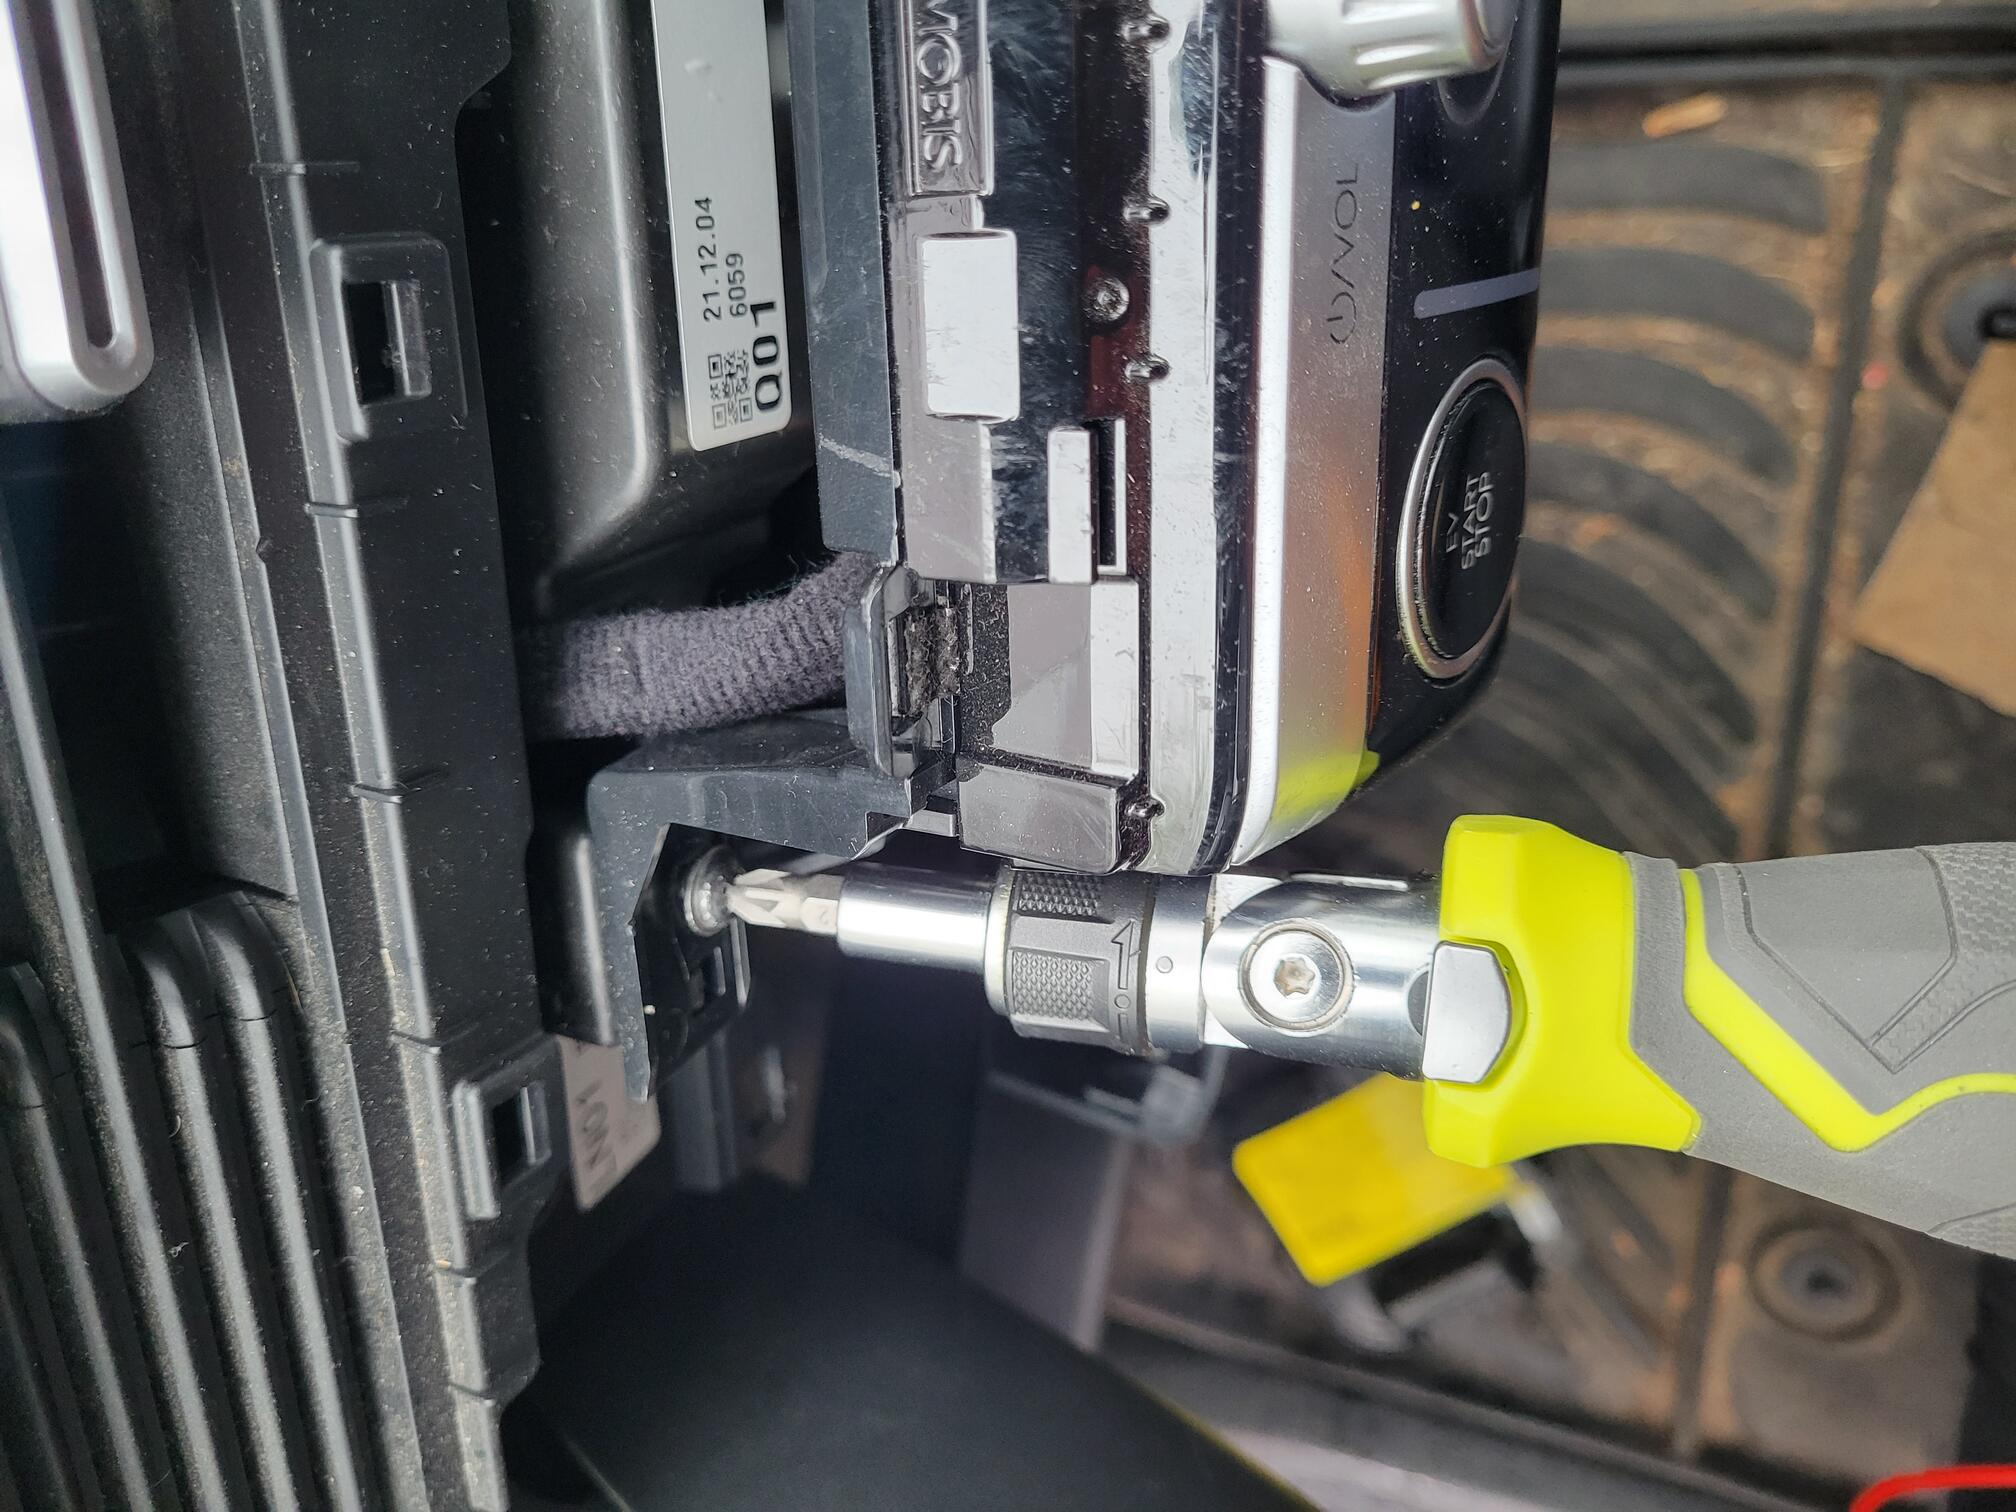
\includegraphics[height=1.5in,angle=180]{photos/keyboard_left_screw.jpg} } 
  \subfloat[]{\label{subfig:trimsteps:keyboard_ur_screw}
  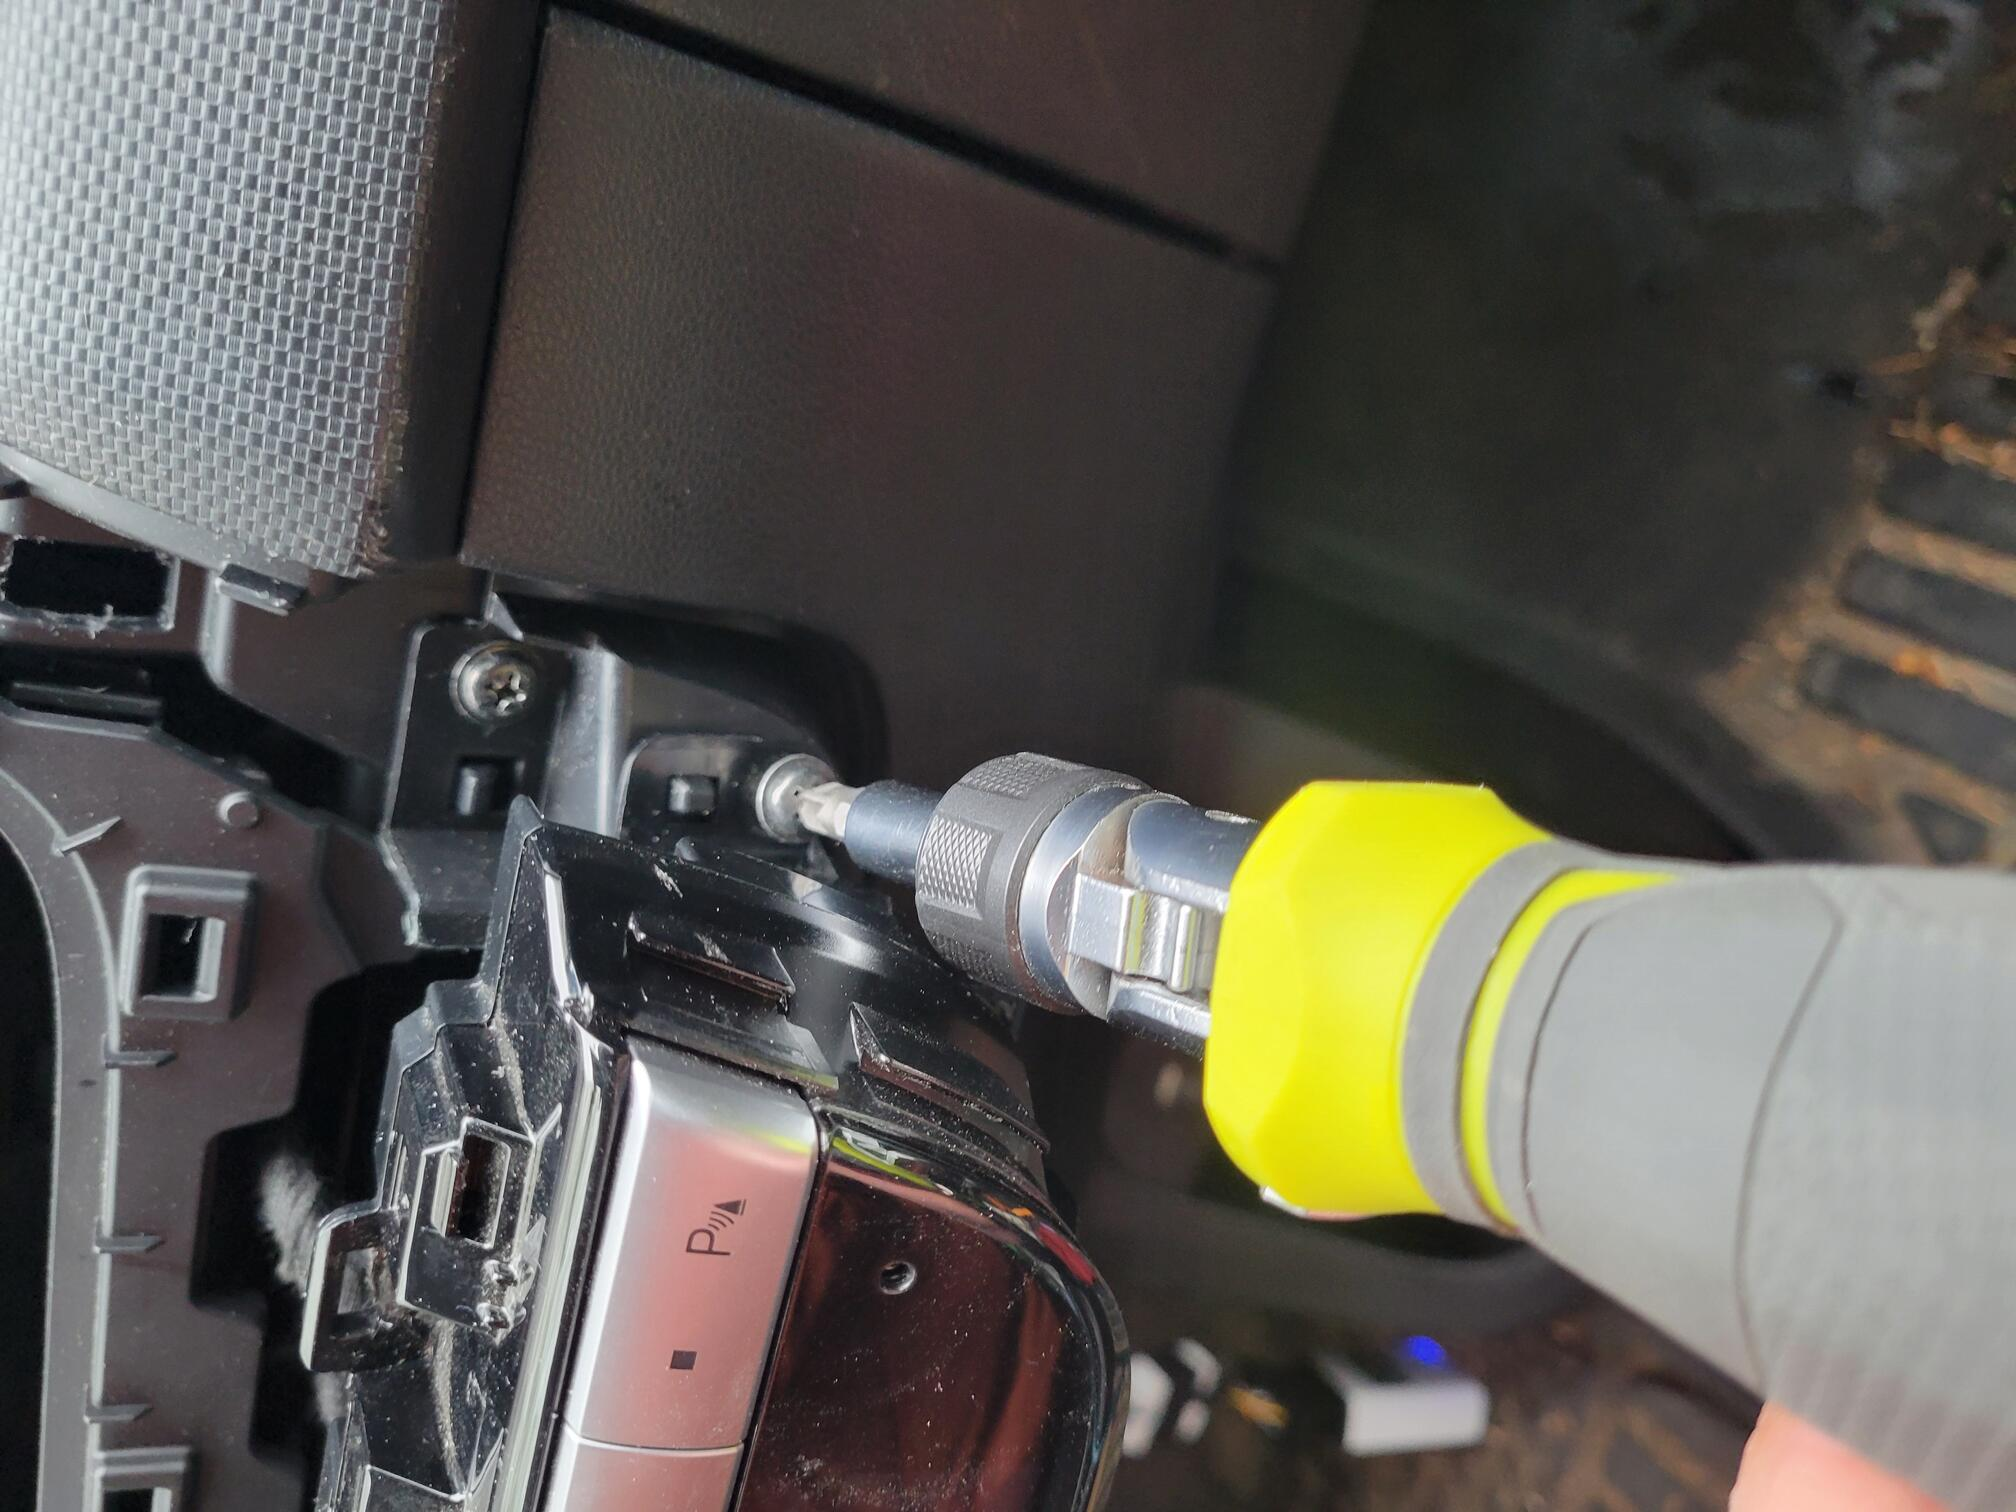
\includegraphics[width=1.5in,angle=-90]{photos/keyboard_ur_screw.jpg} } 
  \subfloat[]{\label{subfig:trimsteps:keyboard_ll_screw}
  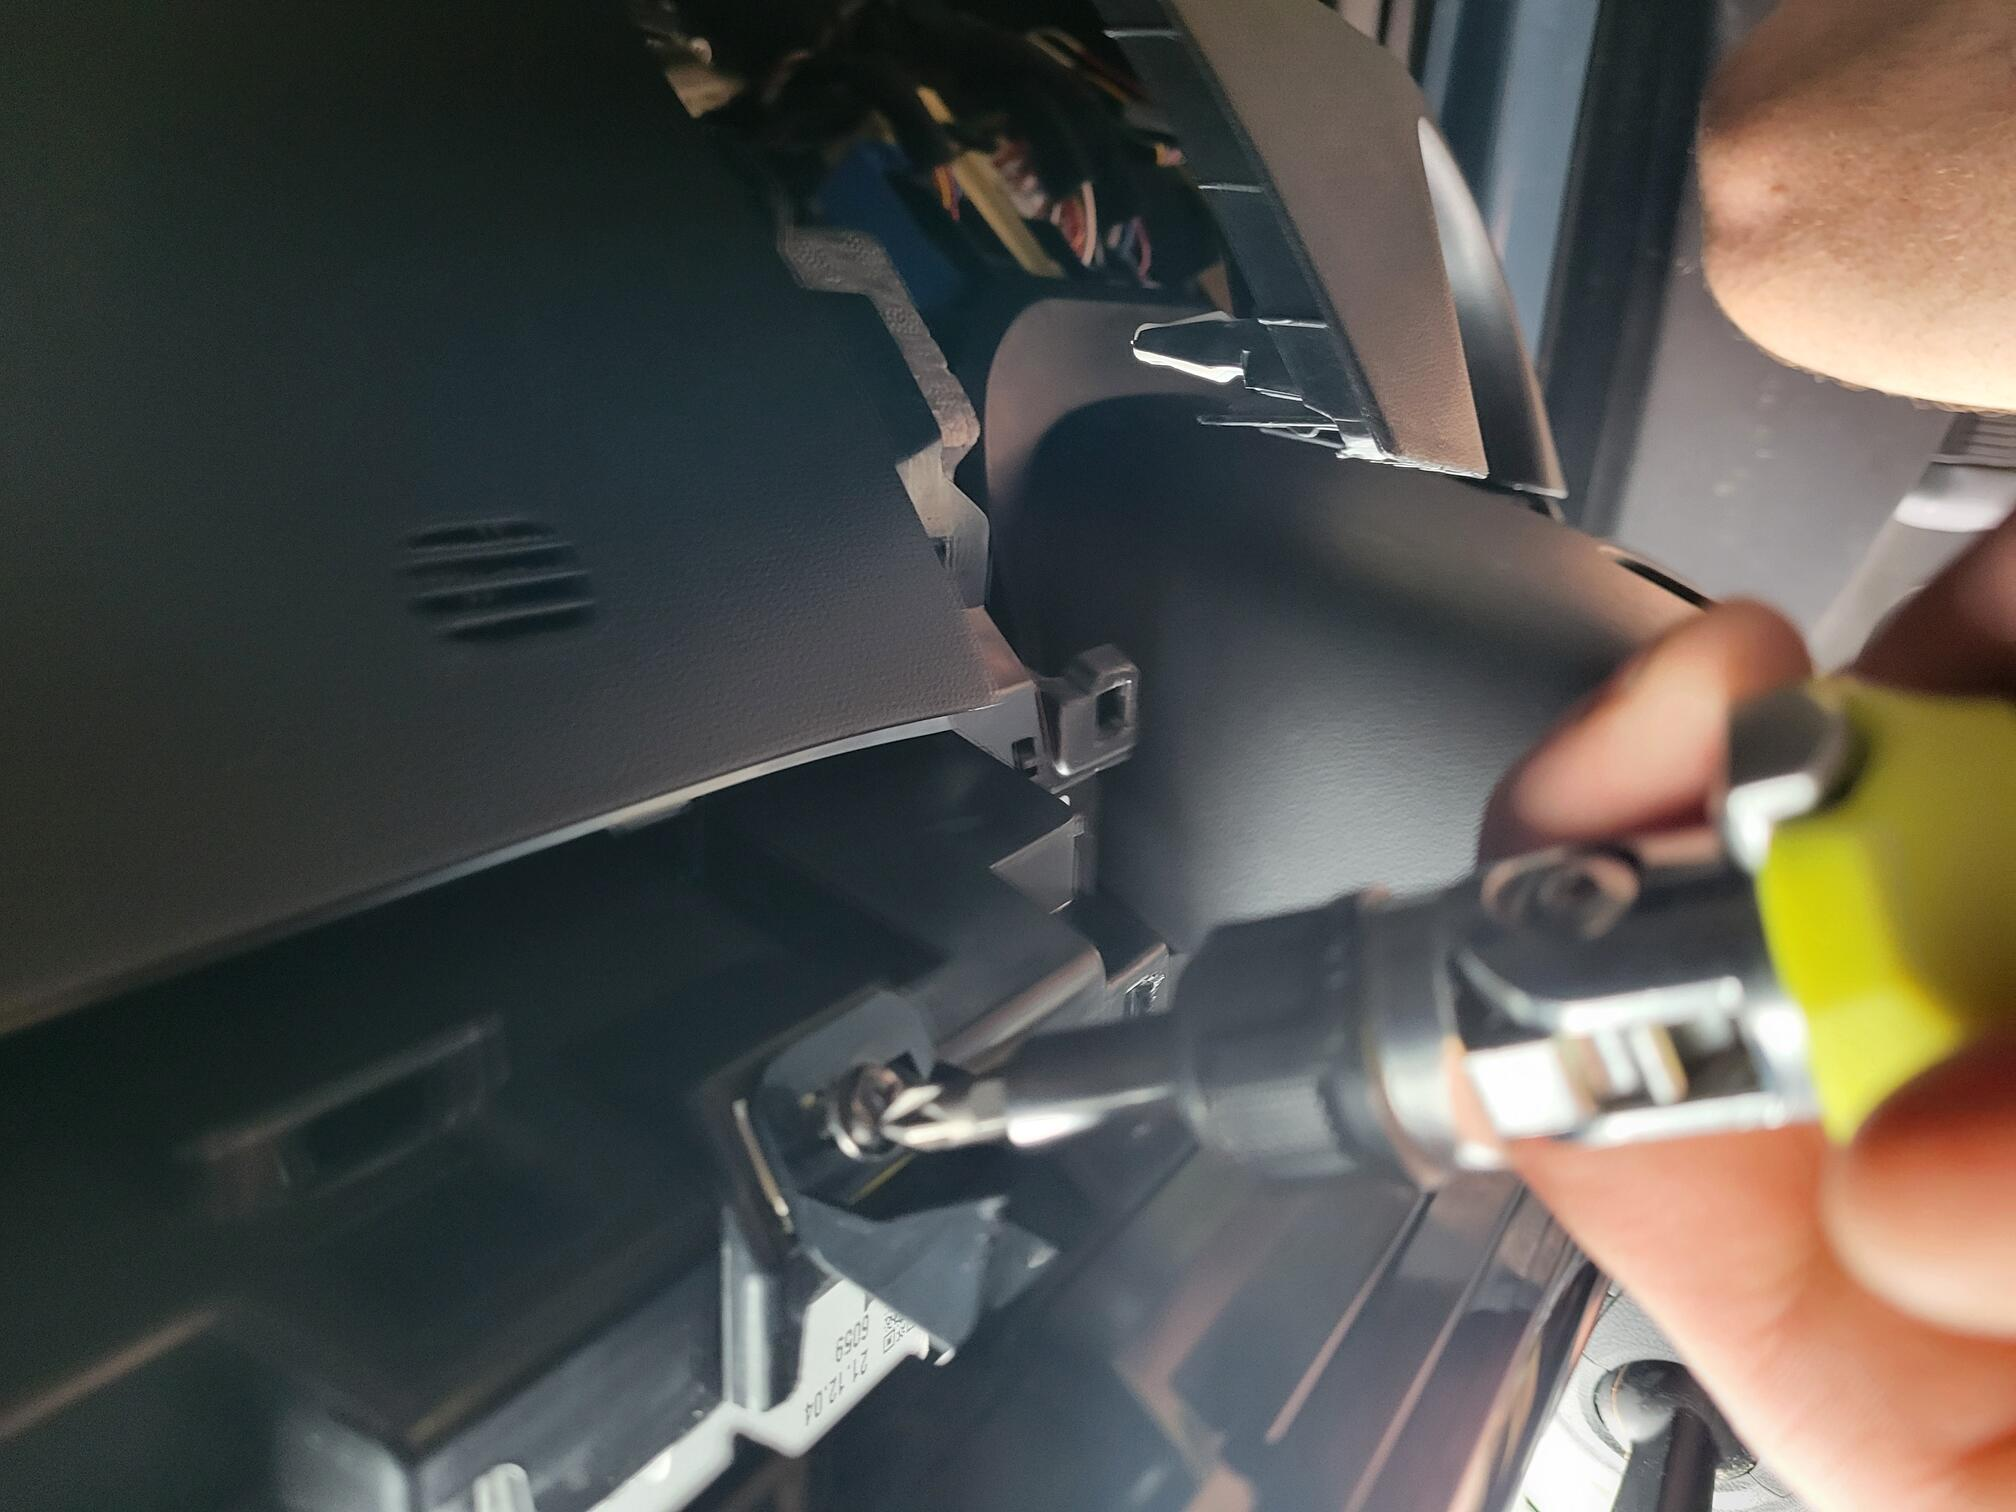
\includegraphics[height=1.5in,angle=180]{photos/keyboard_ll_screw.jpg} }  \\
  \subfloat[]{\label{subfig:trimsteps:keyboard_lr_screw}
  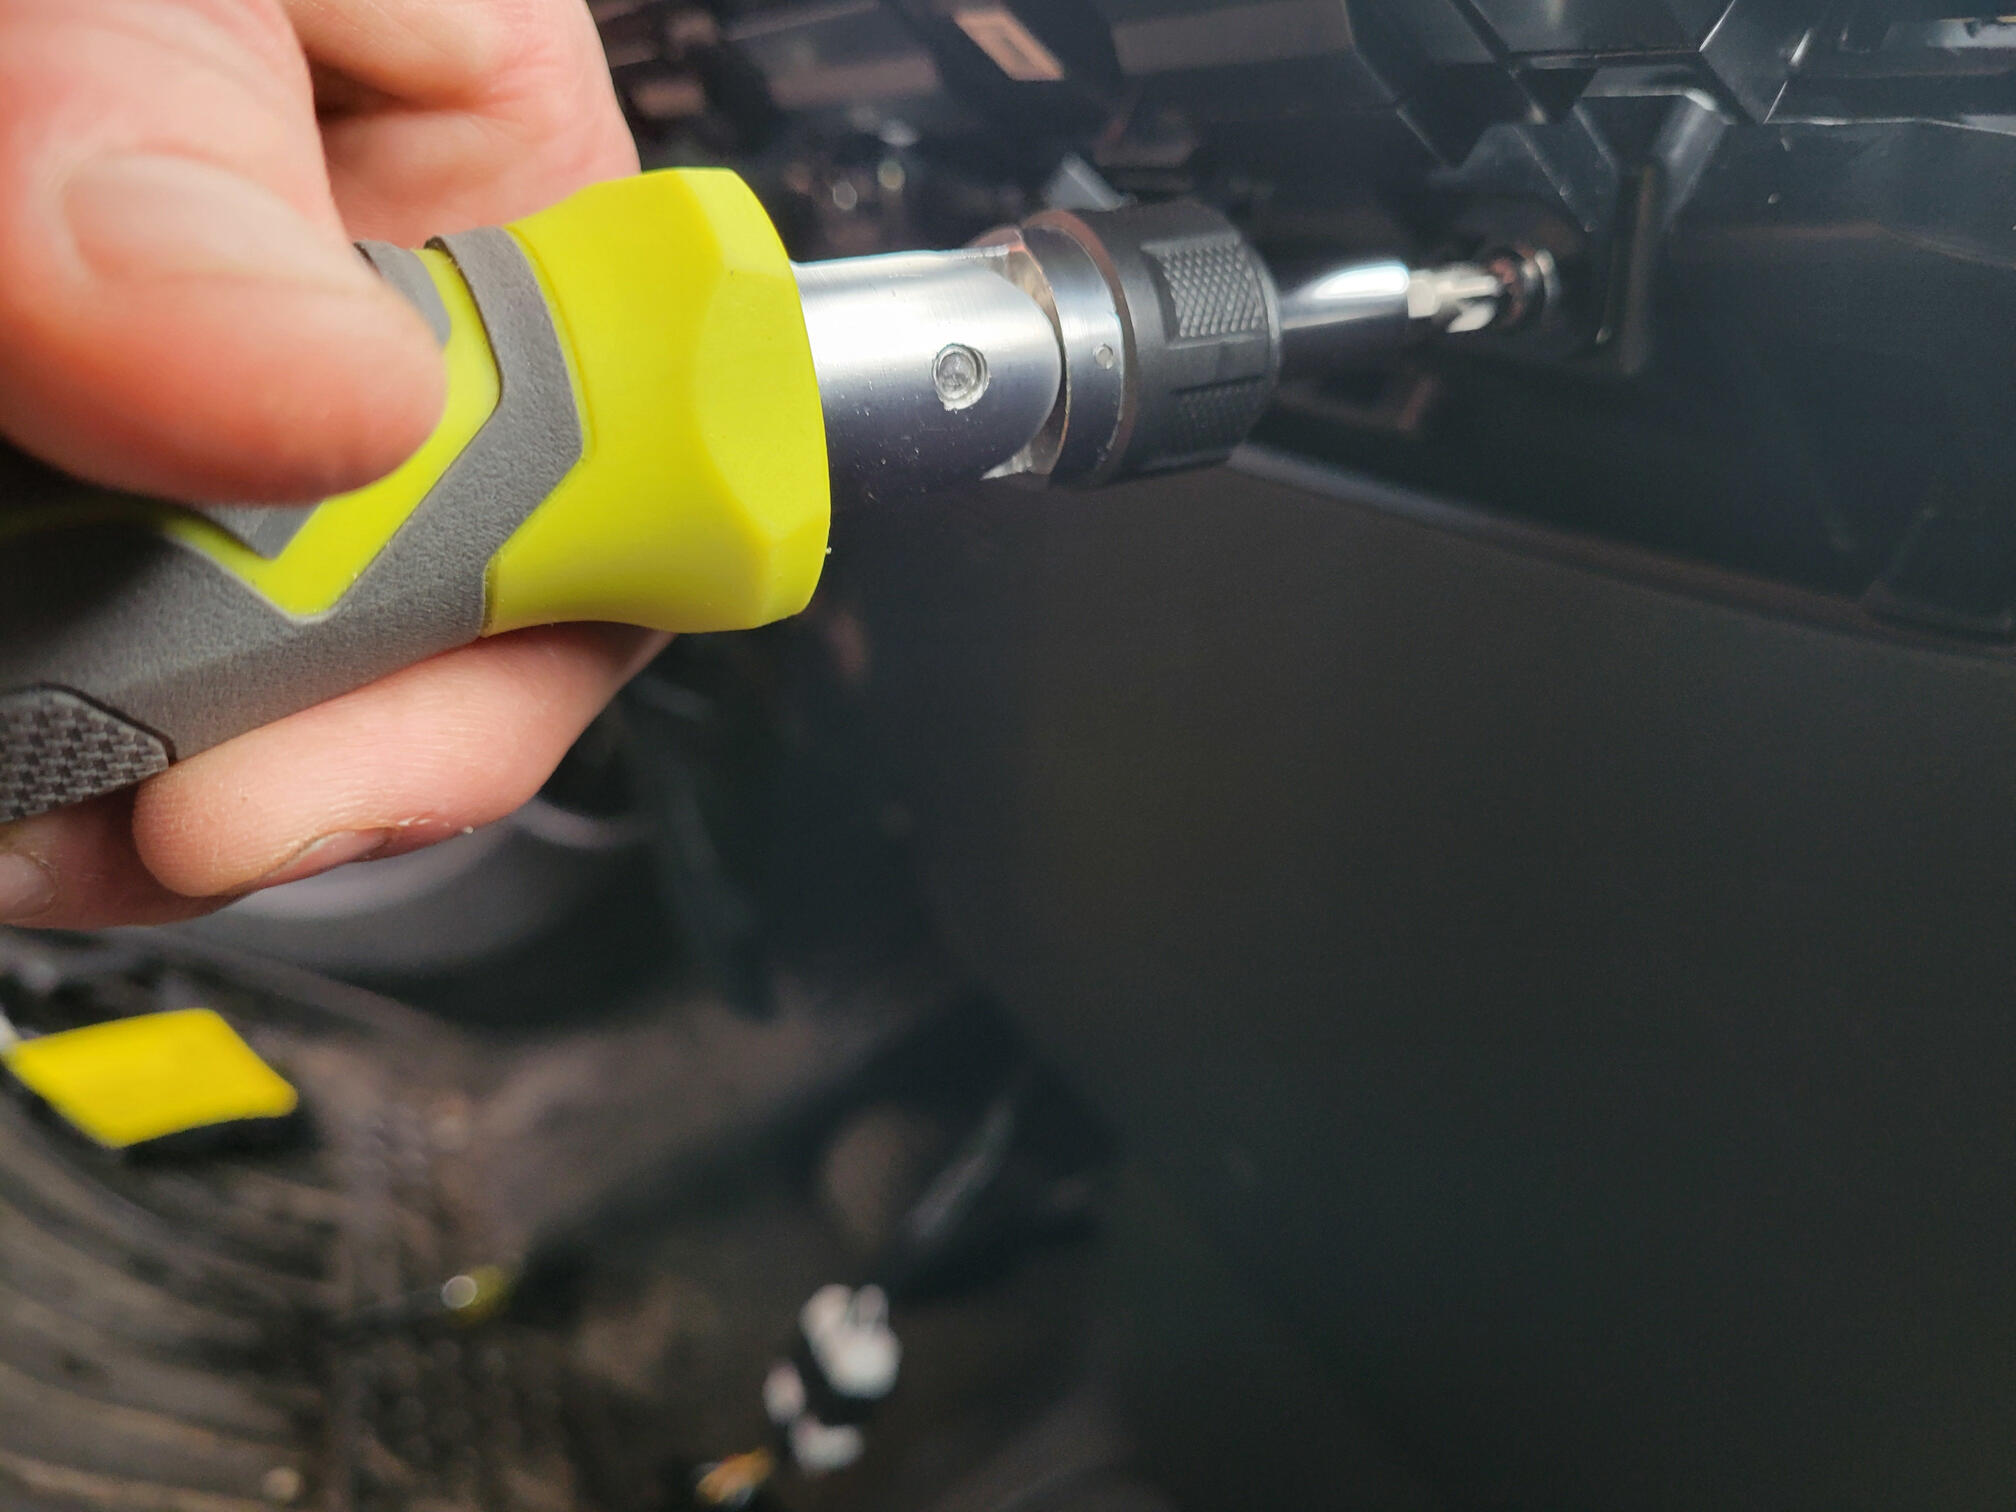
\includegraphics[height=1.5in,angle=0]{photos/keyboard_lr_screw.jpg} } 
  \subfloat[]{\label{subfig:trimsteps:remove_keyboard}
  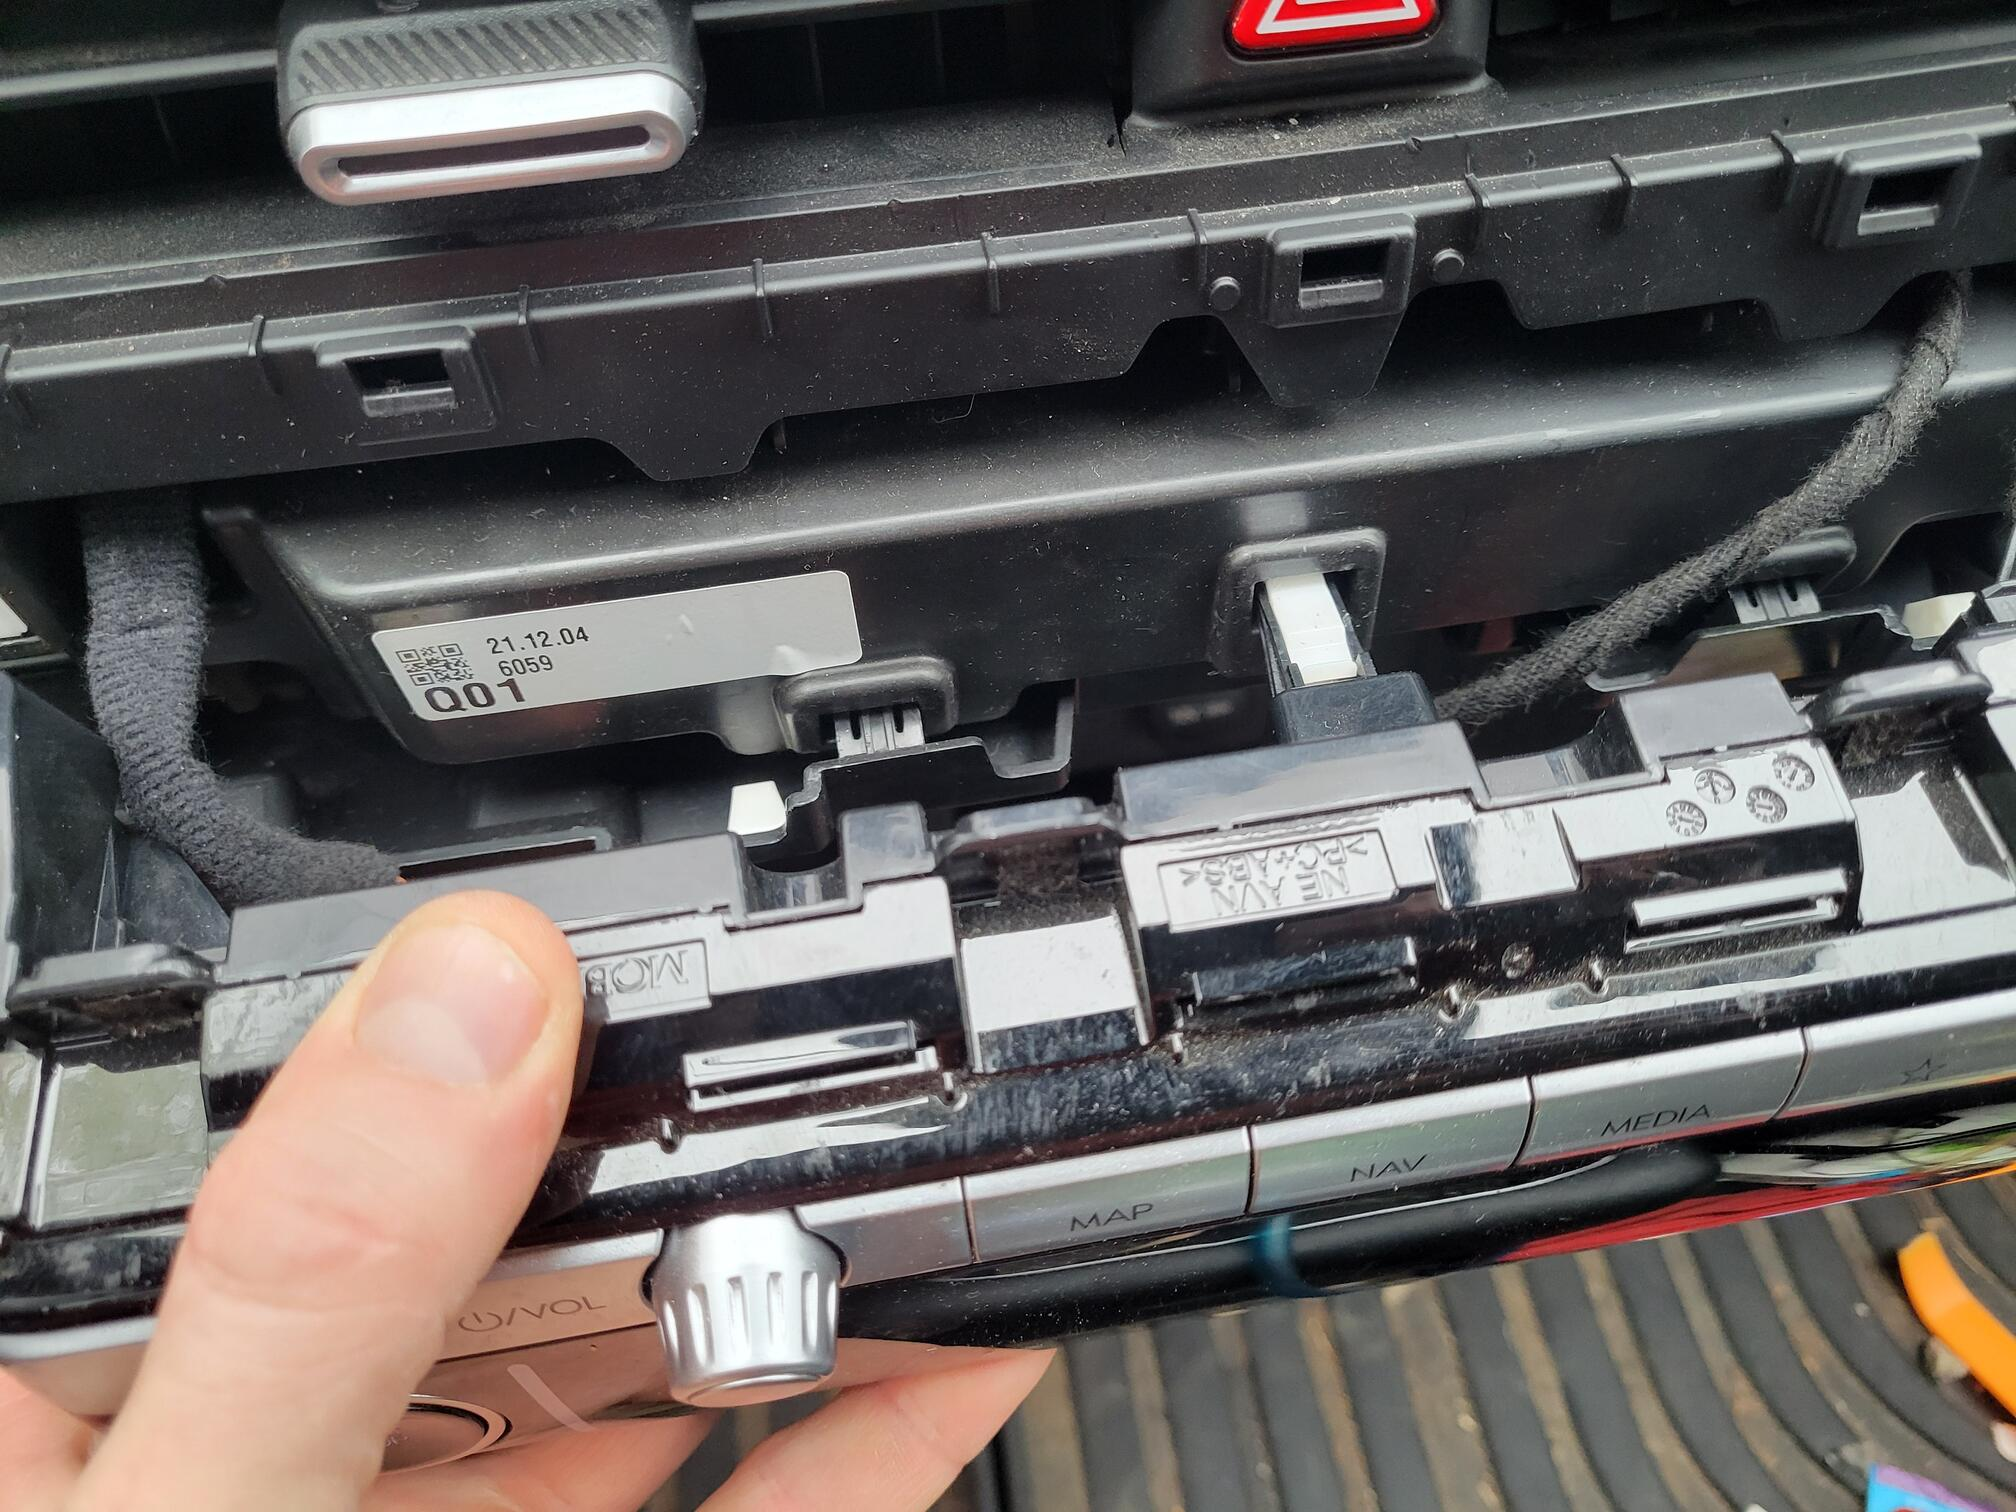
\includegraphics[height=1.5in,angle=0]{photos/remove_keyboard.jpg} }  \\
  \subfloat[]{\label{subfig:trimsteps:cpc_urscrew}
  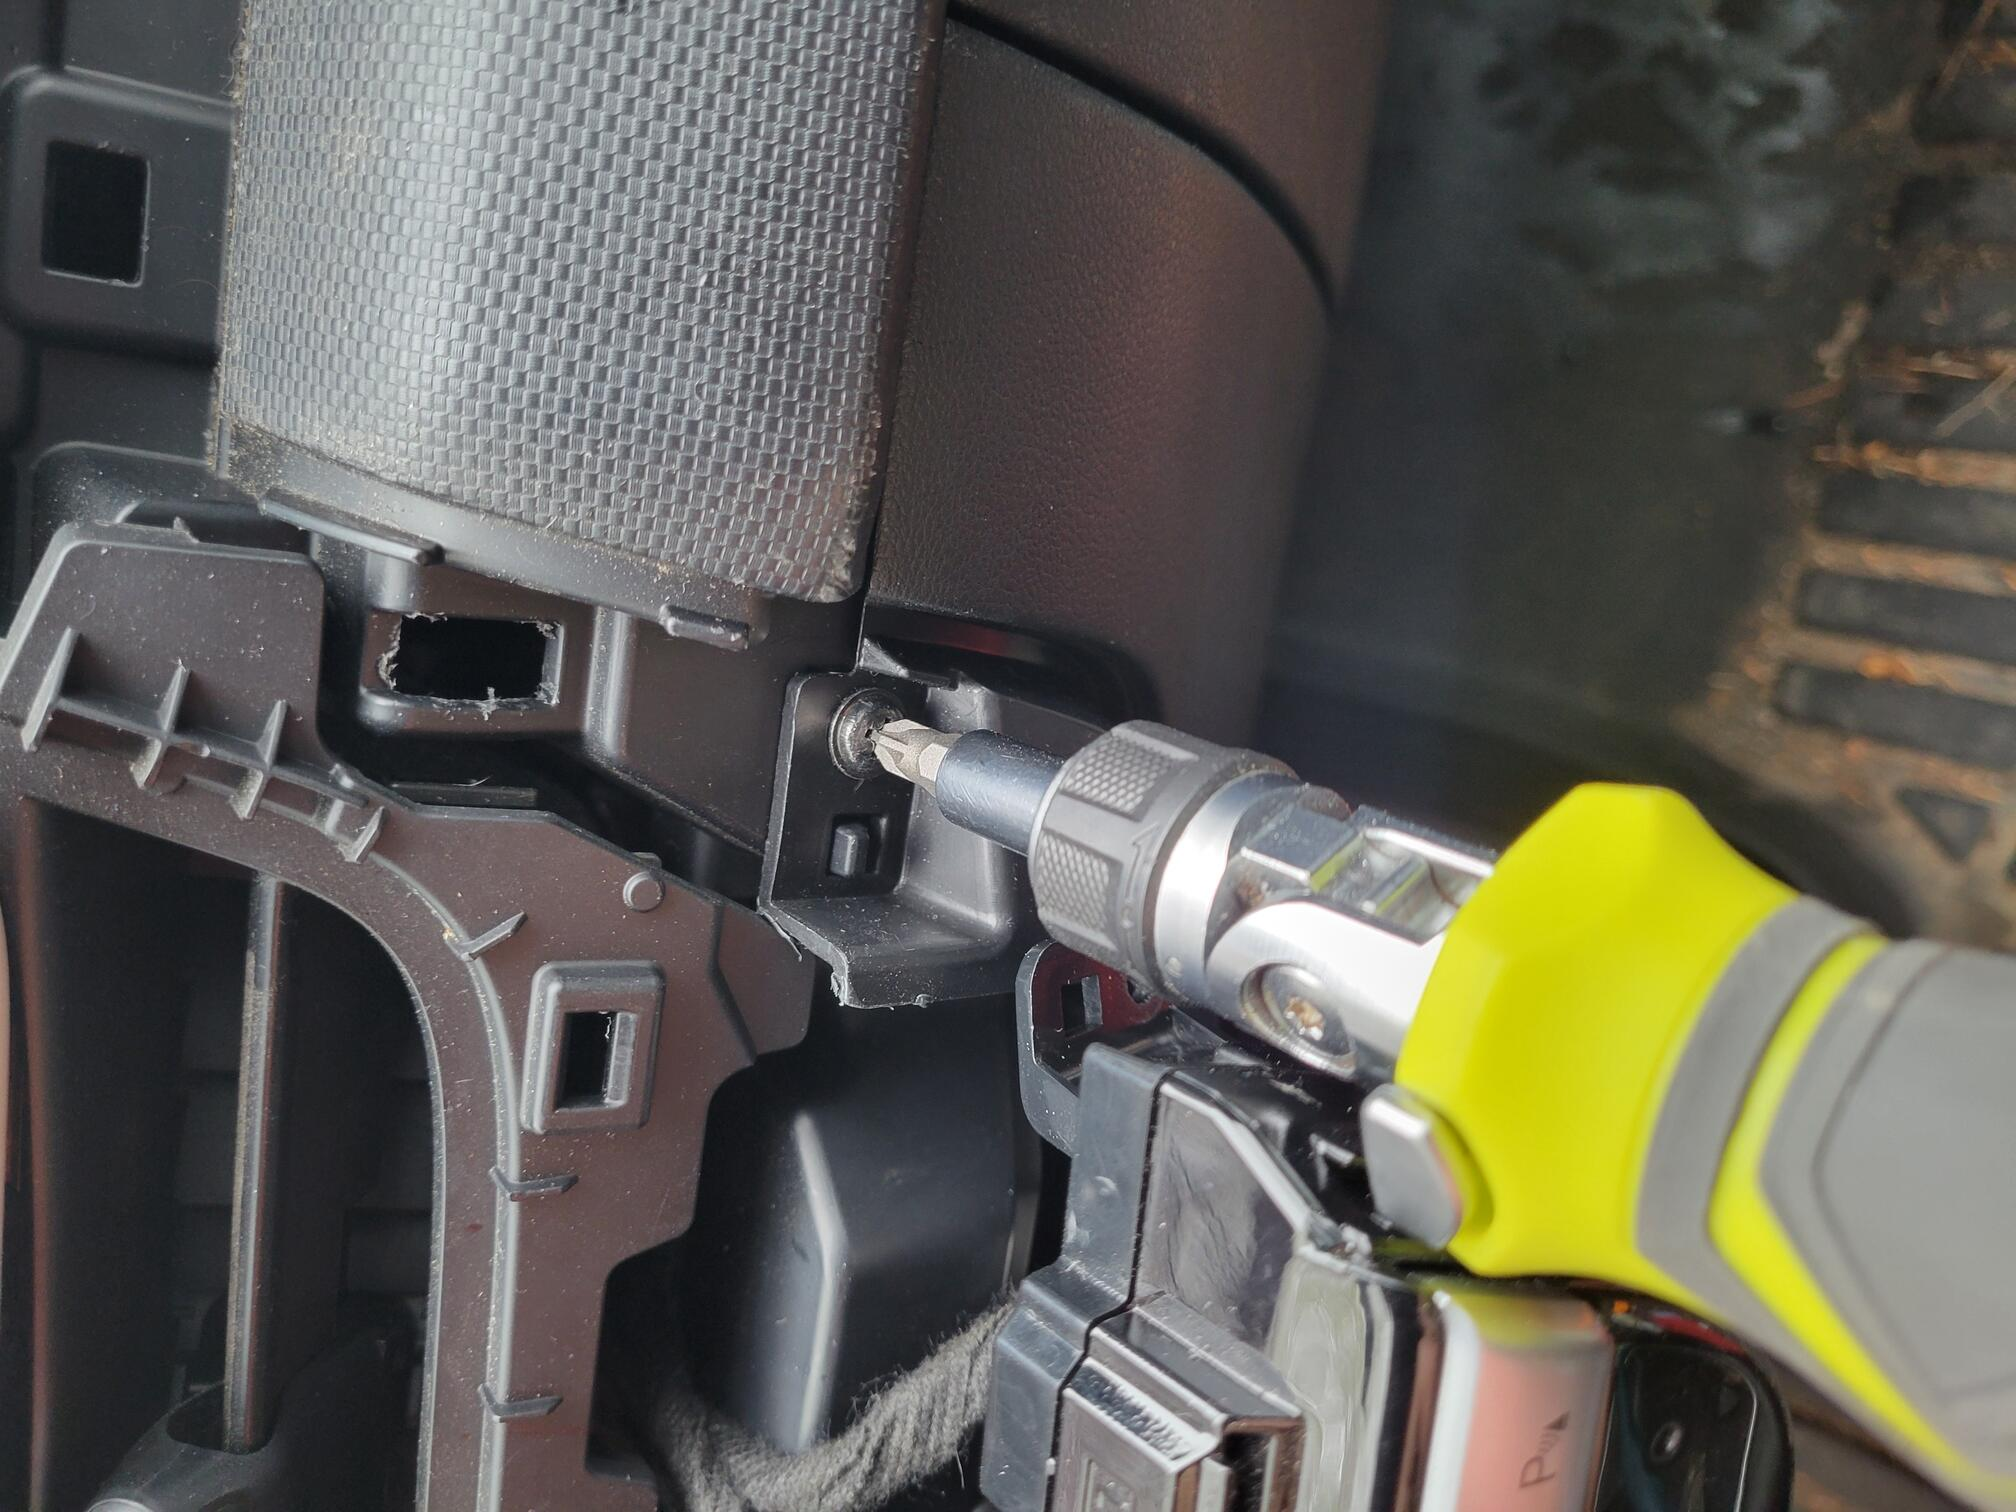
\includegraphics[width=1.5in,angle=-90]{photos/crash_pad_center_ur_screw.jpg} }  
  \subfloat[]{\label{subfig:trimsteps:cpc_ulscrew}
  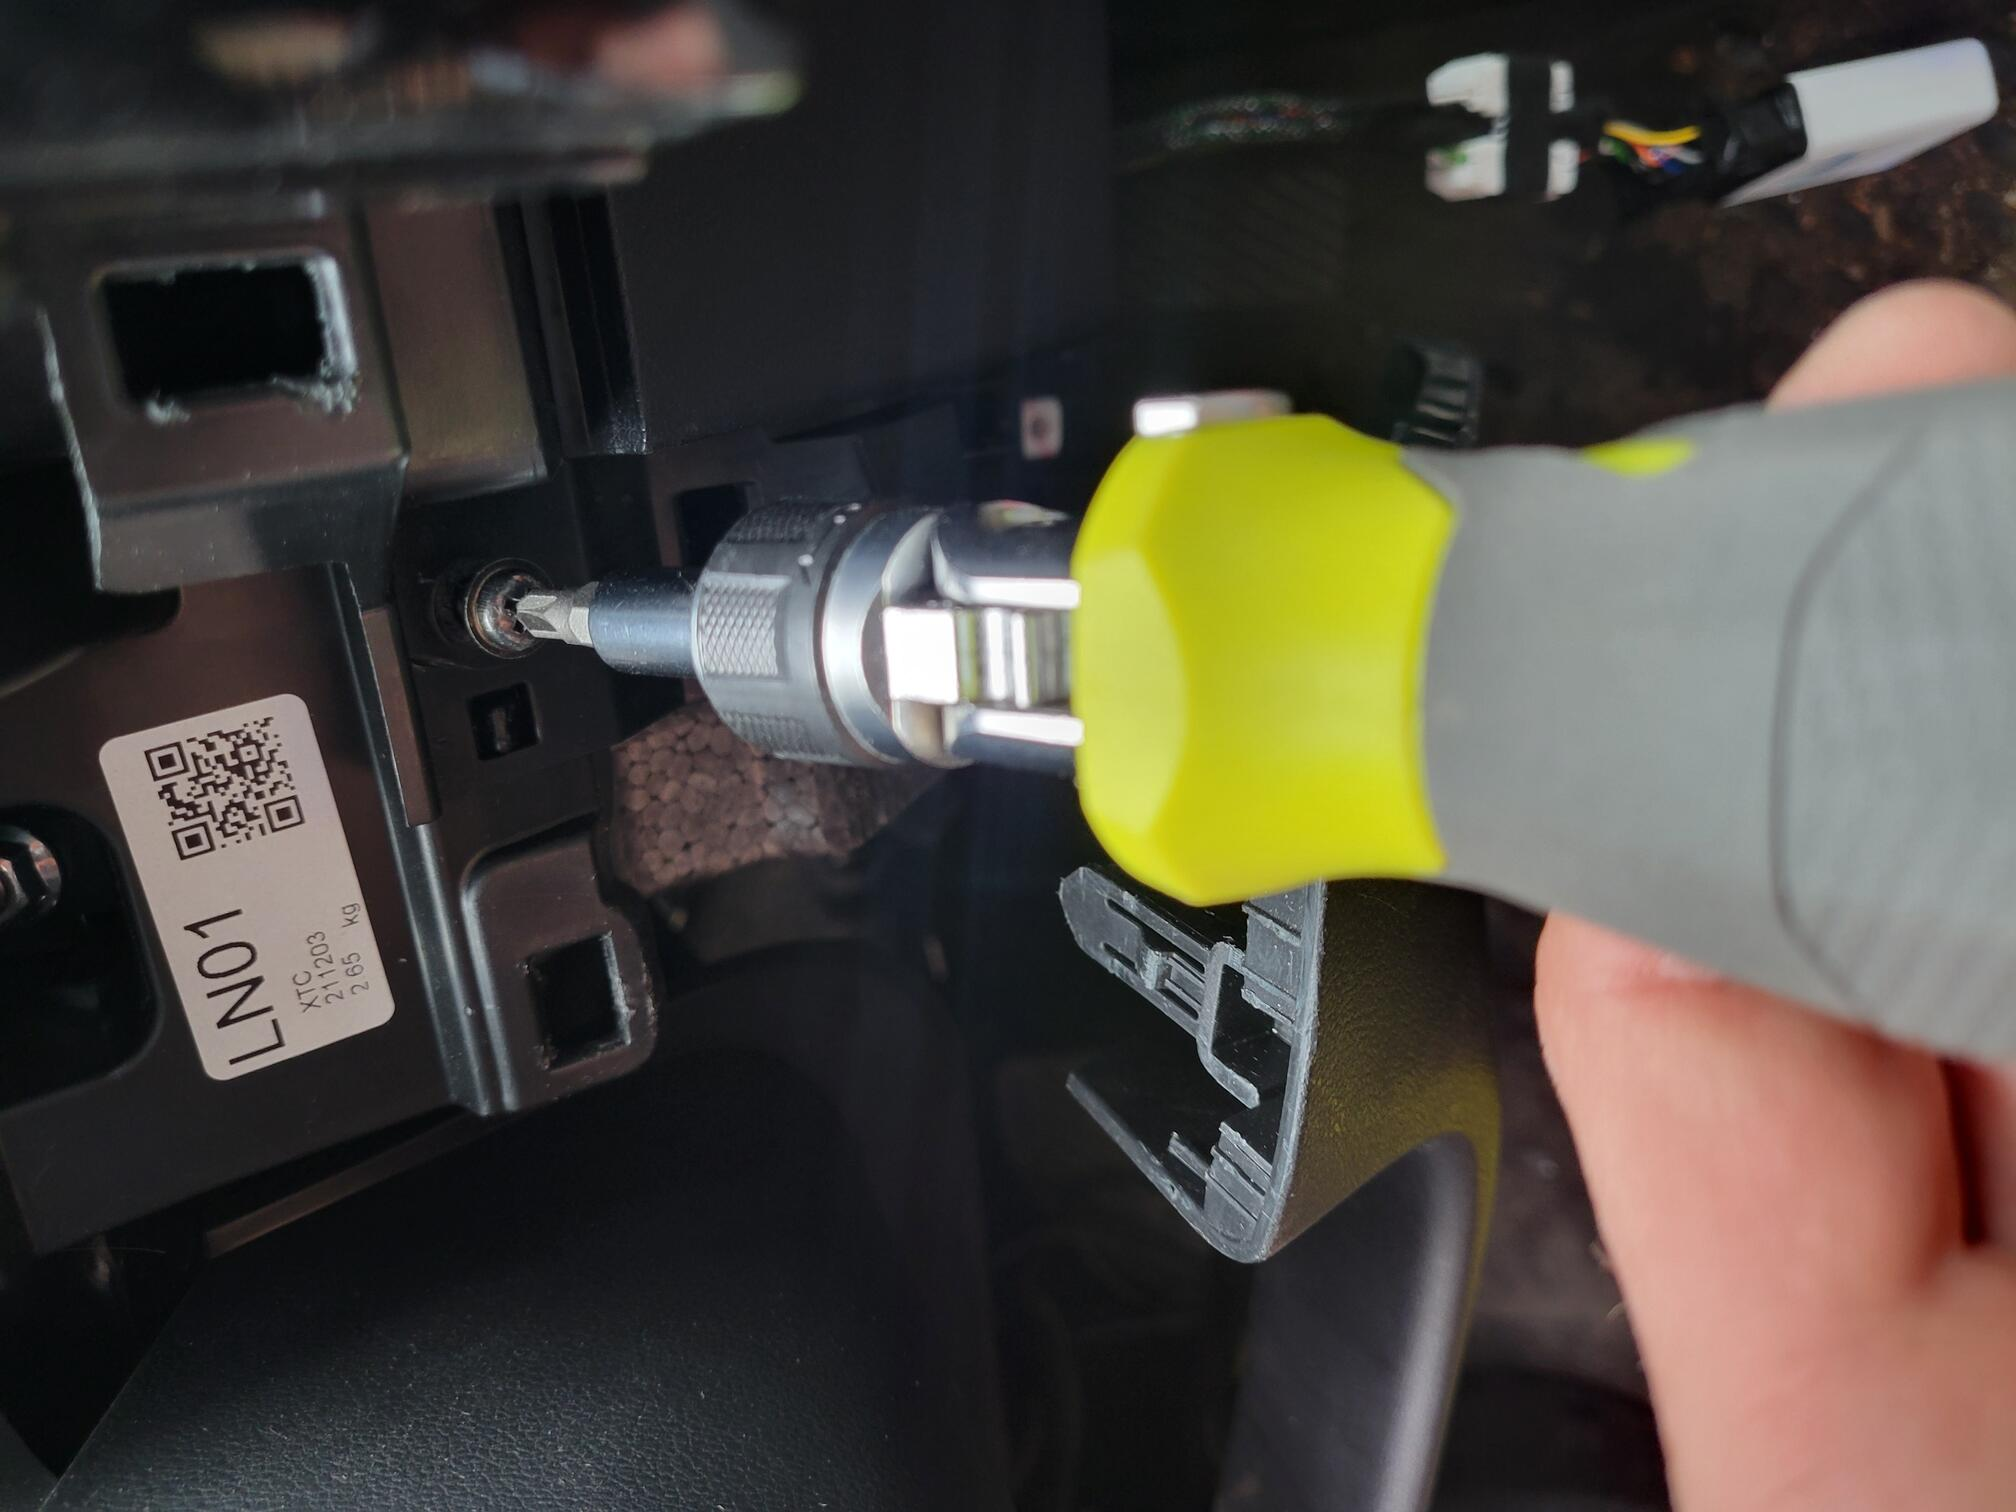
\includegraphics[width=1.5in,angle=-90]{photos/crash_pad_center_ul_screw.jpg} } 
   \caption{(a) Removing screw in crash pad lower. (b) Removing screw behind crash pad lower. (c) Removing screw holding in crash pad garnish. (d) Removing AVN keyboard left screw. (e) Removing AVN keyboard right screw. (f) Removing AVN keyboard lower left screw. (g) Removing AVN keyboard lower right screw. (h) Removing AVN keyboard. (i) Removing crash pad center screw that was blocked by AVN keyboard. (j) Removing crash pad center screw that was behind crash pad garnish, left of the AVN keyboard. \label{fig:trimsteps}}
\end{figure}
\subsection{Option B: quick and dirty}
We only partially remove two trim panels with this approach:
\begin{enumerate}
  \item Crash pad lower
  \item Crash pad center
\end{enumerate}

Step-by-step instructions:
\begin{enumerate}
  \item Remove screw in crash pad lower (Figure \ref{subfig:trimsteps:lowerscrew})
  \item Pull off right half of crash pad lower using trim removal tool 
  \item While here, remove screw behind crash pad lower; this screw tends to remain captive, so you have to pull to confirm it's out (Figure \ref{subfig:trimsteps:cpc_llscrew})
  \item Pull out the bottom of crash pad center
  \item You can now access the head unit from underneath crash pad center
\end{enumerate}

\section{Step 3: Harness Connection} \label{sect:2}
This step covers the installation of the harness into the head unit. 

Step-by-step instructions:
\begin{enumerate}
  \item Identify original grey female head unit connector (Figure \ref{subfig:harness:headunit})
  \item Remove it by squeezing the clip and pulling down (Figure \ref{subfig:harness:M05Bout})
  \item Insert the harness female side into the head unit (Figure \ref{subfig:harness:female})
  \item Insert the female connector you removed into the harness male side (Figure \ref{subfig:harness:harness_in})
\end{enumerate}

\begin{figure}[h]
  \subfloat[]{\label{subfig:harness:female}
  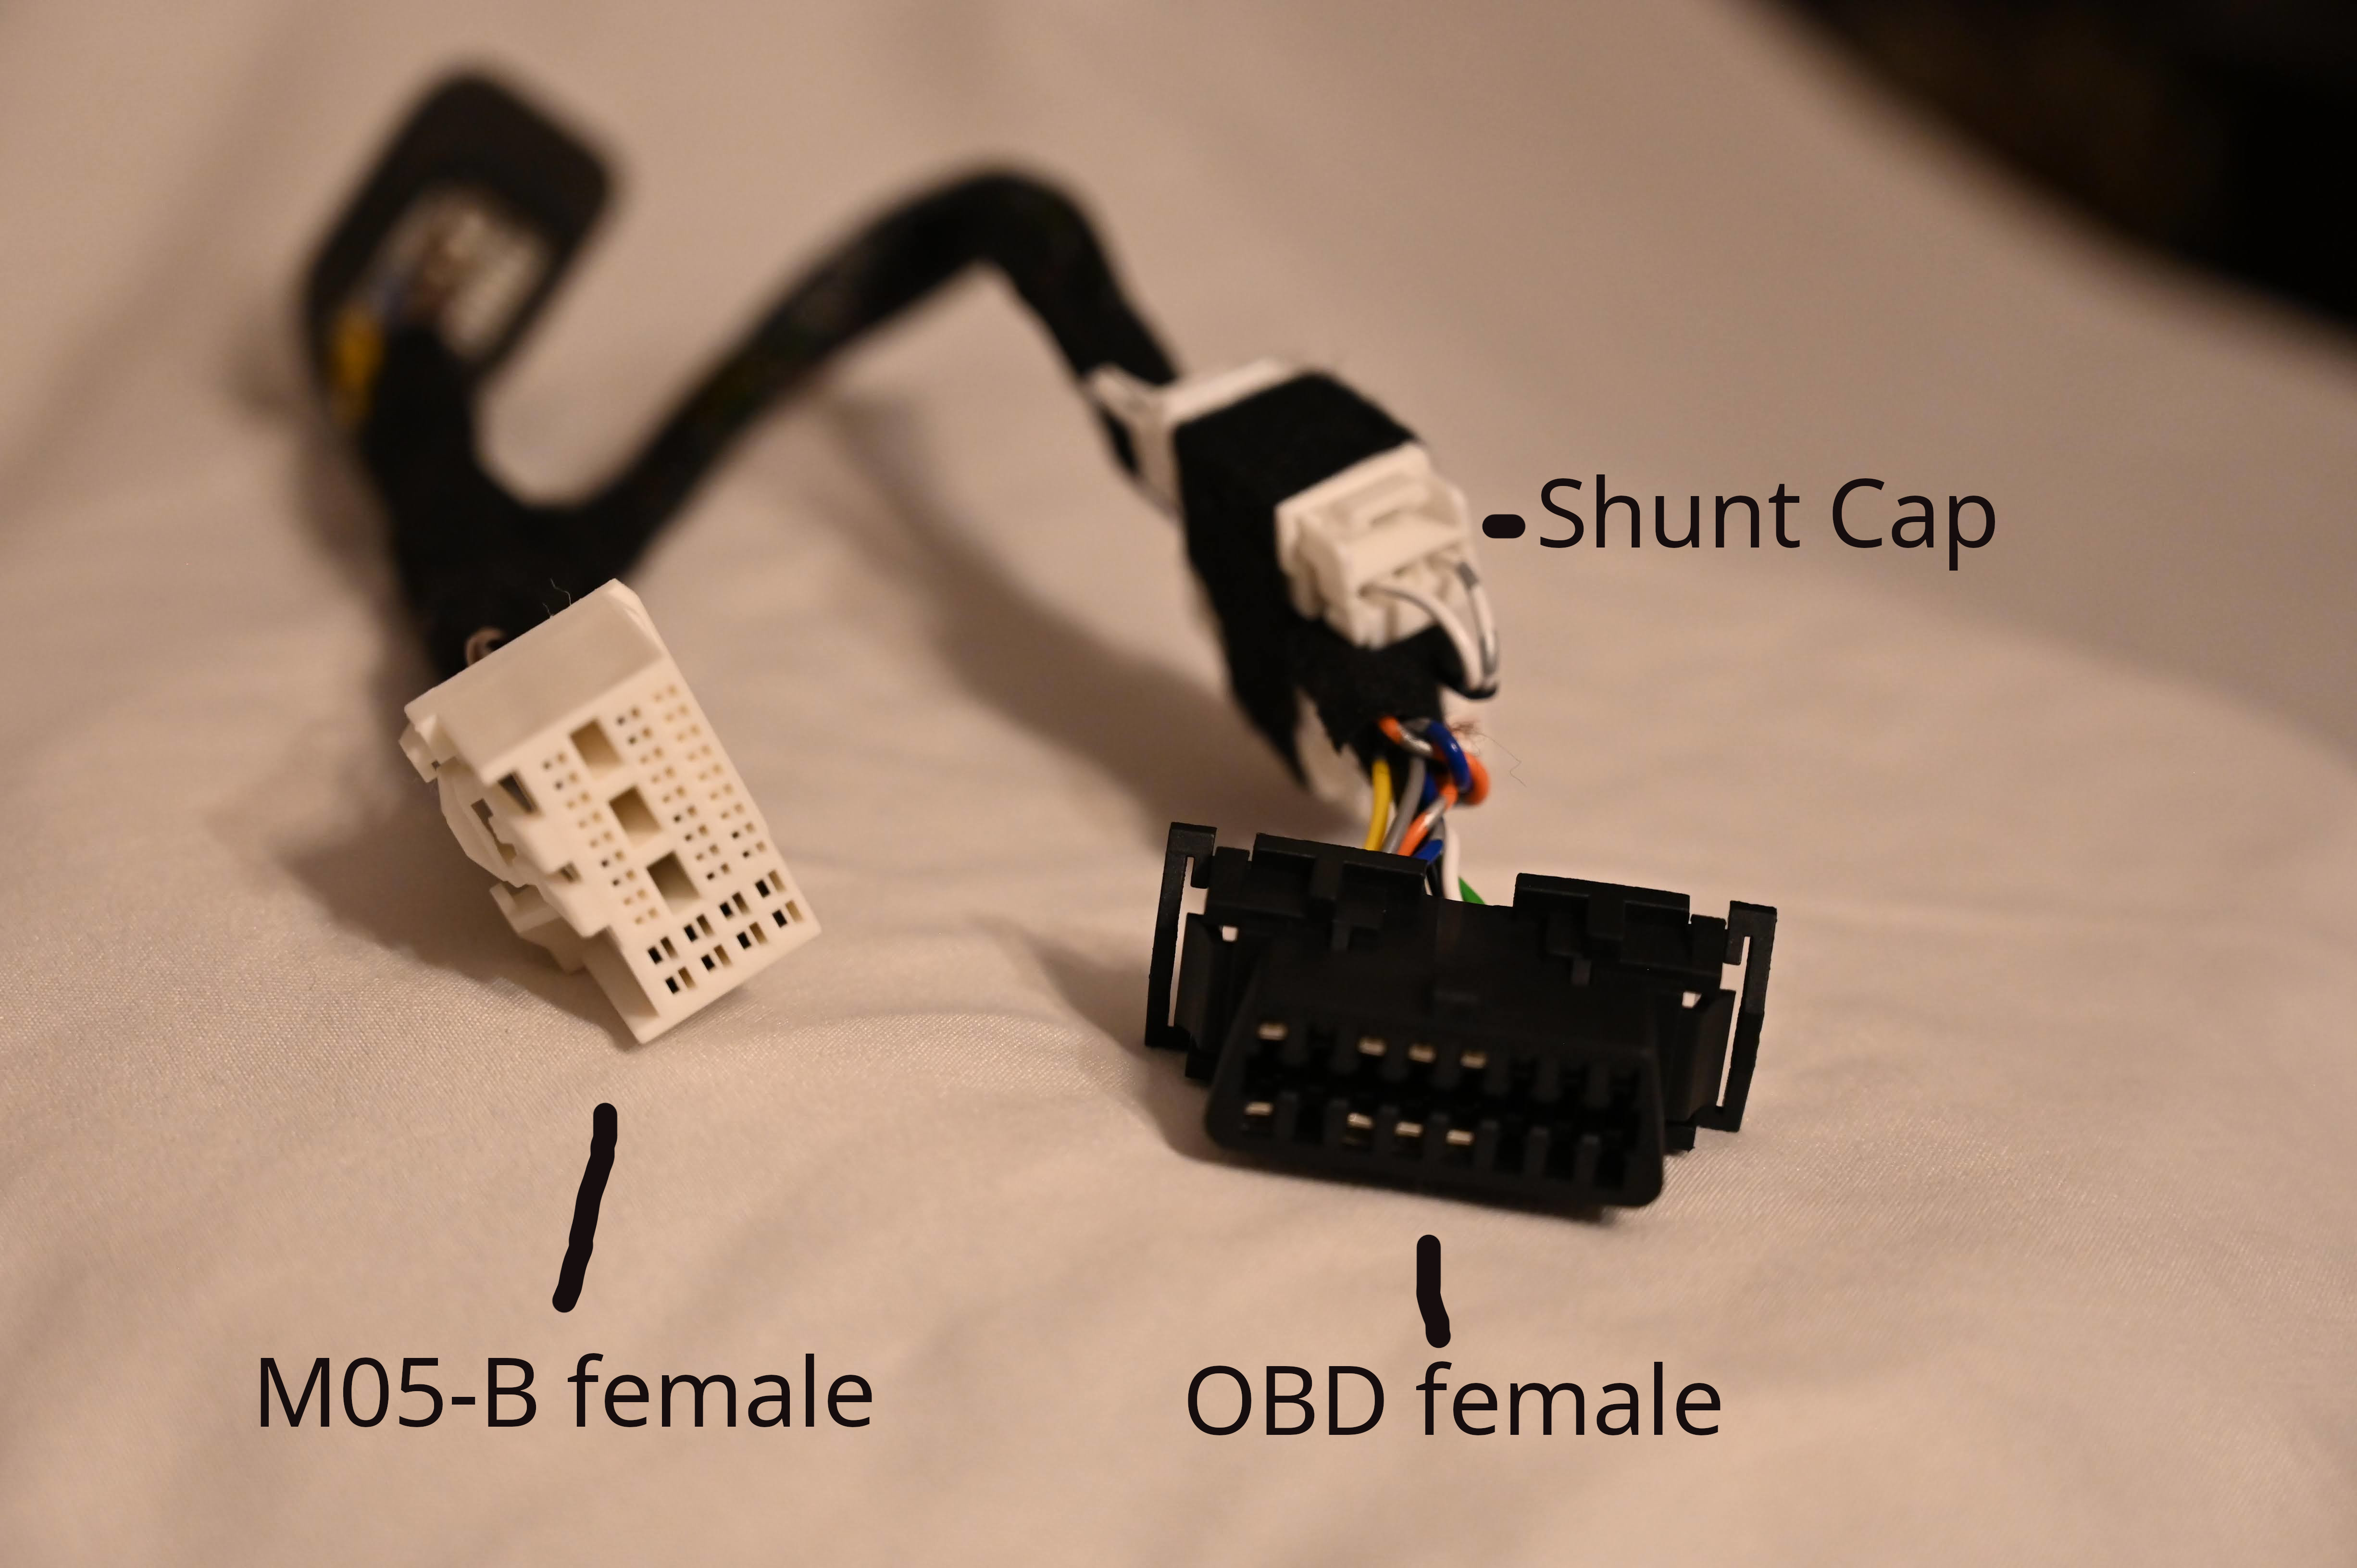
\includegraphics[height=1.5in,angle=0]{../../../harnesses/head_unit_MITM/photos/labeled_connectors_MITM_harness.jpg} } 
  \subfloat[]{\label{subfig:harness:male}
  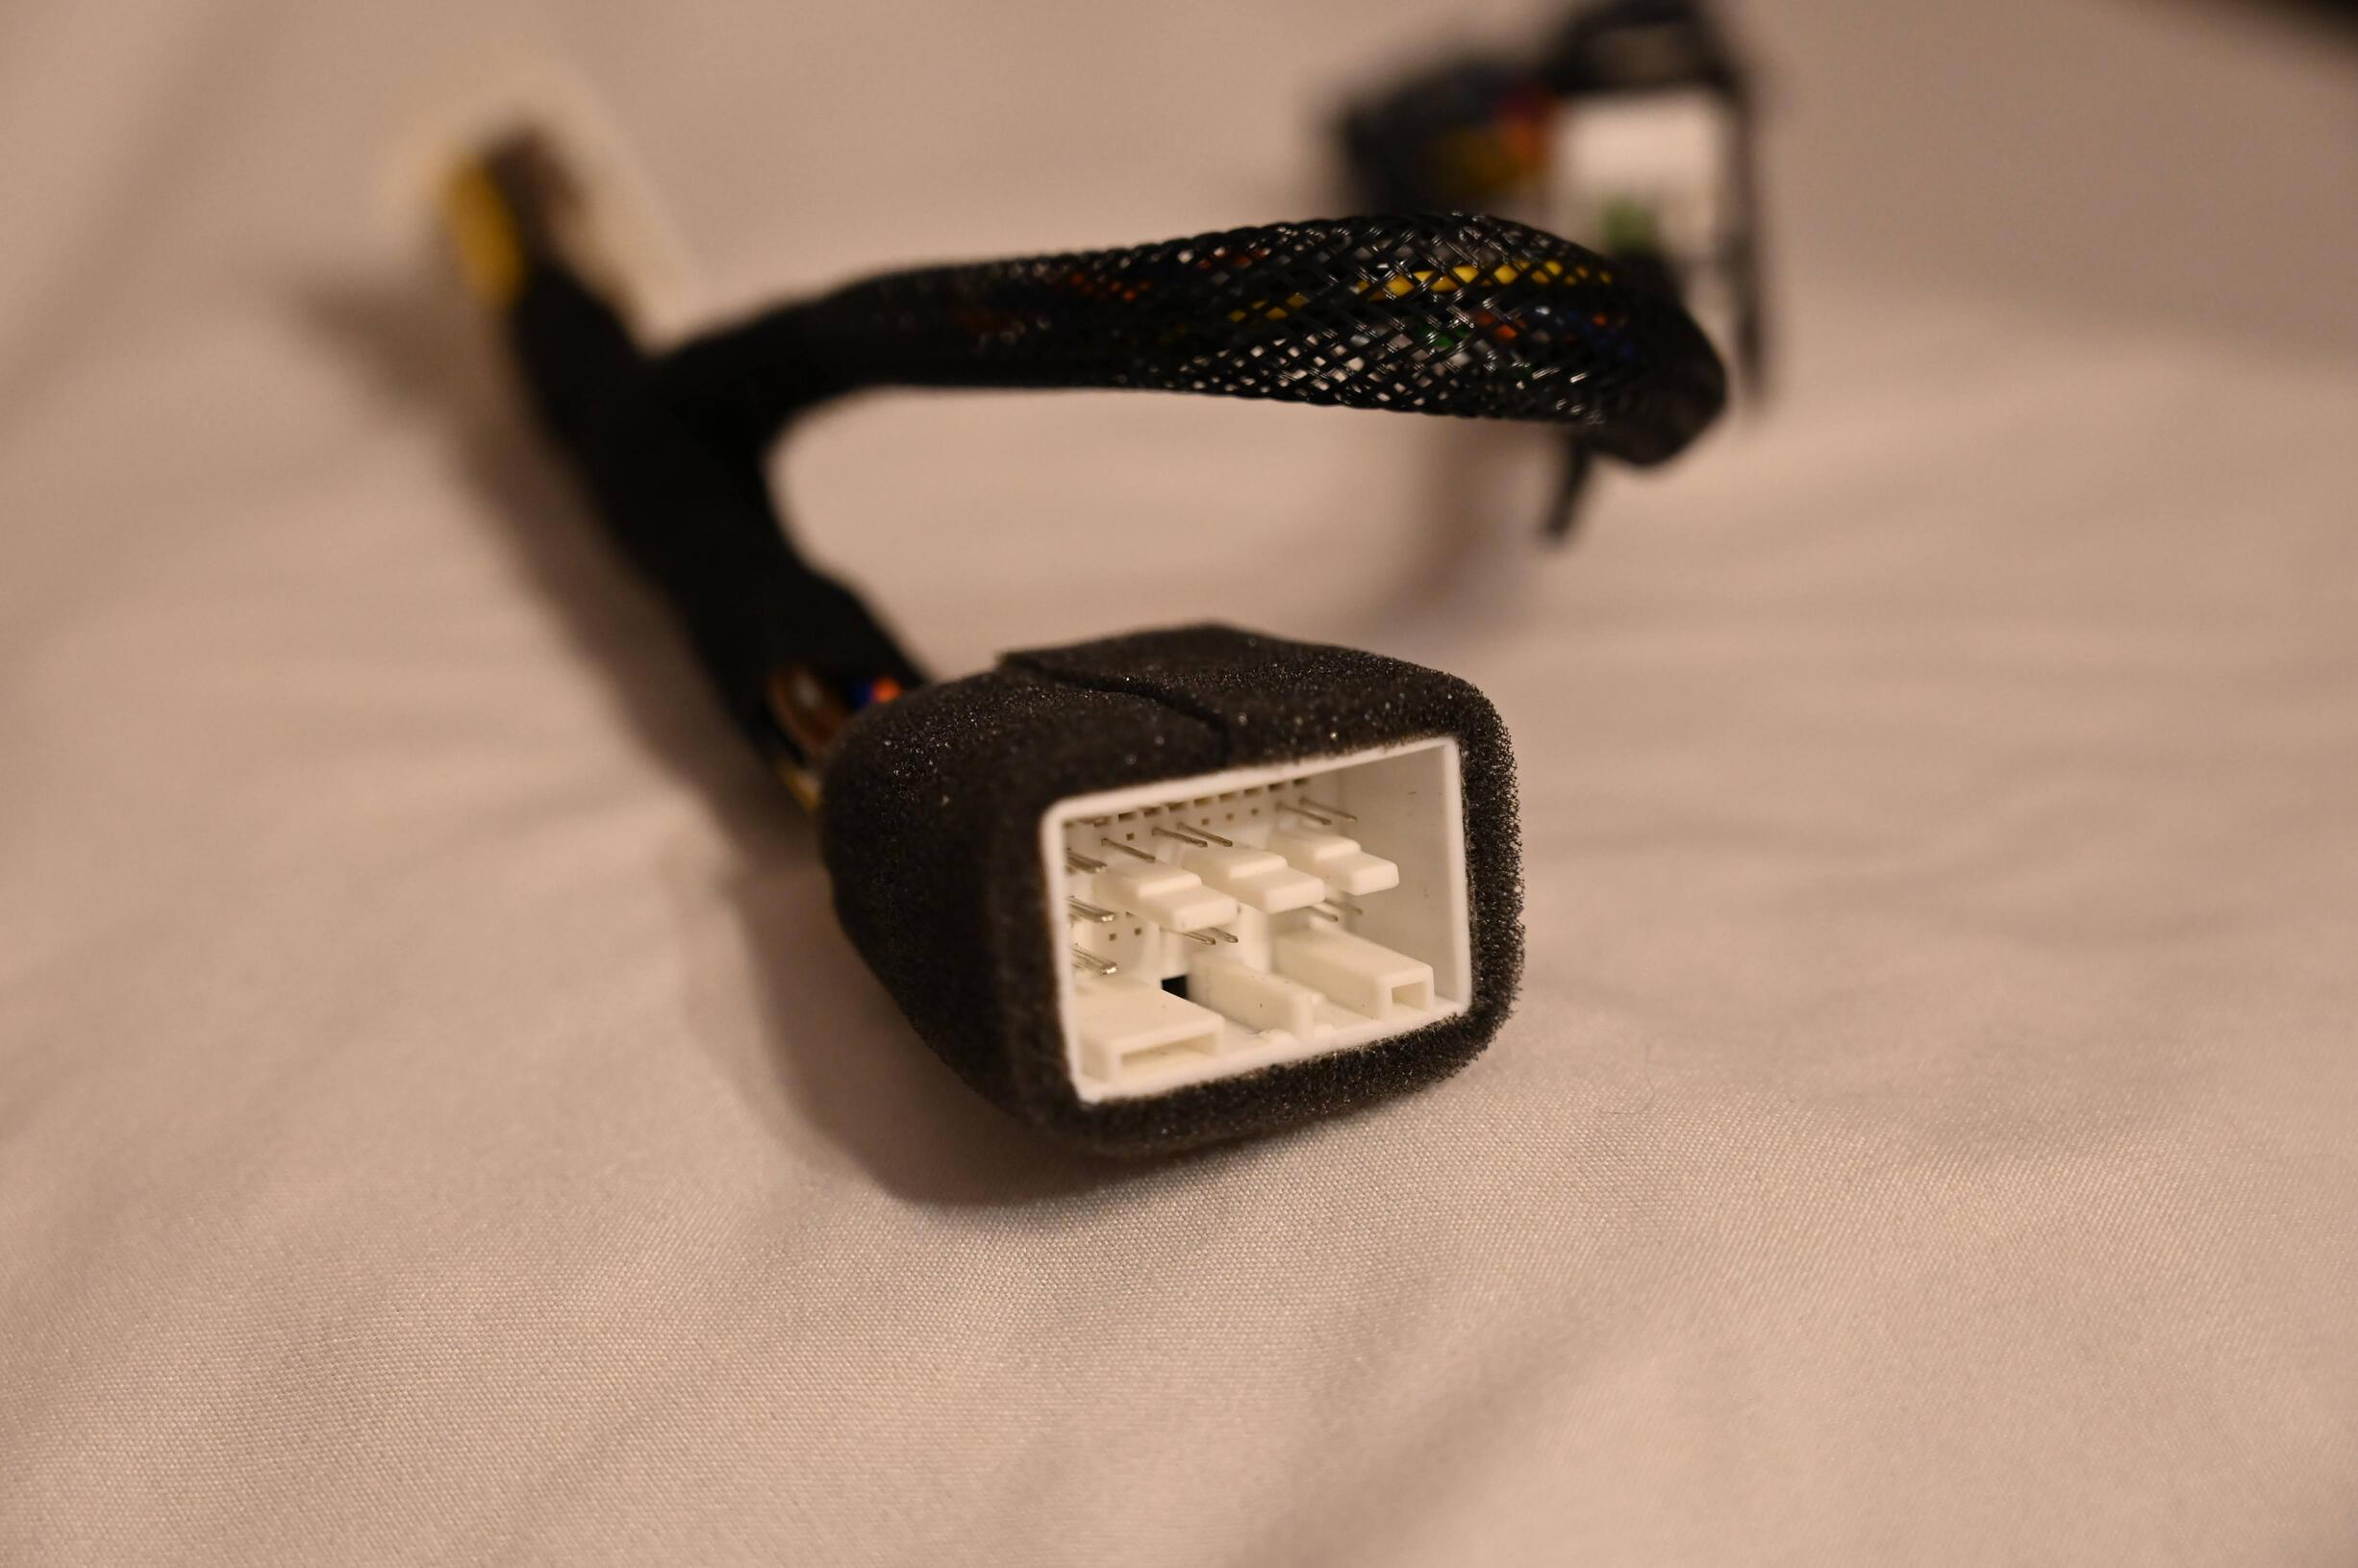
\includegraphics[height=1.5in,angle=0]{photos/male_harness_end.jpg} }  \\
  \subfloat[]{\label{subfig:harness:headunit}
  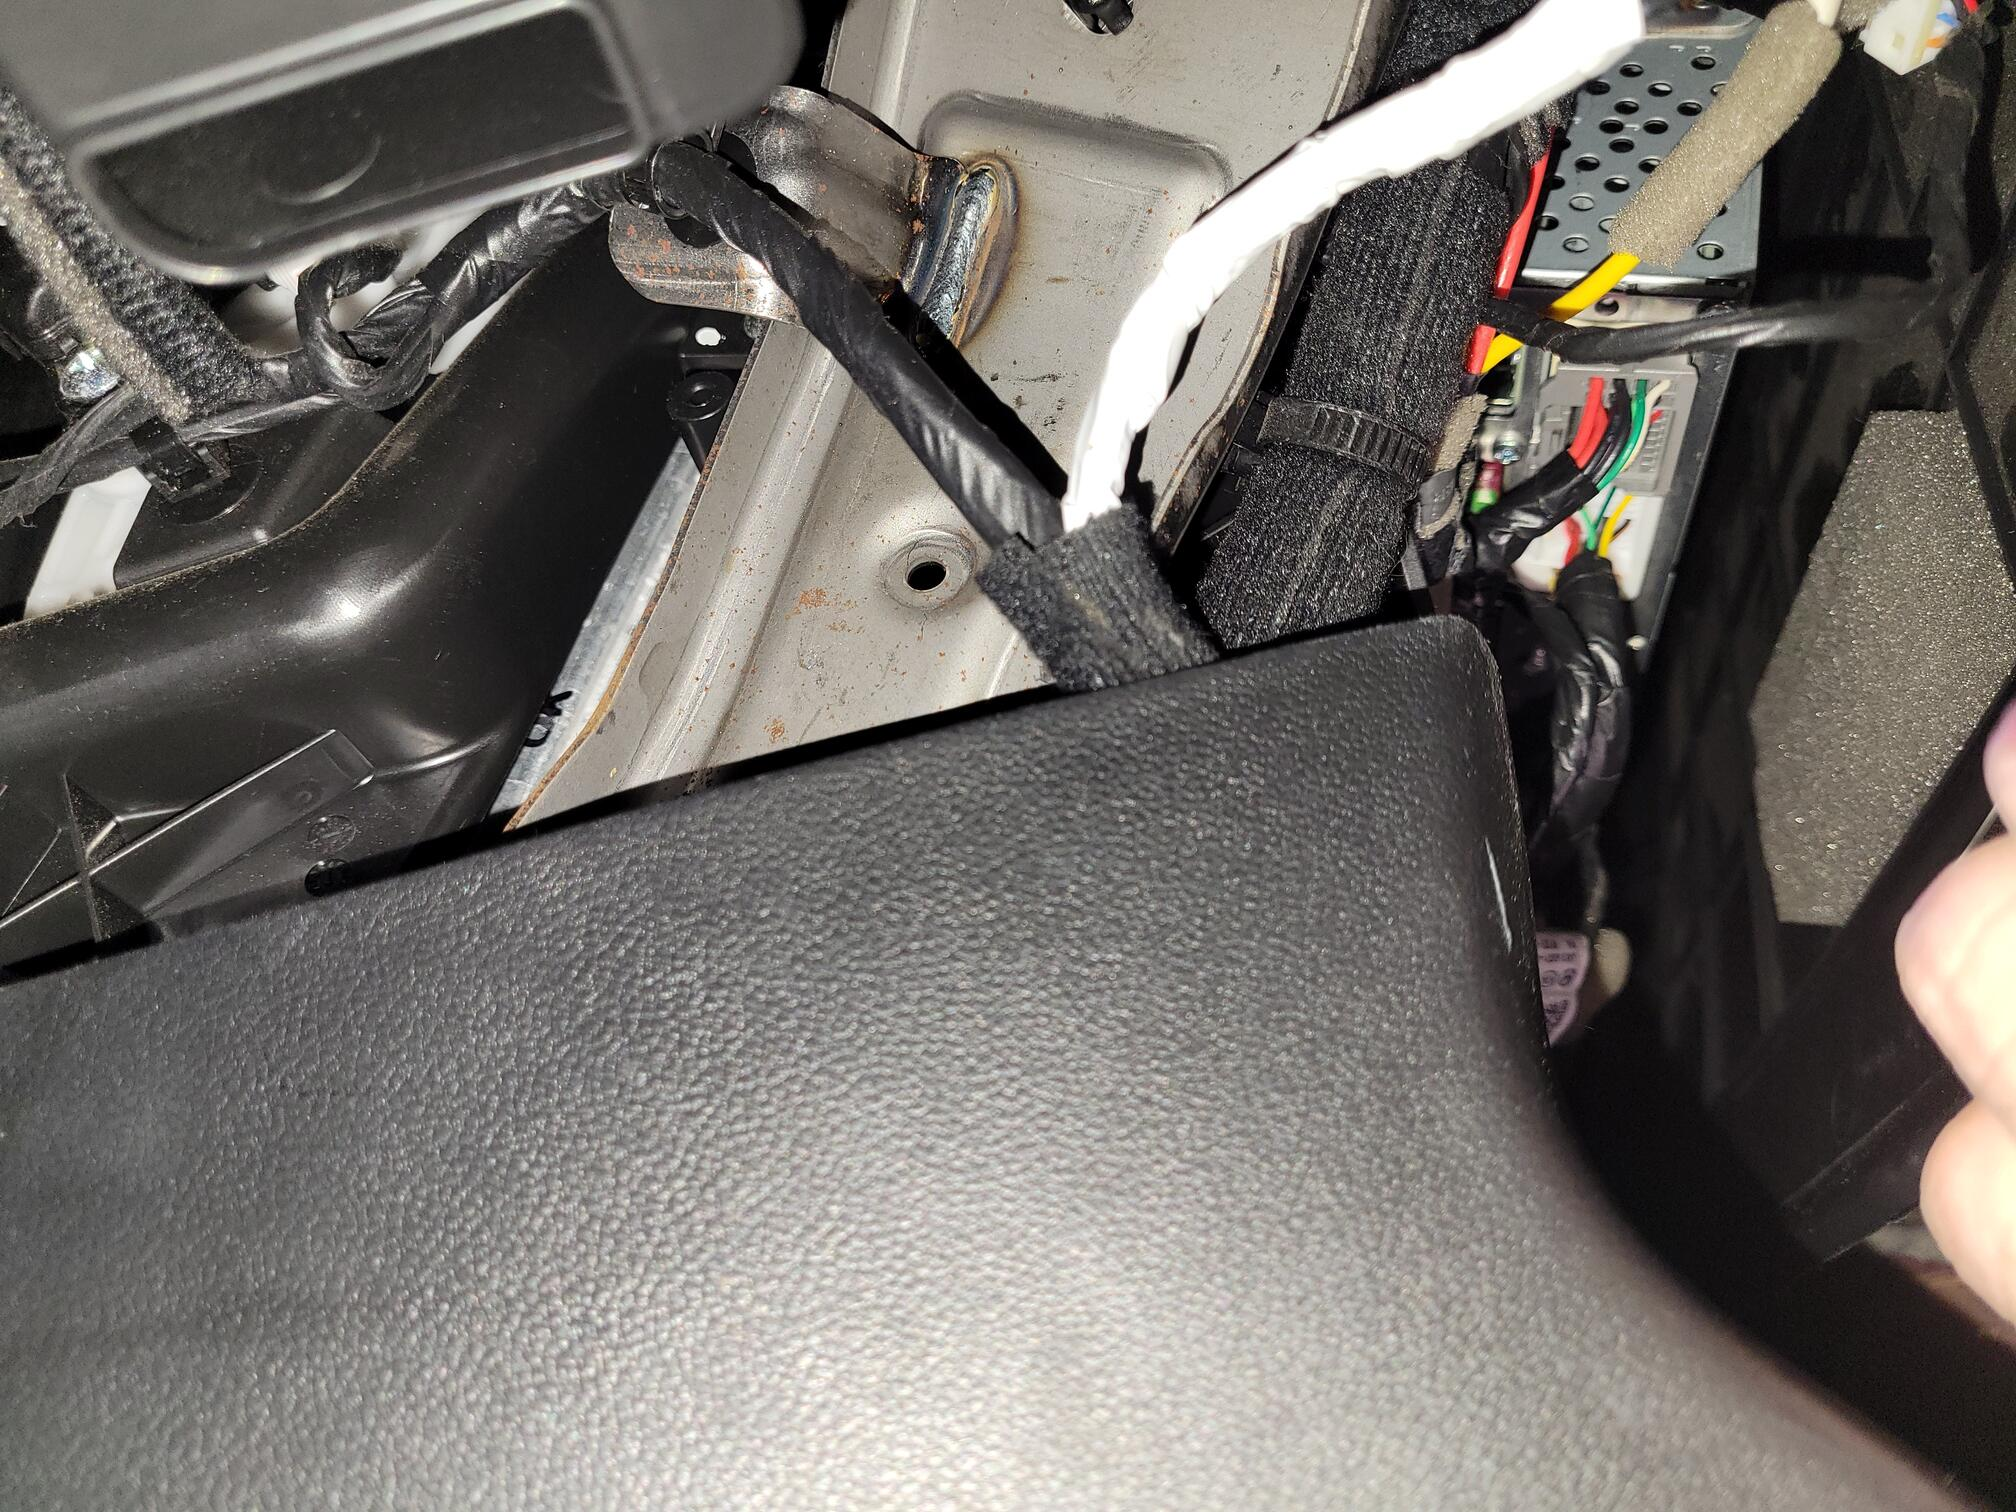
\includegraphics[height=1.5in,angle=0]{photos/head_unit_connectors_in.jpg} } 
  \subfloat[]{\label{subfig:harness:M05Bout}
  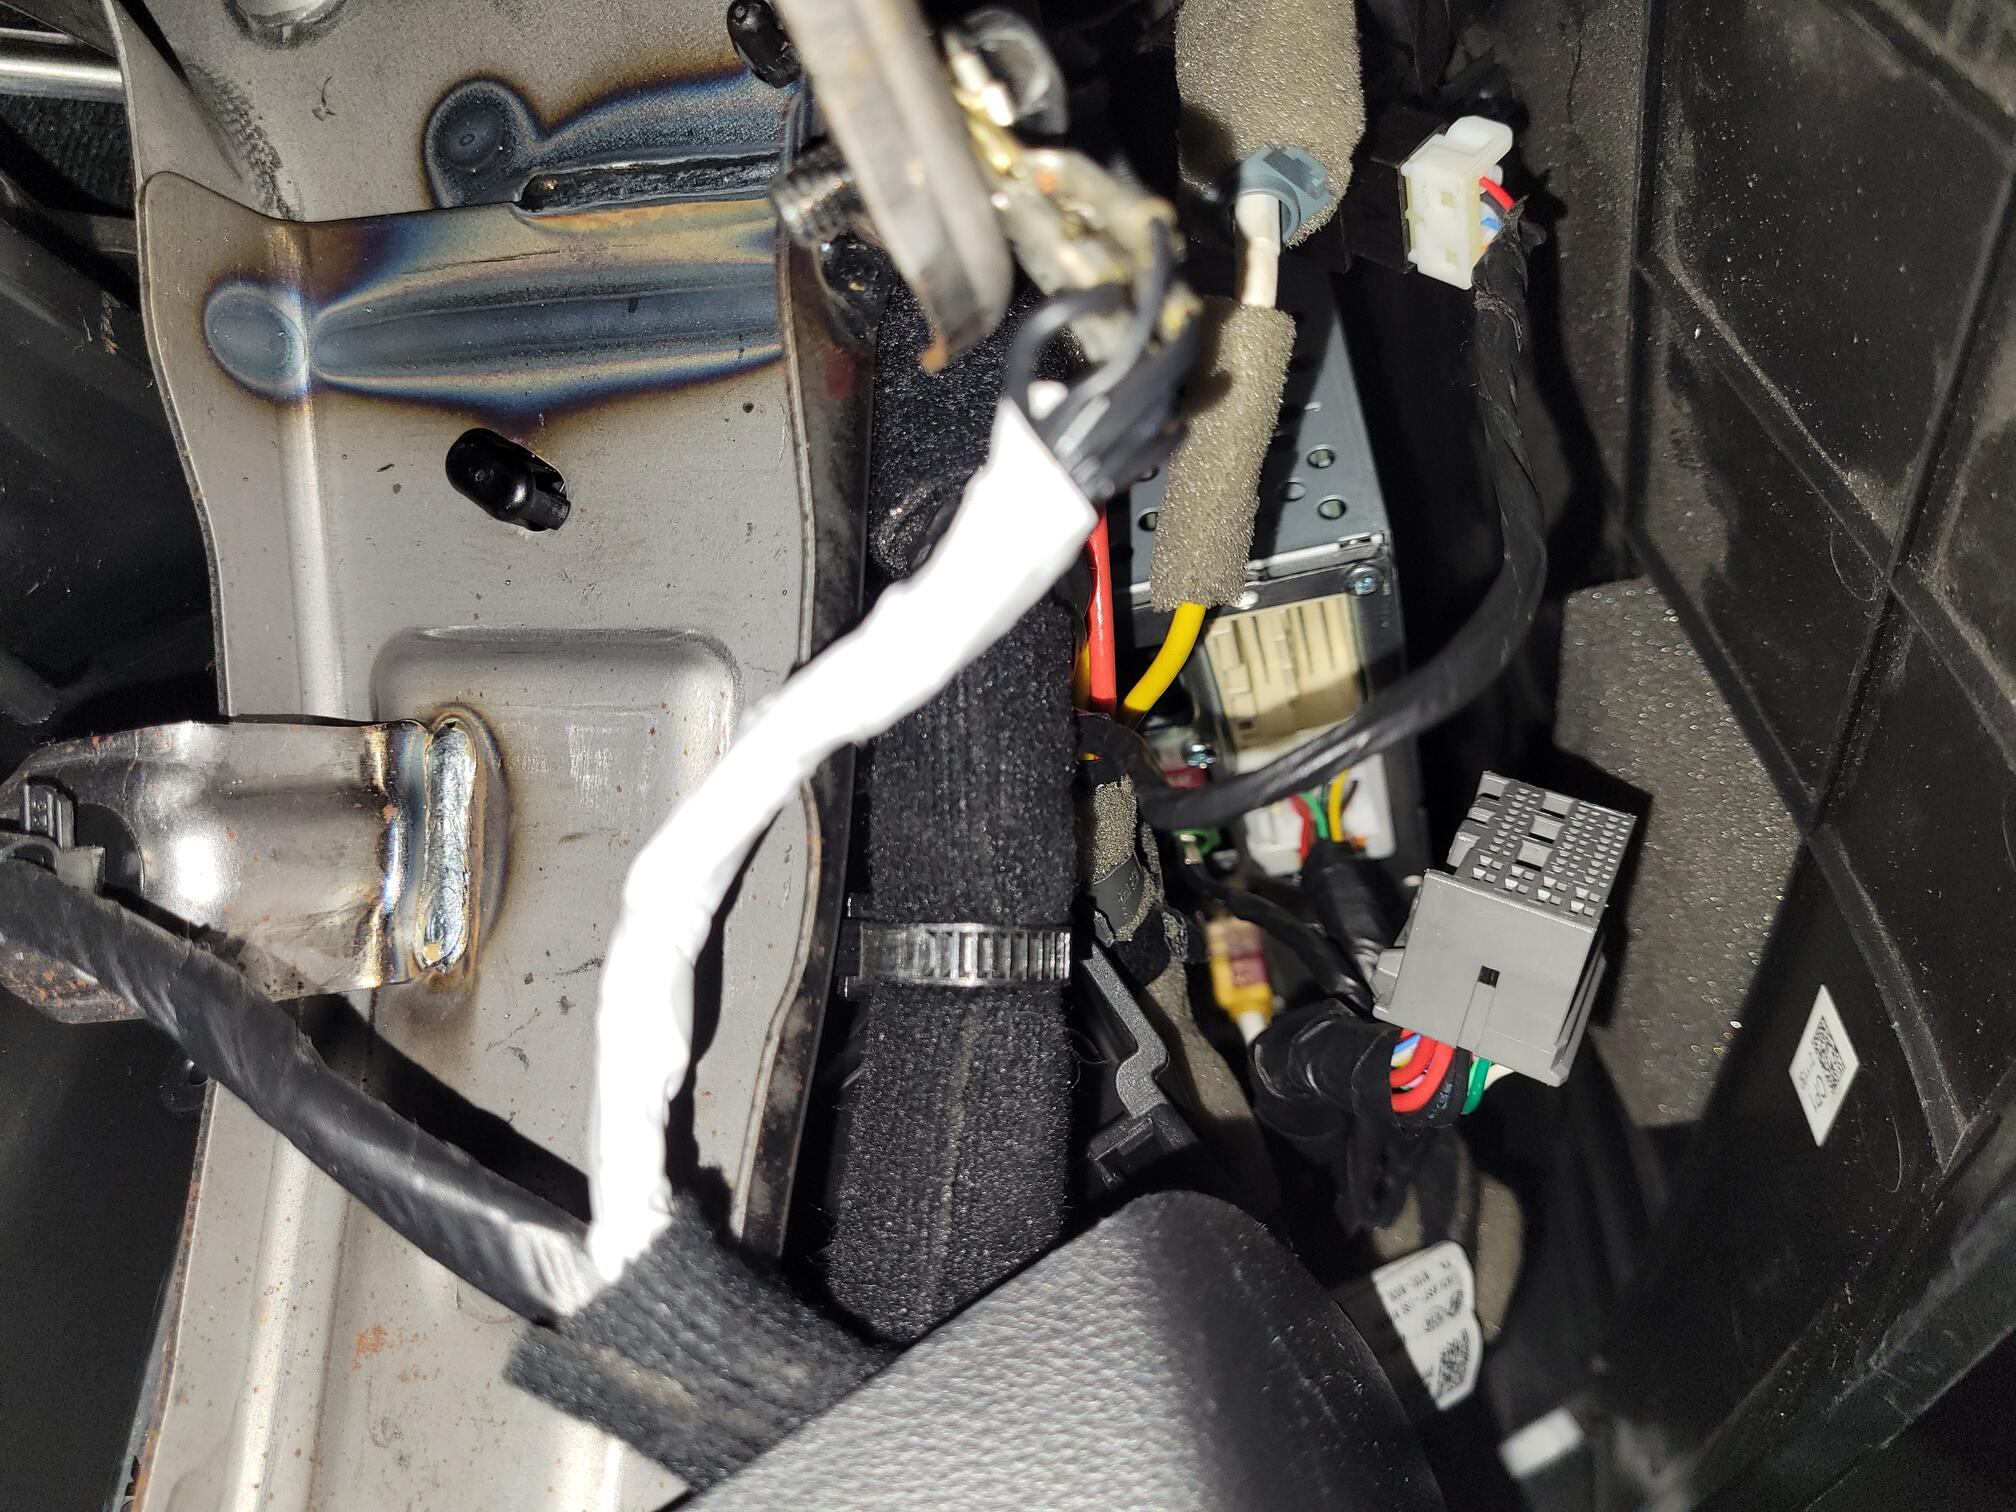
\includegraphics[height=1.5in,angle=0]{photos/M05-B_out.jpg} } 
  \subfloat[]{\label{subfig:harness:harness_in}
  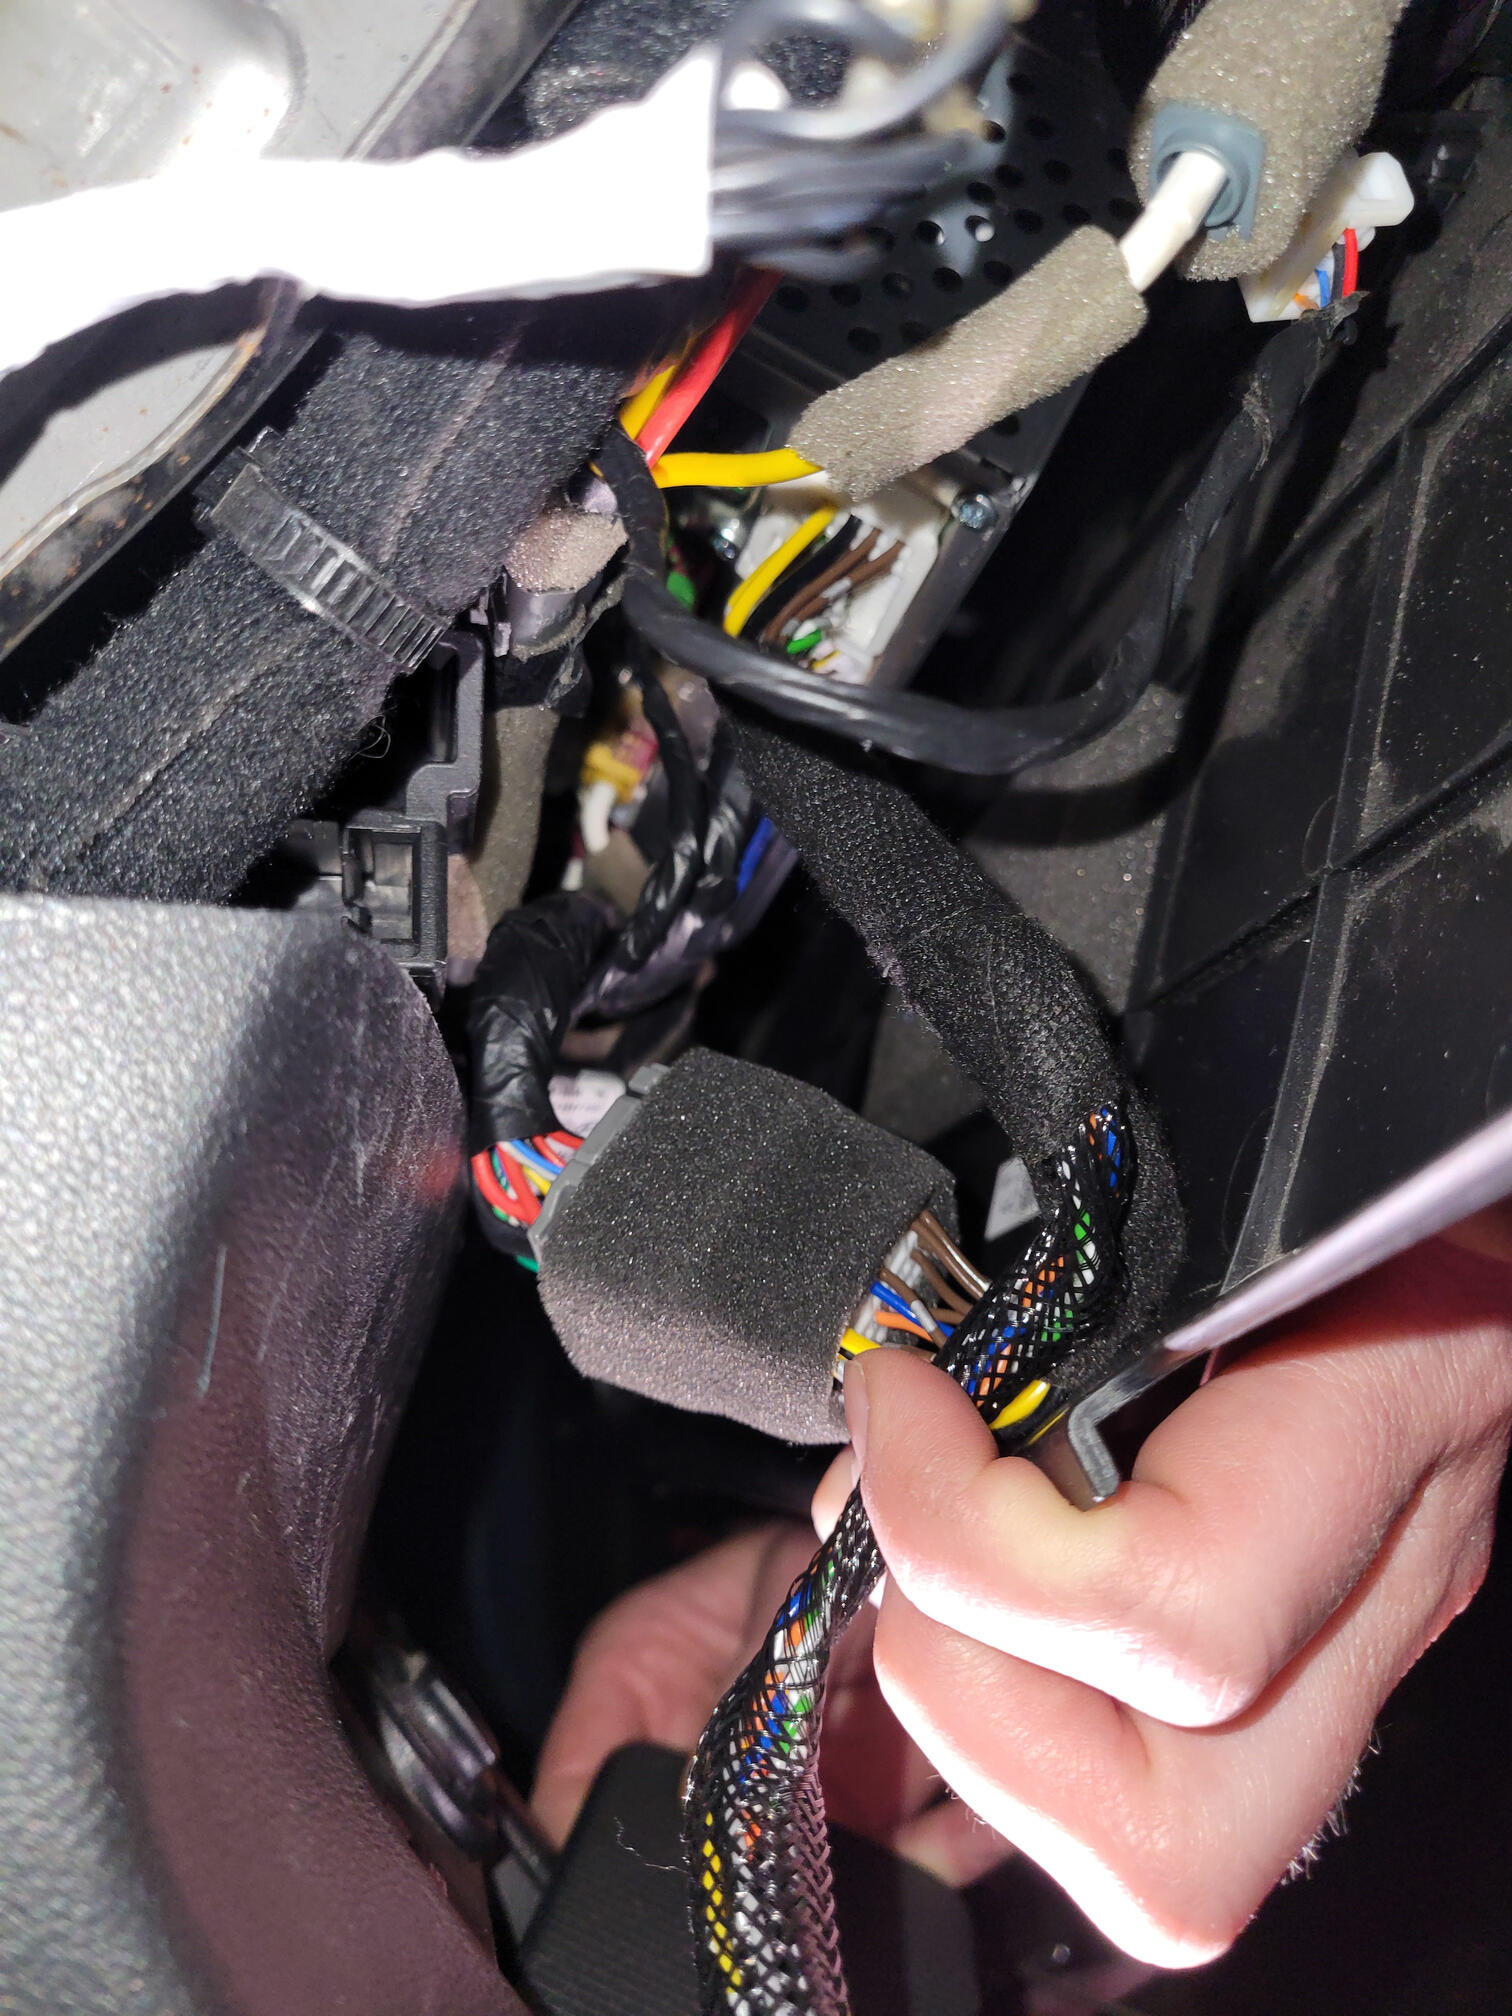
\includegraphics[height=1.5in,angle=0]{photos/harness_in.jpg} }  
   \caption{(a) Labeled photo showing female harness connector. (b) Male harness connector. (c) Head unit with connectors plugged in. (d) Female M05-B connector (grey) removed from head unit. (e) Harness installed in head unit. \label{fig:harness}}
\end{figure}
\section{Step 4: OBD Mount} \label{sect:3}
In this step, we mount the OBD end of the harness securely and plug in the WiCAN. 

Step-by-step instructions:
\begin{enumerate}
  \item Thread harness along the bottom edge of crash pad lower
  \item Plug OBD female into bracket
  \item Use double-sided tape to mount bracket to inside of crash pad lower
  \item Use zip ties to attach harness to other wires and mount points (Figure \ref{subfig:obd:zip_tie})
  \item While holding bracket, plug in WiCAN (Figure \ref{subfig:obd:wican})
\end{enumerate}

\begin{figure}[h]
  \subfloat[]{\label{subfig:obd:zip_tie}
  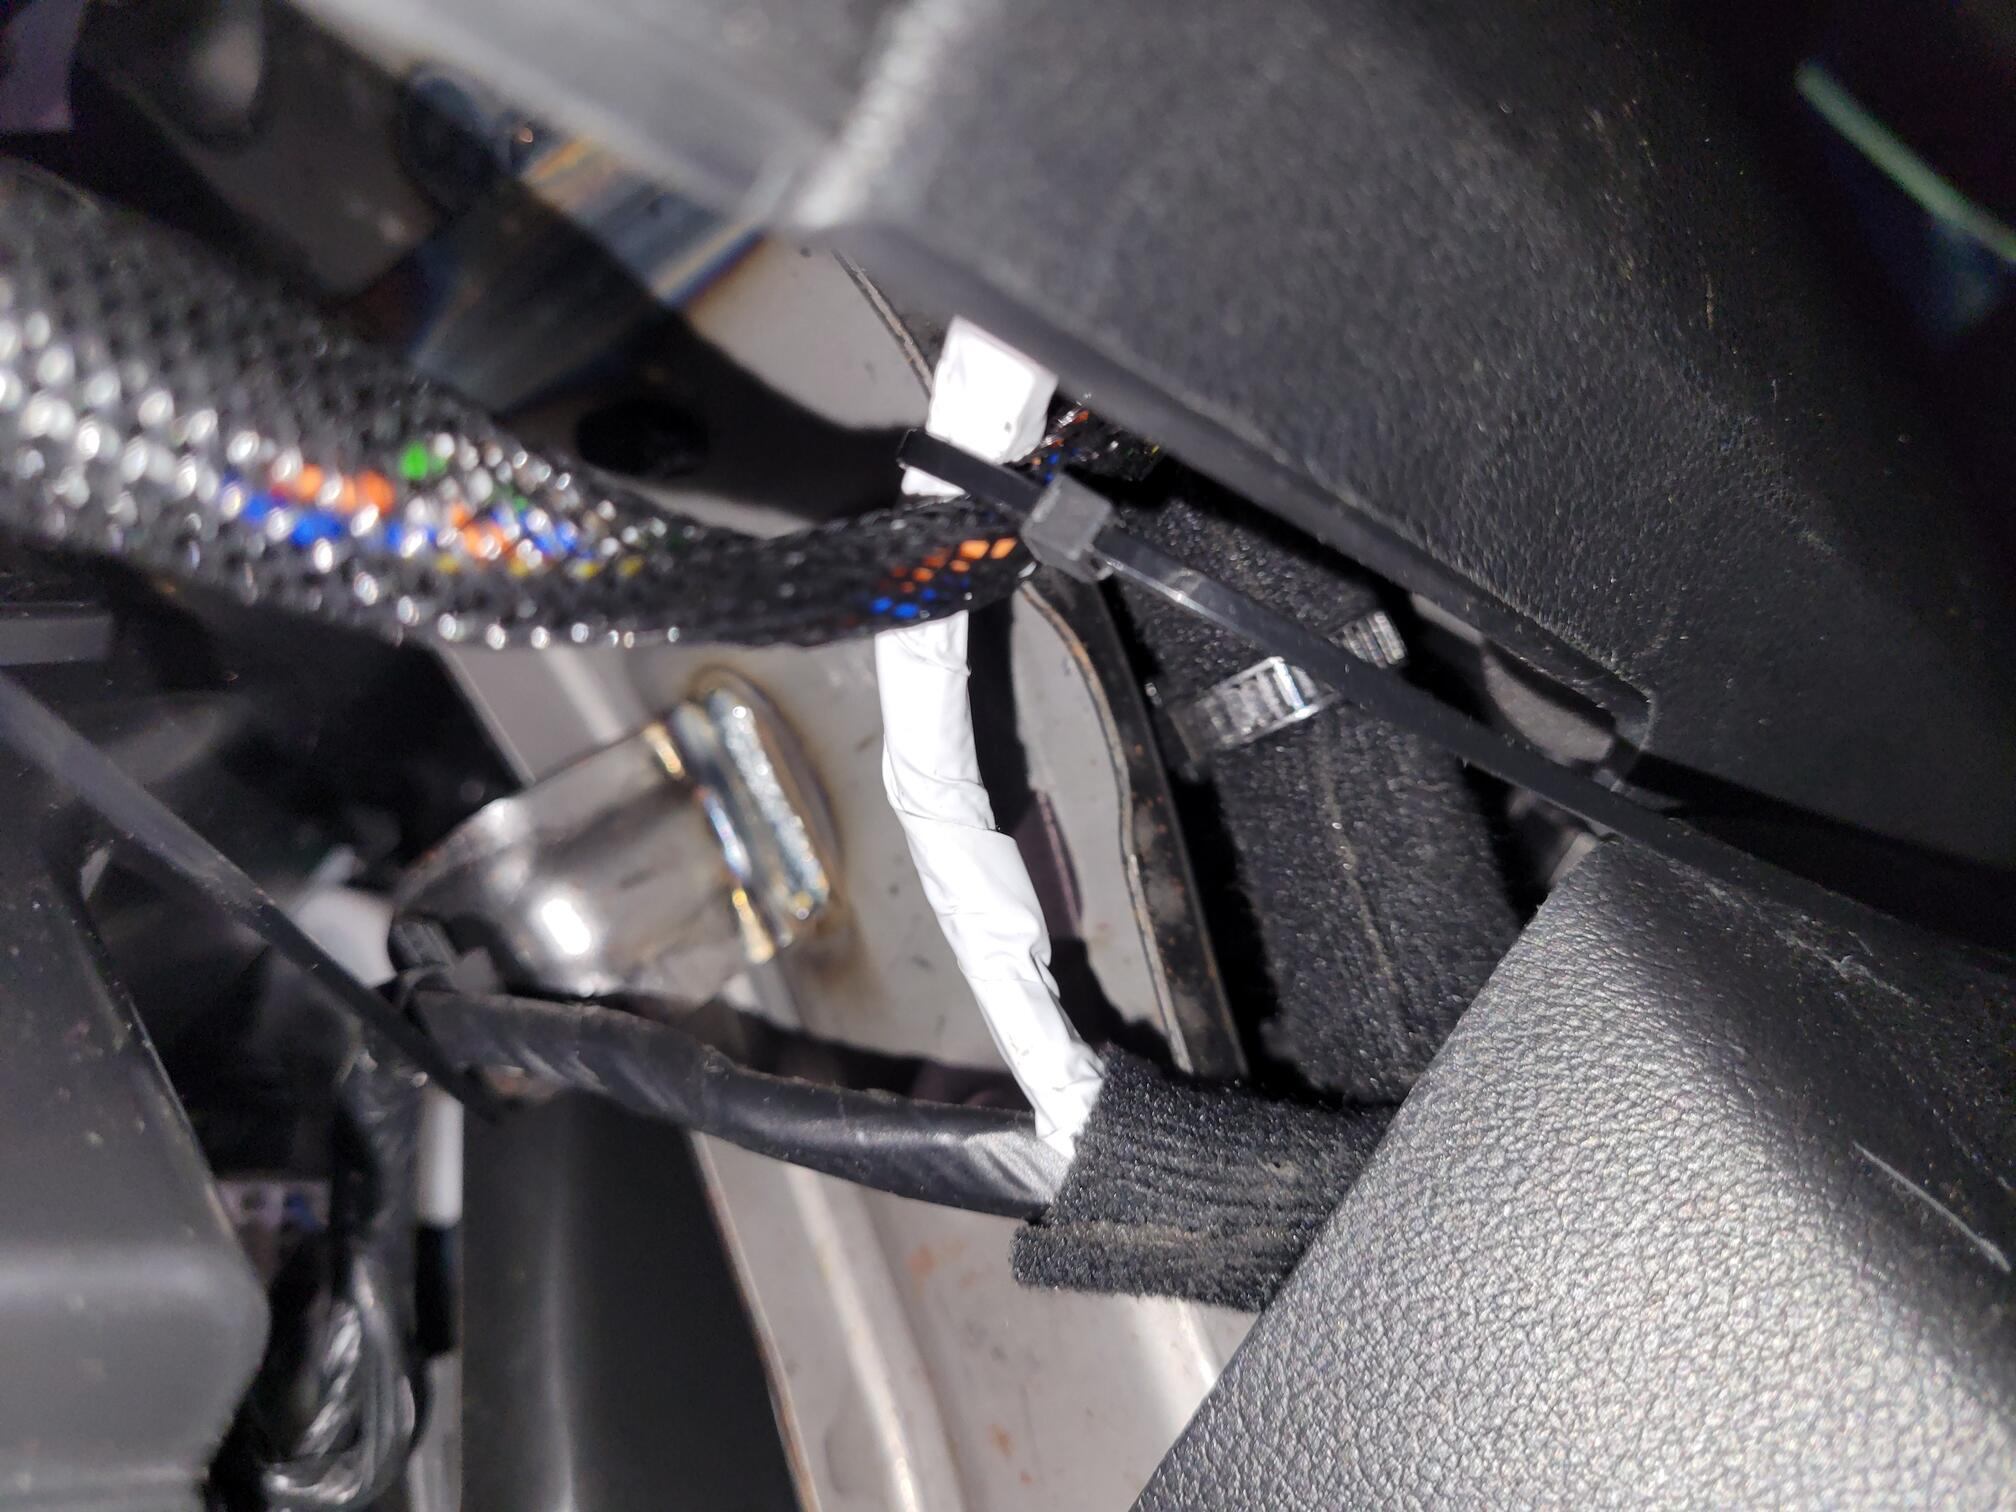
\includegraphics[height=1.5in,angle=0]{photos/zip_tie_1.jpg} } 
  \subfloat[]{\label{subfig:obd:wican}
  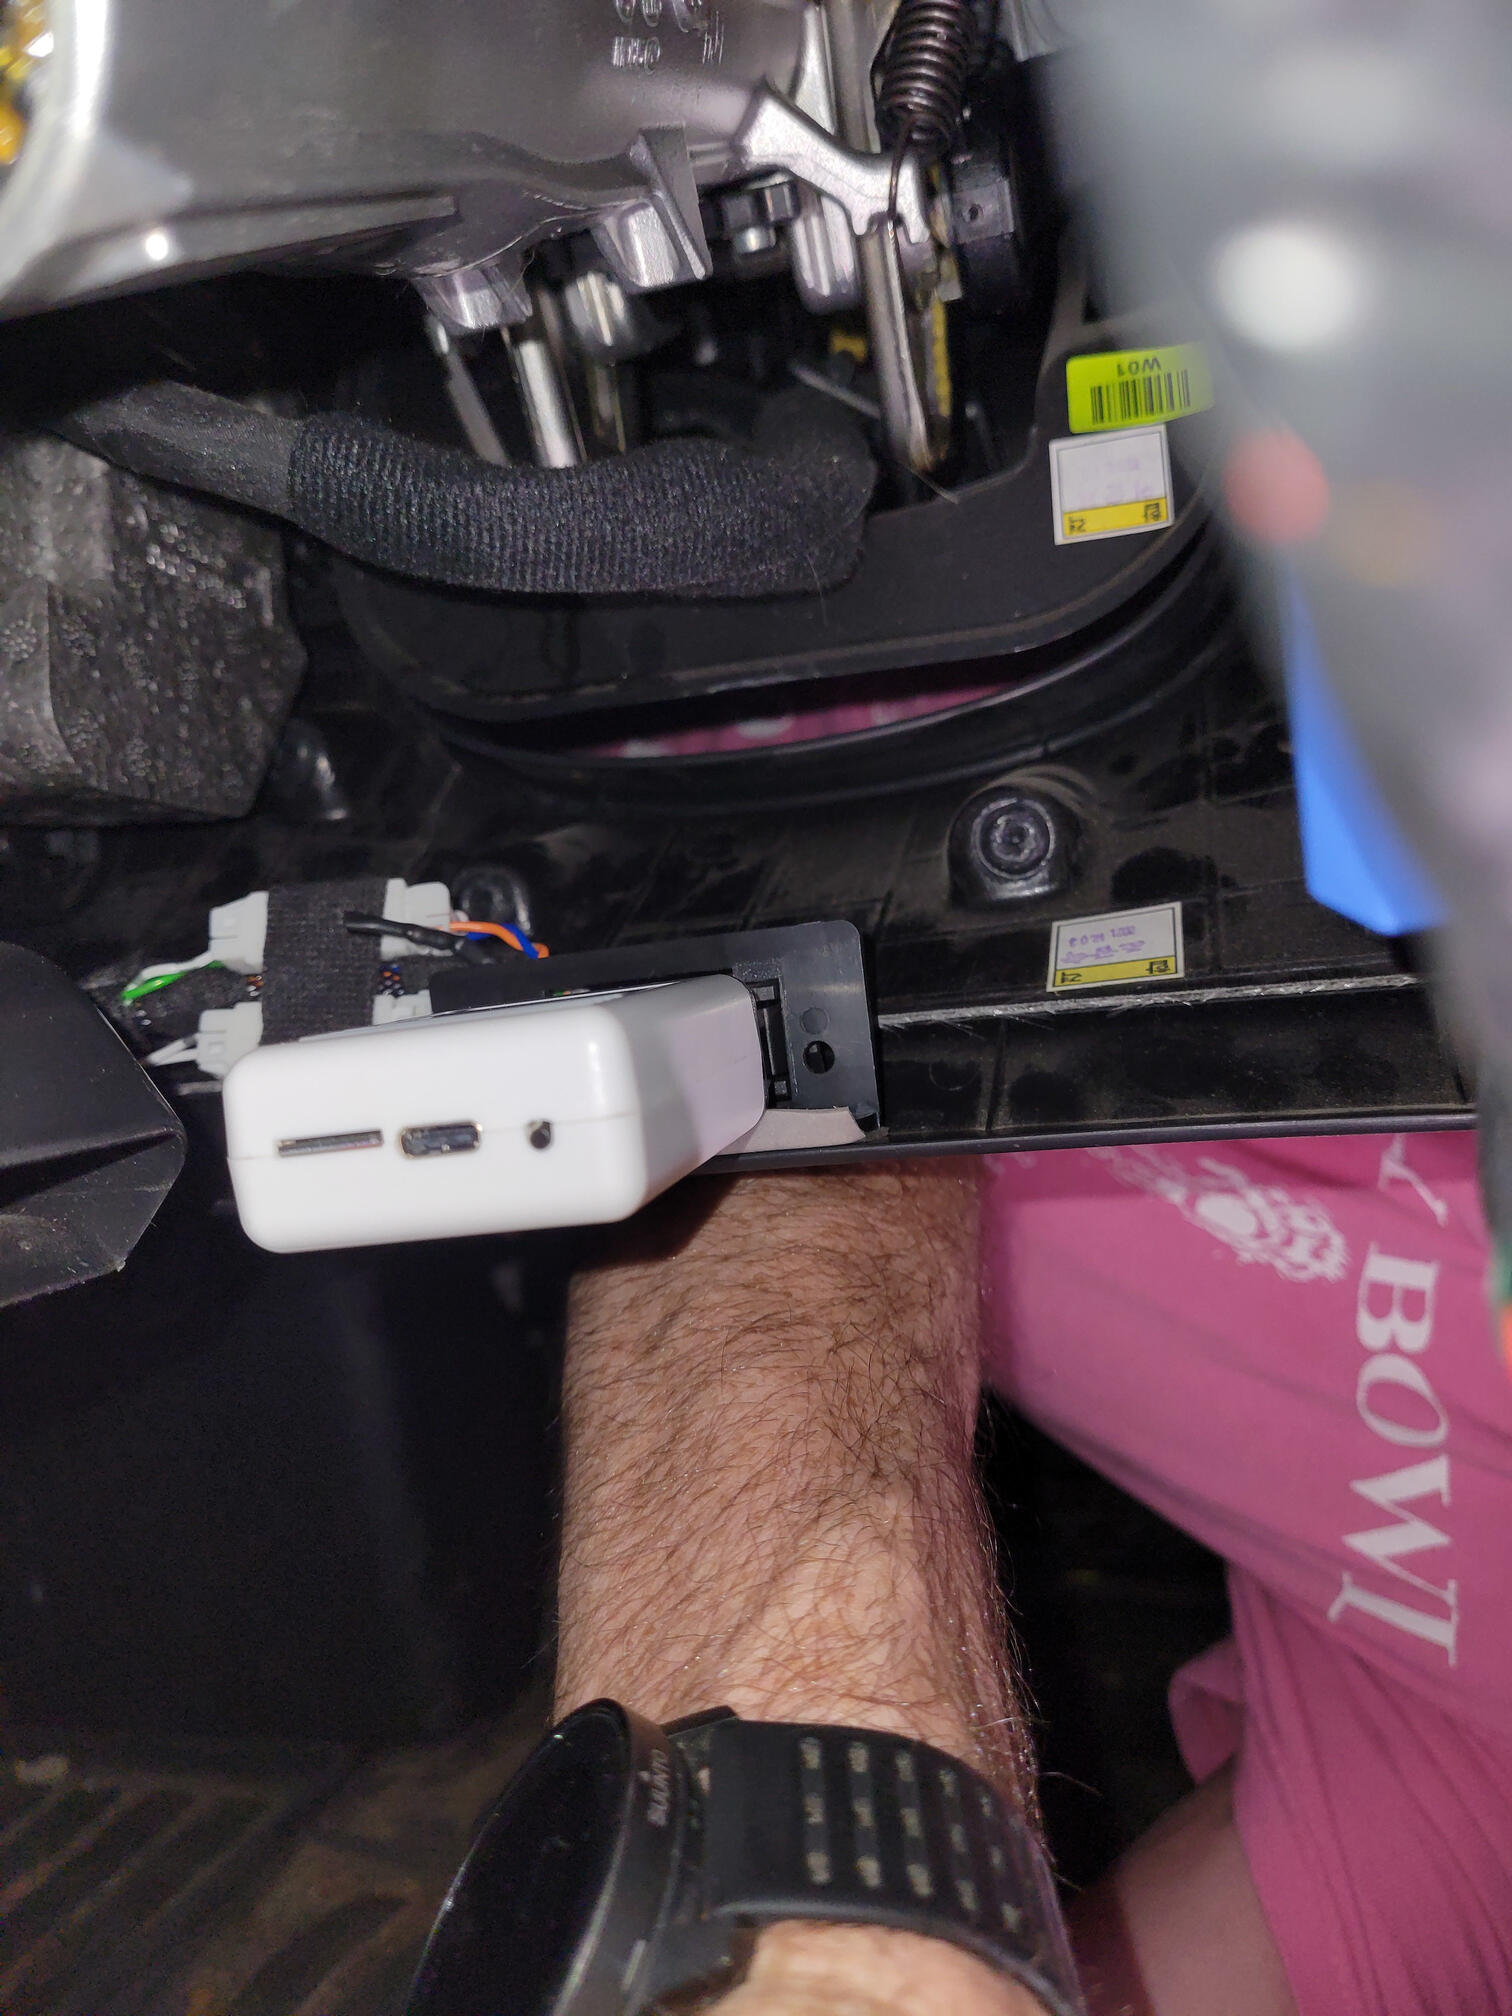
\includegraphics[height=1.5in,angle=0]{photos/wican_inserted.jpg} } 
   \caption{(a) Harness zip-tied to existing wire. (b) WiCAN inserted into OBD. \label{fig:obd}}
\end{figure}

\section{Step 5: Clean up} \label{sect:4}
Reverse the trim removal steps. Make sure trim clips are aligned, and then firmly pop the trim panels back into place. Reconnect 12V battery negative terminal. The WiCAN should immediately show a blue light. \href{https://meatpihq.github.io/wican-fw/config/wifi}{Change your WiCAN password!}. You can connect you your WiCAN directly by finding a WiFi network named 'WiCAN\_xxxxxxx' and going to \href{http://192.168.80.1/}{http://192.168.80.1/} in your browser.
\appendix 
\bibliographystyle{apsrev4-1}
\bibliography{stemh_model}{}
\end{document}
